%
% Sample SBC book chapter
%
% This is a public-domain file.
%
% Charset: ISO8859-1 (latin-1) áéíóúç
%
\documentclass{SBCbookchapter}

\usepackage{cite}
\usepackage{amsmath}
\usepackage{amssymb}
\usepackage{amsthm}
\usepackage{txfonts}
\usepackage[section]{algorithm}
\usepackage{algorithmicx}
\usepackage{algpseudocode}
\usepackage{textcomp}
\usepackage{url}
\usepackage{stfloats}
\usepackage{stackrel}
\usepackage{dsfont}
\usepackage{mathrsfs}
\usepackage{graphicx}
\usepackage{enumerate}
\usepackage{indentfirst}
\usepackage{tikz}
\usepackage{multicol}
%\usepackage{subcaption}
\usepackage{subfigure}

\usepackage[utf8]{inputenc}
\usepackage[T1]{fontenc}
\usepackage[brazilian,english]{babel}

\renewcommand{\refname}{Referências} 
\newcommand{\F}{\mathbb{F}}
\newcommand{\f}{\mathscr{F}}
\newcommand{\G}{\mathbb{G}}
\newcommand{\Samples}{\stackrel{\$}{\gets}}
\newcommand{\Input}{\item[\textsc{Input:}]}
\newcommand{\Output}{\item[\textsc{Output:}]}
\newcommand{\MQ}{\mathcal{MQ}}
\newcommand{\Z}{\mathbb{Z}}
\newcommand{\N}{\mathbb{N}}
\newcommand{\h}{\mathscr{H}}
\newcommand{\tp}{\textrm{\tiny T}}

\newcommand{\ignore}[1]{{}}
\newcommand{\Set}[1]{\{\,#1\,\}}

\floatname{algorithm}{Algoritmo}
\renewcommand{\algorithmicrequire}{\textbf{Entrada:}}
\renewcommand{\algorithmicensure}{\textbf{Saída:}}
\renewcommand{\algorithmicend}{\textbf{fim}}
\renewcommand{\algorithmicif}{\textbf{se}}
\renewcommand{\algorithmicthen}{\textbf{então}}
\renewcommand{\algorithmicelse}{\textbf{senão}}
\renewcommand{\algorithmicfor}{\textbf{para}}
\renewcommand{\algorithmicforall}{\textbf{para todo}}
\renewcommand{\algorithmicdo}{\textbf{faça}}
\renewcommand{\algorithmicwhile}{\textbf{enquanto}}
\renewcommand{\algorithmicloop}{\textbf{laço}}
\renewcommand{\algorithmicrepeat}{\textbf{repita}}
\renewcommand{\algorithmicuntil}{\textbf{até}}
\renewcommand{\algorithmicreturn}{\textbf{retorne}}
\algtext*{EndWhile}% Remove "end while" text
\algtext*{EndIf}% Remove "end if" text
\algtext*{EndFor}% Remove "end if" text

\newcommand{\samples}{\mathop{\stackrel{\ _\$}{\gets}}}

\DeclareMathOperator{\KeyGen}{KeyGen}
\DeclareMathOperator{\Enc}{Enc}
\DeclareMathOperator{\Dec}{Dec}
\DeclareMathOperator{\DualKeyGen}{DualKeyGen}
\DeclareMathOperator{\DualEnc}{DualEnc}
\DeclareMathOperator{\DualDec}{DualDec}

%Notacoes de códigos corretores
\DeclareMathOperator{\dist}{dist}
\DeclareMathOperator{\wt}{wt}
\DeclareMathOperator{\toep}{toep}
\DeclareMathOperator{\vdm}{vdm}
\DeclareMathOperator{\diag}{diag}
\DeclareMathOperator{\GRS}{GRS}
\DeclareMathOperator{\Vol}{Vol}
\DeclareMathOperator{\Det}{det}


% notação BigO
\newcommand{\bigO}[1]{\ensuremath{\mathop{}\mathopen{}\mathcal{O}\mathopen{}\left(#1\right)}}

\newtheorem{theorem}{Teorema}{\bfseries}{\itshape}
\newtheorem{lemma}{Lema}{\bfseries}{\itshape}
\newtheorem{definition}{Definição}{\bfseries}{\itshape}

\setlength{\abovedisplayskip}{0pt}
\setlength{\belowdisplayskip}{0pt}
\setlength{\abovedisplayshortskip}{0pt}
\setlength{\belowdisplayshortskip}{0pt}

\usetikzlibrary{decorations.pathreplacing,calc}
\usetikzlibrary{arrows}
\usetikzlibrary{circuits}

\usetikzlibrary{circuits.logic.US,circuits.logic.IEC}
\usetikzlibrary{automata}
\usetikzlibrary{trees}
\usepackage{tikz-3dplot}

\usetikzlibrary{shapes,arrows,fit}

\tikzstyle{decision} = [diamond, draw, text width=4.5em, text badly centered, node distance=3cm, inner sep=0pt]
\tikzstyle{block} = [rectangle, draw, text width=3em, text centered, rounded corners, minimum height=2em]
\tikzstyle{blockLarge} = [rectangle, draw, text width=6em, text centered, rounded corners, minimum height=2em, sibling distance=5cm]
\tikzstyle{bola} = [circle, draw, text width=3em, text centered, minimum height=2em, sibling distance=5cm]

\tikzstyle{level 1}=[level distance=2.5cm, sibling distance=2.5cm]
\tikzstyle{level 2}=[level distance=2.5cm, sibling distance=1cm]

\tikzstyle{bag} = [text width=4em, text centered]
\tikzstyle{end} = [circle, minimum width=3pt,fill, inner sep=0pt]


\author{Paulo S. L. M. Barreto, Felipe Piazza Biasi, Ricardo Dahab, Julio César López-Hérnandez, Eduardo Morais, Ana D. Salina de Oliveira, Geovandro C. C. F. Pereira, Jefferson E. Ricardini}
\title{Introdução à criptografia pós-quântica}

\setcounter{chapter}{2}

\begin{document}
\begin{otherlanguage}{brazilian}
\pagestyle{empty}

\maketitle

%\tableofcontents

\begin{resumo}
\begin{otherlanguage}{brazilian}
Em 1997, Peter Shor publicou um algoritmo quântico capaz de fatorar inteiros grandes e de calcular logaritmos discretos em corpos finitos em tempo hábil. Tais problemas estão na base da segurança de técnicas convencionais de criptografia assimétrica  (e.g. RSA, ECC). Isso significa que uma informação criptografada nos dias de hoje não necessariamente estará segura em um momento futuro, caso computadores quânticos tornem-se uma realidade. Felizmente, conjectura-se que alguns esquemas criptográficos baseados em outros problemas computacionais resistem ao ataque de Shor com computadores quânticos e ficaram conhecidos como criptossistemas pós-quânticos, como é o caso de criptossistemas baseados em reticulados, em códigos corretores de erro, sistemas multivariados quadráticos e funções de hash. O objetivo deste minicurso é introduzir noções básicas das principais linhas de pesquisa pós-quântica, bem como apresentar os estudos mais recentes de melhorias dos esquemas, relacionadas a tamanhos de chaves, overhead de assinaturas e criptogramas.
\end{otherlanguage}
\end{resumo}


%%%%%%%%%%%%%%%%%%%%%%%%%%%%%%
\section{Introdução}
%%%%%%%%%%%%%%%%%%%%%%%%%%%%%%

Em meados de 1997, Peter Shor introduziu novas preocupações à criptografia ao descobrir um algoritmo quântico capaz de fatorar inteiros grandes e de calcular logaritmos discretos em corpos finitos em tempo hábil \cite{shor}. Isso se deve ao fato de que a segurança de técnicas convencionais de criptografia assimétrica é baseada justamente nesses problemas ou relacionados (e.g. RSA, ECC) \cite{rivest-shamir-adleman,miller}. Desse modo, a segurança efetiva de tais técnicas fica condicionada à construção de um computador quântico de grande porte. Isso significa que uma informação criptografada nos dias de hoje não necessariamente estará segura em um momento futuro por conta da dependência mencionada. 

Outra ameaça ainda mais efetiva são as recentes descobertas de algoritmos clássicos, executados em computadores tradicionais, que são capazes de resolver certos logaritmos discretos usados em criptografia assimétrica \cite{barbulescu}.

Felizmente, conjectura-se que alguns esquemas criptográficos baseados em outros problemas computacionais resistem ao ataque de Shor com computadores quânticos e ficaram conhecidos como criptossistemas pós-quânticos; este é o caso de criptossistemas baseados em reticulados \cite{Goldreich-Goldwasser-Halevi}, códigos corretores de erro \cite{McEliece,Niederreiter}, sistemas multivariados quadráticos ($\MQ$) \cite{ding-schmidt,kipnis-patarin-goubin} e funções de hash~\footnote{O termo ``resumo" (criptográfico), em vez de ``hash", tem sido usado sem grande aceitação. Por isso, optamos por ``funções de hash" ou simplesmente ``hash". Dependendo do contexto, hash pode significar também o valor da função de hash num dado argumento. Como plural, usamos ``hashes''.}~\cite{ding-schmidt,dods-smart-stam}, além das construções de criptografia simétrica em geral. 

Por outro lado, o principal desafio em criptografia assimétrica pós-quântica é a redução no tamanho das chaves públicas e privadas, além do \emph{overhead} de espaço considerável por mensagem a ser assinada ou encriptada. Nesse sentido, há um esforço em pesquisa~\cite{bernstein-buchmann-dahmen} para tornar essas técnicas mais eficientes e competitivas com técnicas convencionais, em relação às métricas mencionadas. Vale ressaltar que, em se tratando do tempo de processamento, tamanho de código fonte e ocupação de memória RAM, muitos esquemas pós-quânticos já são competitivos e muitas vezes superam esquemas convencionais.

Tendo em vista o novo paradigma de Internet das coisas, onde objetos quaisquer são dotados de capacidade computacional própria e capazes de conectar-se à internet, podendo atualizar-se de forma autônoma e estabelecer redes interconectadas. Um efeito colateral dessa interconectividade é uma possível vulnerabilidade destes sistemas embarcados. Ataques que têm sido primariamente voltados a PCs podem, ser lançados contra carros, aparelhos celulares, \emph{e-tickets}, RFIDs. 

Neste cenário, os dispositivos são caracterizados por apresentarem tipicamente escassez no fornecimento de energia (via bateria) e capacidade limitada de processamento, armazenamento e muitas vezes canais de comunicação com baixa largura de banda (e.g. SMS).

Uma vez que sistemas embarcados são normalmente implantados em larga escala, os custos tornam-se uma das principais preocupações dos projetistas. Logo, soluções de segurança para embarcados devem apresentar baixo custo, que pode ser atingido com o projeto de soluções que minimizem \emph{overhead} de transmissão, processamento e ocupação de memória. Nesse sentido as técnicas de criptografia simétrica em geral já atendem as métricas necessárias, sendo a criptografia assimétrica o gargalo na maior parte dos casos.

Primitivas criptograficas assimétricas para encriptação e assinatura digital são essenciais dentro de um 
arcabouço de segurança moderno. Mas as técnicas convencionais não são suficientemente eficientes em certos aspectos, o que dificulta sua utilização em plataformas embarcadas de baixo poder computacional. Nesse contexto a ausência de operações custosas (operações com inteiros grandes, principalmente exponenciações modulares) das técnicas pós-quânticas as torna mais atraentes em cenários de recursos computacionais escassos, como os descritos anteriormente.

O objetivo do minicurso é introduzir noções básicas das principais linhas de \\pesquisa pós-quântica (códigos corretores de erros, sistemas $\MQ$, reticulados e \emph{hash}), bem como apresentar os estudos mais recentes visando a melhorias dos esquemas relacionadas a tamanhos de chaves, overhead de assinaturas e criptogramas.


%%%%%%%%%%%%%%%%%%%%%%%%%%%%%%%%%%%%%%%%%%%%%%%%%%%%%%%%%%%%%%%%%%%%%%%
\section{Esquemas de assinatura digital baseados em funções de hash}
%%%%%%%%%%%%%%%%%%%%%%%%%%%%%%%%%%%%%%%%%%%%%%%%%%%%%%%%%%%%%%%%%%%%%%%
Esquemas de assinatura digital baseados em funções de hash popularizaram-se após o trabalho de Ralph Merkle~\cite{merkle:79} em 1979. 
O esquema proposto por Merkle~\textit{(MSS)} é inspirado no esquema de assinatura \textit{one-time} de Lamport e Diffie~\cite{lamport:79}.
A segurança de tais esquemas é baseada na resistência à colisão e na resistência à inversão da função de hash utilizada. O esquema \textit{(MSS)} é considerado prático e resistente aos computadores clássicos e quânticos, pois não se conhece, na literatura, uma maneira de aplicar o algoritmo de Shor neste esquema. A desvantagem dos esquemas de assinatura digital \textit{one-time} é que uma dada chave privada pode ser utilizada para gerar apenas uma assinatura, embora essa assinatura possa ser verificada um número arbitrário de vezes. 

% Merkle construiu o esquema \textit{(MSS)} a partir do esquema de assinatura di\-gital \textit{one-time} de Lamport e Diffie~\cite{lamport:79}. A construção de um esquema de assinatura digital \textit{one-time} seguro só requer uma função \textit{one-way}~\cite{rompel:90}. A desvantagem dos esquemas de assinatura digital \textit{one-time} é que um par de chaves só pode ser utilizado para uma única assinatura. Merkle propôs construir uma árvore binária completa de hash, que reduz a validade de uma grande quantidade de chaves de verificação \textit{one-time} para uma única chave, a raiz da árvore.

\subsection{Funções de hash}\label{functionHash}

Funções de hash criptográficas são usadas em aplicações de segurança como esquemas de assinatura digital, identificação de dados, derivação de chaves, entre outros. Formalmente, uma função de hash $h: \{0,1\}^{*} \longrightarrow \{0,1\}^{n}$ mapeia cadeias binárias $m$ de tamanho finito e arbitrário para cadeias binárias $r$ de tamanho fixo $n$. Deste modo, $r = h(m)$.

Dado que o conjunto imagem  $\{0,1\}^{n}$ de $h$ é um subconjunto do  $\{0,1\}^{*}$, é fácil perceber que mais de uma mensagem será mapeada para o mesmo hash. Algumas aplicações necessitam que seja computacionalmente inviável que um atacante encontre duas mensagens aleatórias que gerem o mesmo hash, por exemplo, no contexto de assinaturas digitais; outras apenas requerirão que seja computacionalmente inviável  encontrar uma mensagem dado o conhecimento do seu hash.

\subsection{Propriedades} \label{ssec:propriedades_fresumo}

As propriedades criptográficas básicas que as funções de hash devem possuir são: resistência à pré-imagem, resistência à segunda pré-imagem e resistência a colisão. 
\begin{enumerate}
\item \textit{Resistência à pré-imagem:} dada uma função $h: \{0,1\}^{*} \longrightarrow \{0,1\}^{n} $ e um hash $r$, é computacionalmente inviável encontrar uma cadeia binária $m$ tal que $h(m) = r$.
\item \textit{Resistência à segunda pré-imagem:} dada uma função $h: \{0,1\}^{*} \longrightarrow \{0,1\}^{n}$ e uma mensagem $m$, é computacionalmente inviável encontrar $m'$ tal que $m' \neq m$ e $h(m') = h(m)$.
\item \textit{Resistência à colisão:} dada uma função $h: \{0,1\}^{*} \longrightarrow \{0,1\}^{n} $, é computacionalmente inviável encontrar $m, m' \in M$ tal que $m' \neq m$ e $h(m') = h(m)$.
\end{enumerate}
\noindent Outra propriedade desejável  para aplicaçães práticas, é que a função de hash seja eficiente
(velocidade, mémoria, energia etc.) quando for implementada em  várias plataformas de hardware e/ou software. É fácil ver que uma função que é resistente
a colisão é também resistente à segunda pré-imagem, mas a recíproca não necessariamente é verdade.

\subsection{Construção de funções de hash}
O projeto de funções de hash tem sido baseado em diferentes técnicas tais como: encriptadores de bloco \cite{mmo85,winternitz83,preneel79}, o método iterativo de Merkle-Damg{\aa}rd~\cite{merkle:79} (\textit{MD5}, \textit{SHA-1} e \textit{SHA-2}),
a construção esponja \cite{Bertoni07} (SHA-3), e primitivas aritméticas \cite{contini05}. 

Os padrões baseados nessas funções vêm evoluindo, principalmente em função das sucessivos ataques anunciados na literatura e eventos especializados. Recentemente, uma competição pública para escolher o padrão SHA-3 foi concluído, tendo sido vencedora uma função do tipo esponja. Não é nosso objetivo neste texto detalhar tais construções. 

\ignore{

Uma das primeira ideias utilizadas  para construir algoritmos de hash foi dividir a mensagem $m$ em
$t$ blocos  de tamanho idênticos $m_{t},\ldots, m_0$ (o último bloco é preenchido com bits se necessário)
e o hash é calculado da seguinte forma:
\begin{itemize}
\item $H_0 = IV;$
\item $H_i = f(x_i, H_{i-1})$, \hspace{5mm} $1 \leq i \leq t;$
\item $h(x) = g(H_t).$
\end{itemize}
\noindent onde IV é um valor inicial e $g(x)$ uma função sobre o valor final,
gerando assim o hash. A função $f$ é chamada de função de compressào, pois a partir
de uma entrada de tamanho $n$ gera uma saída de tamanho $r < n$.
Ralph Merkle e Ivan Damg{\aa}rd \cite{merkle:79} estabeleceram condições para que as funções iteradas
garantissem resistência  à colisão: fixar o valor IV e inserir o tamanho da mensagem processada no último bloco.
O método Merkle-Damg{\aa}ard assegura que se o esquema de prenchimento é apropriado e a função de compressão é resistente à colisão, o algoritmo de hash também o  será. Variações deste método tem sido utlizado no projeto
de algoritmos populares como \textit{MD5}, \textit{SHA-1} e \textit{SHA-2}.

\subsection{SHA}

    Em 1993, o NIST anuncia um algoritmo padrão para funções de hash criptográfico denominado \emph{Standard Hash Algorithm}, projetado pela Agência de Segurança Americana (NSA) e pelo Instito Nacional de Padrões e Tecnologia dos EUA (NIST),  e publicado  como padrão FIPS 180.
 Pouco tempo após a publicação, devido ao descobrimento de vulnerabilidaes no algoritmo \textit{SHA}, uma versão revisada foi publicada como FIPS 180-1 em 1995 e o algoritmo \textit{SHA} passa a ser  chamado pela comunidade de \emph{SHA-1},
 e a versão original é conhecida como \textit{SHA-0}.

O algoritmo \textit{SHA-1} é uma das funções de hash mais usadas no mundo, estando presente em diversos protocolos como TLS, \emph{SSH} e IPSec. Em 2002, O NIST publicou uma versão revisada do padrão \textit{SHA}, FIPS 180-2, que inclue três novas versão do algoritmo, cujos hashes tem comprimentos de 256, 384 e 512 bits, algoritmos conhecidos como
\textit{SHA-256}, \textit{SHA-384} e \textit{SHA-512}, respectivamente. Esses algoritmos são conhecidos como \textit{SHA-2}. Os novos algoritmos foram
projetados usando basicamente a mesma estrutura subajacente e a mesma classe de operações  de arimética modular
e operações lógicas utilizadas no versão \textit{SHA-1}.    A seguir, descreveremos o algoritmo \textit{SHA-1}.

O projeto do algoritmo \textit{SHA-1} é baseado na construção Merkle-Damg{\aa}rd, recebe mensagens de até $2^{64}$ bits e produz hashes de $160$ bits. 
Sua função de compressão recebe um  bloco de mensagem de $512$ bits e um bloco de hash de $160$ bits e produz como saída um hash de $160$ bits. 
As operações lógicas e aritméticas da função de compressão utilizam operandos de $32$ bits.
	
\noindent {\textit {Preenchimento da mensagem SHA-1:}} Antes de processar a mensagem, os seguintes passos são realizados,
	\begin{enumerate}
	\item Adicionar um \emph{bit} $1$ no final da mensagem;
	\item Adicionar \emph{bits} $0$ até que o tamanho da mensagem seja congruente a $448 \mod 512$;
	\item Concatenar $64$ \emph{bits} contendo a representação binária do tamanho da mensagem o\-riginal.
	\end{enumerate}
\noindent {\textit{Computação do hash:}} Inicialmente são definidas três funções lógicas a serem usados durante o processo de compressão.

\begin{itemize}
\item {\bf Função Ch} $Ch(x,y,z) = (x \wedge y) \vee (\neg(x) \wedge z)$. É uma função não linear, onde o resultado da função será $y$ se $x = 1$ e $z$ caso contrário.

\item {\bf Função Parity} $Parity(x,y,z) = x \oplus y \oplus z$ É uma função linear, cujo resultado será um ou-exclusivo entre todas os elementos $x$, $y$ e $z$.

\item {\bf Função Maj} $Maj(x,y,z) = (x \wedge y) \vee (x \wedge z) \vee (y \wedge z)$ É uma função não linear, onde o valor de retorno será aquele que for maioria entre os elementos $x$, $y$ e $z$.
\end{itemize}

Cada  bloco da mensagem de $512$ bits é dividido em $16$ palavras de $32$ \emph{bits}, estas por sua vez, sofrem uma expansão, resultando em $80$ palavras. 
Em seguida, $80$ rodadas são executadas, onde distintas funções e constantes são aplicadas. 
Ao final, os valores iniciais do estado são adicionados com os novos valores produzidos após as rodadas. 
	\begin{figure}[H]  
	  \centering 
	  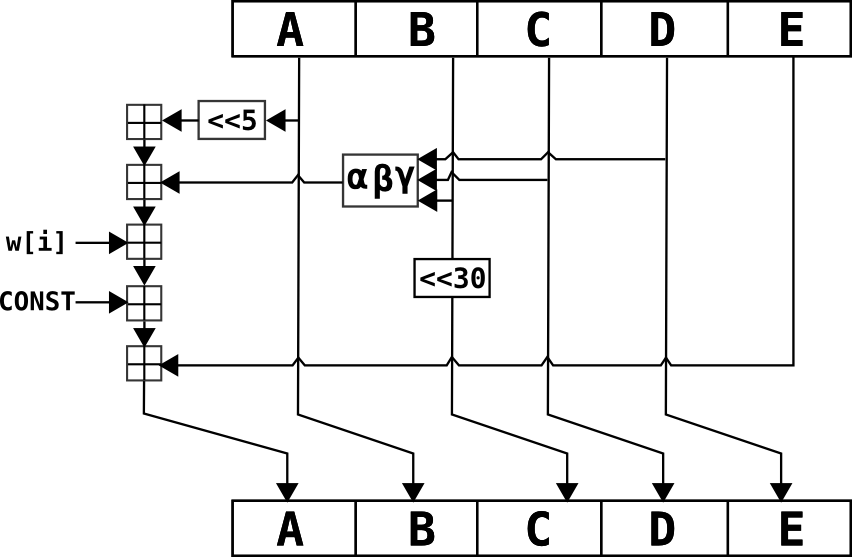
\includegraphics[scale=0.32]{figs/SHA1step.png}
	 \caption{Um passo do algoritmo SHA-1}
	\end{figure}

\begin{algorithm}
\caption{O algoritmo SHA-1}
\begin{algorithmic}
	\Require{Mensagem M}
	\Ensure{hash criptográfico de 160 \emph{bits}}
	\State $x \leftarrow$ \textbf{preenchimento\_mensagem}(M)
	\State $x = x_1 \| x_2 \| \ldots \| x_n$, onde cada $x_i$ é um bloco de 512 \emph{bits}
	\State Inicialização do estado $H$: 	$H_0^{(0)} \leftarrow \texttt{0x67452301}$, \hspace{2mm} $H_1^{(0)} \leftarrow \texttt{0xEFCDAB89}$, 
	\State \hspace{2mm} $H_2^{(0)} \leftarrow \texttt{0x98BADCFE}$, \hspace{2mm} $H_3^{(0)} \leftarrow \texttt{0x10325476}$ \hspace{2mm} $H_4^{(0)} \leftarrow \texttt{0xC3D2E1F0}$
	\For{(i=1, i< $n$, i++)}
		\State $x_i = w_0\|w_1\|\ldots\|w_{15}$, onde $w_i$ é uma palavra de 32 \emph{bits}
		\For{(j=16, j< 79, j++)}
			\State $w_j = (w_{j-3} \oplus w_{j-8} \oplus w_{j-14} \oplus w_{j-16}) \lll 1$
		\EndFor
		\State $a \leftarrow H_0^{(i-1)}, \hspace{2mm} b \leftarrow H_1^{(i-1)}, \hspace{2mm} c \leftarrow H_2^{(i-1)}, \hspace{2mm} d \leftarrow H_3^{(i-1)}, \hspace{2mm} e \leftarrow H_4^{(i-1)}$
		\For{(j=0, j< 19, j++)}
			\State $tmp \leftarrow (a \lll 5) + Ch(b,c,d) + e + w_j + \texttt{0x5A827999}$
			\State $e \leftarrow d$, \hspace{2mm} $d \leftarrow c$, \hspace{2mm} $c \leftarrow b \lll 30$, \hspace{2mm} $b \leftarrow a$, \hspace{2mm} $a \leftarrow tmp$
		\EndFor
		\For{(j=20, j< 39, j++)}
			\State $tmp \leftarrow (a \lll 5) + Parity(b,c,d) + e + w_j + \texttt{0x6ED9EBA1}$
			\State $e \leftarrow d$, \hspace{2mm} $d \leftarrow c$, \hspace{2mm} $c \leftarrow b \lll 30$, \hspace{2mm} $b \leftarrow a$, \hspace{2mm} $a \leftarrow tmp$
		\EndFor
		\For{(j=40, j< 59, j++)}
			\State $tmp \leftarrow (a \lll 5) + Maj(b,c,d) + e + w_j + \texttt{0x8F1BBCDC}$
			\State $e \leftarrow d$, \hspace{2mm} $d \leftarrow c$, \hspace{2mm} $c \leftarrow b \lll 30$, \hspace{2mm} $b \leftarrow a$, \hspace{2mm} $a \leftarrow tmp$
		\EndFor
		\For{(j=60, j< 79, j++)}
			\State $tmp \leftarrow (a \lll 5) + Parity(b,c,d) + e + w_j + \texttt{0xCA62C1D6}$
			\State $e \leftarrow d$, \hspace{2mm} $d \leftarrow c$, \hspace{2mm} $c \leftarrow b \lll 30$, \hspace{2mm} $b \leftarrow a$, \hspace{2mm} $a \leftarrow tmp$
		\EndFor
		\State $H_0^{(i)} \leftarrow a+H_0^{(i-1)}, \hspace{2mm} H_1^{(i)} \leftarrow b+H_0^{(i-1)}, \hspace{2mm} H_2^{(i)} \leftarrow c+H_2^{(i-1)}$,
		\State $H_3^{(i)} \leftarrow d+H_3^{(i-1)}, \hspace{2mm} H_4^{(i)} \leftarrow e+H_4^{(i-1)}$
	\EndFor
	\State \Return {$H_0^{(N)}\|H_1^{(N)}\|H_2^{(N)}\|H_3^{(N)}\|H_4^{(N)}$}	
\end{algorithmic}
\label{alg: Algoritmo SHA-1}	
\end{algorithm} 

\subsection{SHA-2}

O algoritmo \textit{SHA-2}, projetado com uma estrutura similar ao \textit{SHA-1}, processa mensagens de até $2^{128}$ e produz
hashes de $224$, $256$, $384$ e $512$ bits. 
Os algoritmos \textit{SHA-224} e \textit{SHA-384} são idênticos aos algoritmos \textit{SHA-256} e \textit{SHA-512}, respectivamente, apenas sofrendo um truncamento do valor do hash gerado. 
A função de compressão do \textit{SHA-26} recebe  como entrada um bloco de mensagem de $512$ bits e um bloco de hash de $256$ bits e gera como saída um hash de $256$ bits. 
A função de compressão do \textit{SHA-512}, recebe um bloco de mensagem de $1024$ bits e um bloco de hash de $512$ bits e gera uma sáida de $512$ bits. 
A seguir descreveremos a versão \textit{SHA-256}, para mais detalhes do algoritmo \textit{SHA-2} consultar \cite{NIST2008}.

\noindent No algoritmo ~\ref{alg:INIT_SHA-2} a mensagem será dividida em blocos e as variáveis do hash inicial serão inicializadas. 
A etapa de preenchimento da mensagem é idêntica ao algoritmo \textit{SHA-1}. 
	\begin{algorithm}
	\caption{Inicialização SHA-256}
	\begin{algorithmic}
	\Require{Mensagem M}
	\Ensure{Mensagem M dividida em blocos e variável de estado inicializado}
	\State $x \leftarrow$ \textbf{preenchimento\_mensagem}(M)
	\State $x = x_1 \| x_2 \| \ldots \| x_n$, onde cada $x_i$ é um bloco de 512 \emph{bits}
	\State Seja o hash $H$ inicializado da seguinte forma,
	\State $H_0^{(0)} \leftarrow \texttt{0x6A09E667}$
	\State $H_1^{(0)} \leftarrow \texttt{0xBB67AE85}$
	\State $H_2^{(0)} \leftarrow \texttt{0x3C6Ef372}$
	\State $H_3^{(0)} \leftarrow \texttt{0xA54FF53A}$
	\State $H_4^{(0)} \leftarrow \texttt{0x510E527F}$
	\State $H_5^{(0)} \leftarrow \texttt{0x9B05688C}$
	\State $H_6^{(0)} \leftarrow \texttt{0x1F83D9AB}$
	\State $H_7^{(0)} \leftarrow \texttt{0x5BE0CD19}$
	\State \Return{$H$, e $x$}
\end{algorithmic}
\label{alg:INIT_SHA-2}	
\end{algorithm} 

O \textit{SHA-256} usa seis funções internas, sendo duas idênticas às funções usadas no \textit{SHA-1}:

	1. $Ch(x,y,z) = (x \wedge y) \oplus (\neg(x) \wedge z);$

	2. $Maj(x,y,z) = (x \wedge y) \oplus (x \wedge z) \oplus (y \wedge z);$

	3. $\sum_0^{\{256\}}(x) = (x \ggg 2) \oplus (x \ggg 13) \oplus (x \ggg 22);$

	4. $\sum_1^{\{256\}}(x) = (x \ggg 6) \oplus (x \ggg 11) \oplus (x \ggg 25);$

	5. $\sigma_0^{\{256\}}(x) = (x \ggg 7) \oplus (x \ggg 18) \oplus (x \gg 3);$

	6. $\sigma_1^{\{256\}}(x) = (x \ggg 17) \oplus (x \ggg 19) \oplus (x \gg 10).$

	Assim como no \textit{SHA-1}, o bloco da mensagem de $512$ bits será dividido em $16$ palavras de $32$ bits, uma expansão é feita, resultando em $64$ palavras de $32$ bits. 
	Em seguida, $64$ rodadas são aplicadas, porém, no \textit{SHA-2}, cada rodada utilizará uma constante distinta. 
	Ao final, as variáveis do hash  inicial são adicionadas ao valor gerado em cada rodada.
	\begin{algorithm}
	\caption{SHA-256}
	\begin{algorithmic}
	\Require{Mensagem $M$ dividida em $n$ blocos de 512 bits e variáveis do hash  ini\-cializadas}
	\Ensure{hash criptográfico de 256 bits}
	\For{(i=1,i< $n$,i++)}
		\State $x_i = w_0\|w_1\|\ldots\|w_{15}$, onde cada $w_i$ é uma palavra de 32 \emph{bits}
		\State Expansão da mensagem
		\For{(j=16, j< 63, j++)}
			\State $w_j = \sigma_1^{\{256\}}(w_{t-2}) + w_{t-7} + \sigma_0^{\{256\}}(w_{t-15}) + w_{t-16}$
		\EndFor
		\State Guardar valores iniciais do estado
		\State $a \leftarrow H_0^{(i-1)}, \hspace{2mm} b \leftarrow H_1^{(i-1)}, \hspace{2mm} c \leftarrow H_2^{(i-1)}, \hspace{2mm} d \leftarrow H_3^{(i-1)},$
		\State $e \leftarrow H_4^{(i-1)}, \hspace{2mm} f \leftarrow H_5^{(i-1)}, \hspace{2mm} g \leftarrow H_6^{(i-1)}, \hspace{2mm} h \leftarrow H_7^{(i-1)}$ 
		\For{(j=0, j< 63, j++)}
			\State $tmp_1 \leftarrow h + \sum_1^{\{256\}}(e) + Ch(e,f,g) + CONST_j + w_j$
			\State $tmp_2 \leftarrow \sum_0^{\{256\}}(a) + Maj(a,b,c)$
			\State $h \leftarrow g$
			\State $g \leftarrow f$
			\State $f \leftarrow e$
			\State $e \leftarrow d + tmp_1$
			\State $d \leftarrow c$
			\State $c \leftarrow b$
			\State $b \leftarrow a$
			\State $a \leftarrow tmp_1 + tmp_2$
		\EndFor	
		\State $H_0^{(i)} \leftarrow a+H_0^{(i-1)}, \hspace{2mm} H_1^{(i)} \leftarrow b+H_1^{(i-1)}, \hspace{2mm} H_2^{(i)} \leftarrow c+H_2^{(i-1)}, \hspace{2mm} H_3^{(i)} \leftarrow d+H_3^{(i-1)},$
		\State $H_4^{(i)} \leftarrow e+H_4^{(i-1)}, \hspace{2mm} H_5^{(i)} \leftarrow f+H_5^{(i-1)}, \hspace{2mm} H_6^{(i)} \leftarrow g+H_6^{(i-1)}, \hspace{2mm} H_7^{(i)} \leftarrow h+H_7^{(i-1)}$
	\EndFor
	\State \Return {$H_0^{(N)}\|H_1^{(N)}\|H_2^{(N)}\|H_3^{(N)}\|H_4^{(N)}\|H_5^{(N)}\|H_6^{(N)}\|H_7^{(N)}$}
\end{algorithmic}
\label{alg: Algoritmo SHA-2 (256)}	
\end{algorithm} 

\vspace*{5mm}
\begin{figure}[H]  
  \centering 
  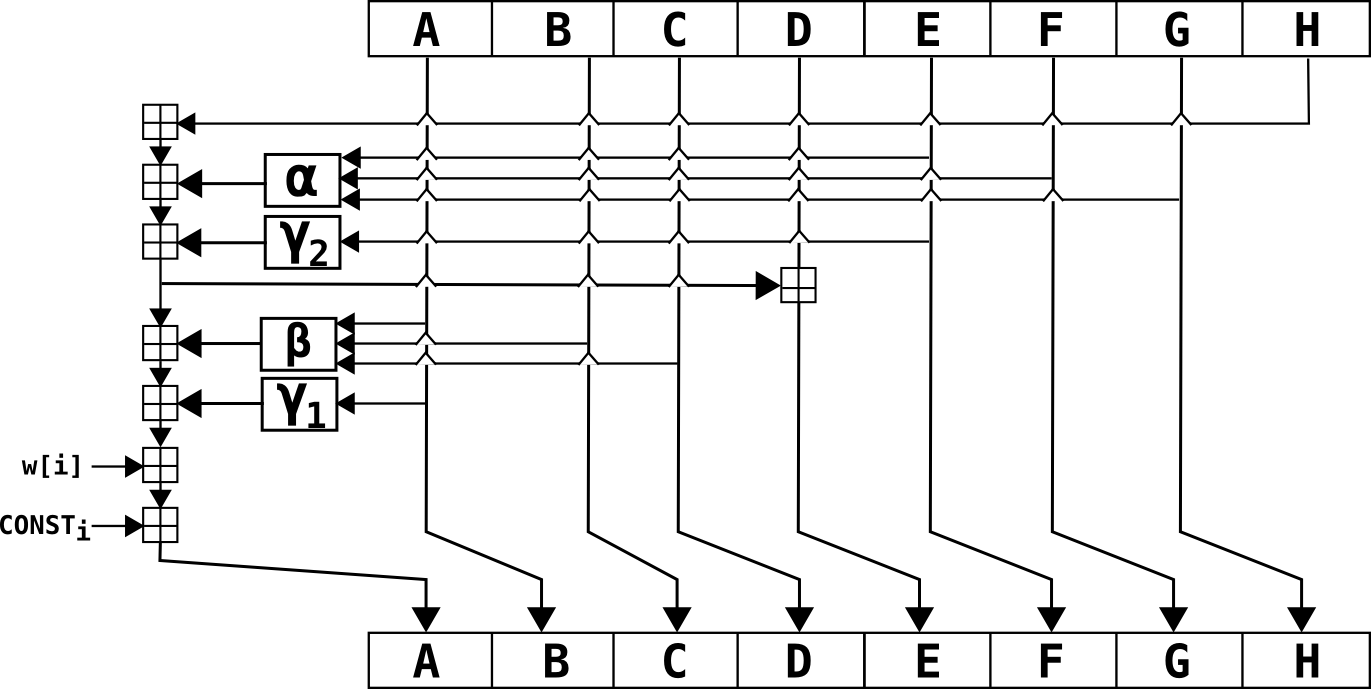
\includegraphics[scale=0.35]{figs/SHA2step.png}
 \caption{Um passo do algoritmo SHA-2}
\end{figure}

}
%
\subsection{Esquemas de Assinatura}
Um esquema de assinatura $SIGN$ é uma tripla de algoritmos: $(GEN;SIG;VER)$ que satisfaz as seguintes propriedades:
\begin{enumerate}
\item O algoritmo de geração de chaves $GEN$ recebe como entrada um parâmetro de seguranca $1^n$ e produz  um
      par de chaves $(X,Y)$, onde $X$ é  a chave privada e $Y$ é a chave pública.
\item O algoritmo de geração de assinatura $SIG$ recebe como entrada uma mensagem  $M \in \{0,1\}^{*}$ e uma chave privada $X$ e produz uma assinatura $Sig$, denotada por $ Sig \leftarrow SIG_{X}(M)$.
\item O algoritmo de verificação de assinatura $VER$ recebe como entrada uma mensagem $M$, uma assinatura $Sig$ de $M$
      e uma chave pública $Y$ e produz um bit $b$, onde $b=1$ significa que a assinatura é válida e $b=0$ indica que a assinatura é inválida.
\end{enumerate}
\subsection{Assinatura one-time}\label{onetime}
Assinaturas One-Time aparecem inicialmente nos trabalhos Lamport~\cite{lamport:79} e Rabin~\cite{Rabin78}. Merkle~\cite{merkle:79} propôs uma técnica que permite transformar um esquema de assinaturas \textit{one-time} em um esquema com número de assinaturas arbitrário. A seguir descreveremos os esquemas de Lamport~\cite{lamport:79} e Winternitz~\cite{merkle:87}.

\subsubsection{Esquema de assinatura one-time de Lamport:}

O esquema de assinatura \textit{one-time} de Lamport \textit{(LD-OTS)} foi proposto em~\cite{lamport:79}. 
Seja $n$ um inteiro positivo, o parâmetro de segurança, o esquema \textit{LD-OTS} utiliza uma função \textit{one-way} 
$$f:\{0,1\}^{n}  \to \{0, 1\}^{n} $$
e uma função de hash criptográfico 
$$g:\{0, 1\}^*  \to \{0, 1\}^n.$$
\newline \newline \textit{Geração do par de chaves LD-OTS}: A chave de assinatura $X$ consiste de $2n$ cadeias de bits de comprimento $n$ escolhidos aleatoriamente,
$$X = (x_0[0],x_0[1],...,x_{n-1}[0],x_{n-1}[1]) \quad \in \quad _R\{0,1\}^{(n,2n)}. $$
A chave de verificação $Y$ é
$$Y = (y_0[0],y_0[1],...,y_{n-1}[0],y_{n-1}[1]) \quad  \in \quad \{0,1\}^{(n,2n)}. $$
onde $y_i[j]=f(x_i[j])$, $0 \le i \le {n-1}$, $j=0,1$.  
\newline \newline \textit{Geração de assinatura LD-OTS}: O hash $d$ de uma mensagem $M$ é assinada u\-sando a chave de assinatura $X$.
Para assinar, primeiro calcula-se $d=g(M)=(d_{0},...,d_{n-1})$. Então, o assinante gera a assinatura
$$ Sig=(sig_0,...,sig_{n-1})=(x_0[d_0],...,x_{n-1}[d_{n-1}])\quad  \in \quad \{0,1\}^{(n,n)}.$$
Para gerar $Sig$, não há aplicações da função de hash, pois a assinatura realiza somente a seleção de bits da chave $X$ de acordo com os bits do hash da mensagem.
\newline \newline \textit{Verificação de assinatura LD-OTS}: Na verificação de assinatura, o verificador tem como entrada: a assinatura $Sig=(sig_{0},...,sig_{n-1})$, a mensagem $M$ e a correspondente chave pública de verificação $Y$.
Para verificar, primeiro calcula-se o hash da mensagem $d=g(M)=(d_{0},...,d_{n-1})$. Então o verificador checa se
$$ Sig=(f(sig_{0}),...,f(sig_{n-1})) = (y_0[d_0],...,y_{n-1}[d_{n-1}]).$$

Na Figura ~\ref{fig:lamport} ilustramos o esquema de Lamport. Neste exemplo a função \textit{one-way} utilizada foi $f(x)= x+1$ mod $16$.
Para a geração da chave de verificação, são necessárias $2n$ aplicações da função \textit{one-way}, uma para cada elemento de $X$. 
Para a verificação da assinatura, a função \textit{one-way} é executada $n$ vezes, uma para cada elemento de $Sig$.

\begin{figure}[htbp] \centering
    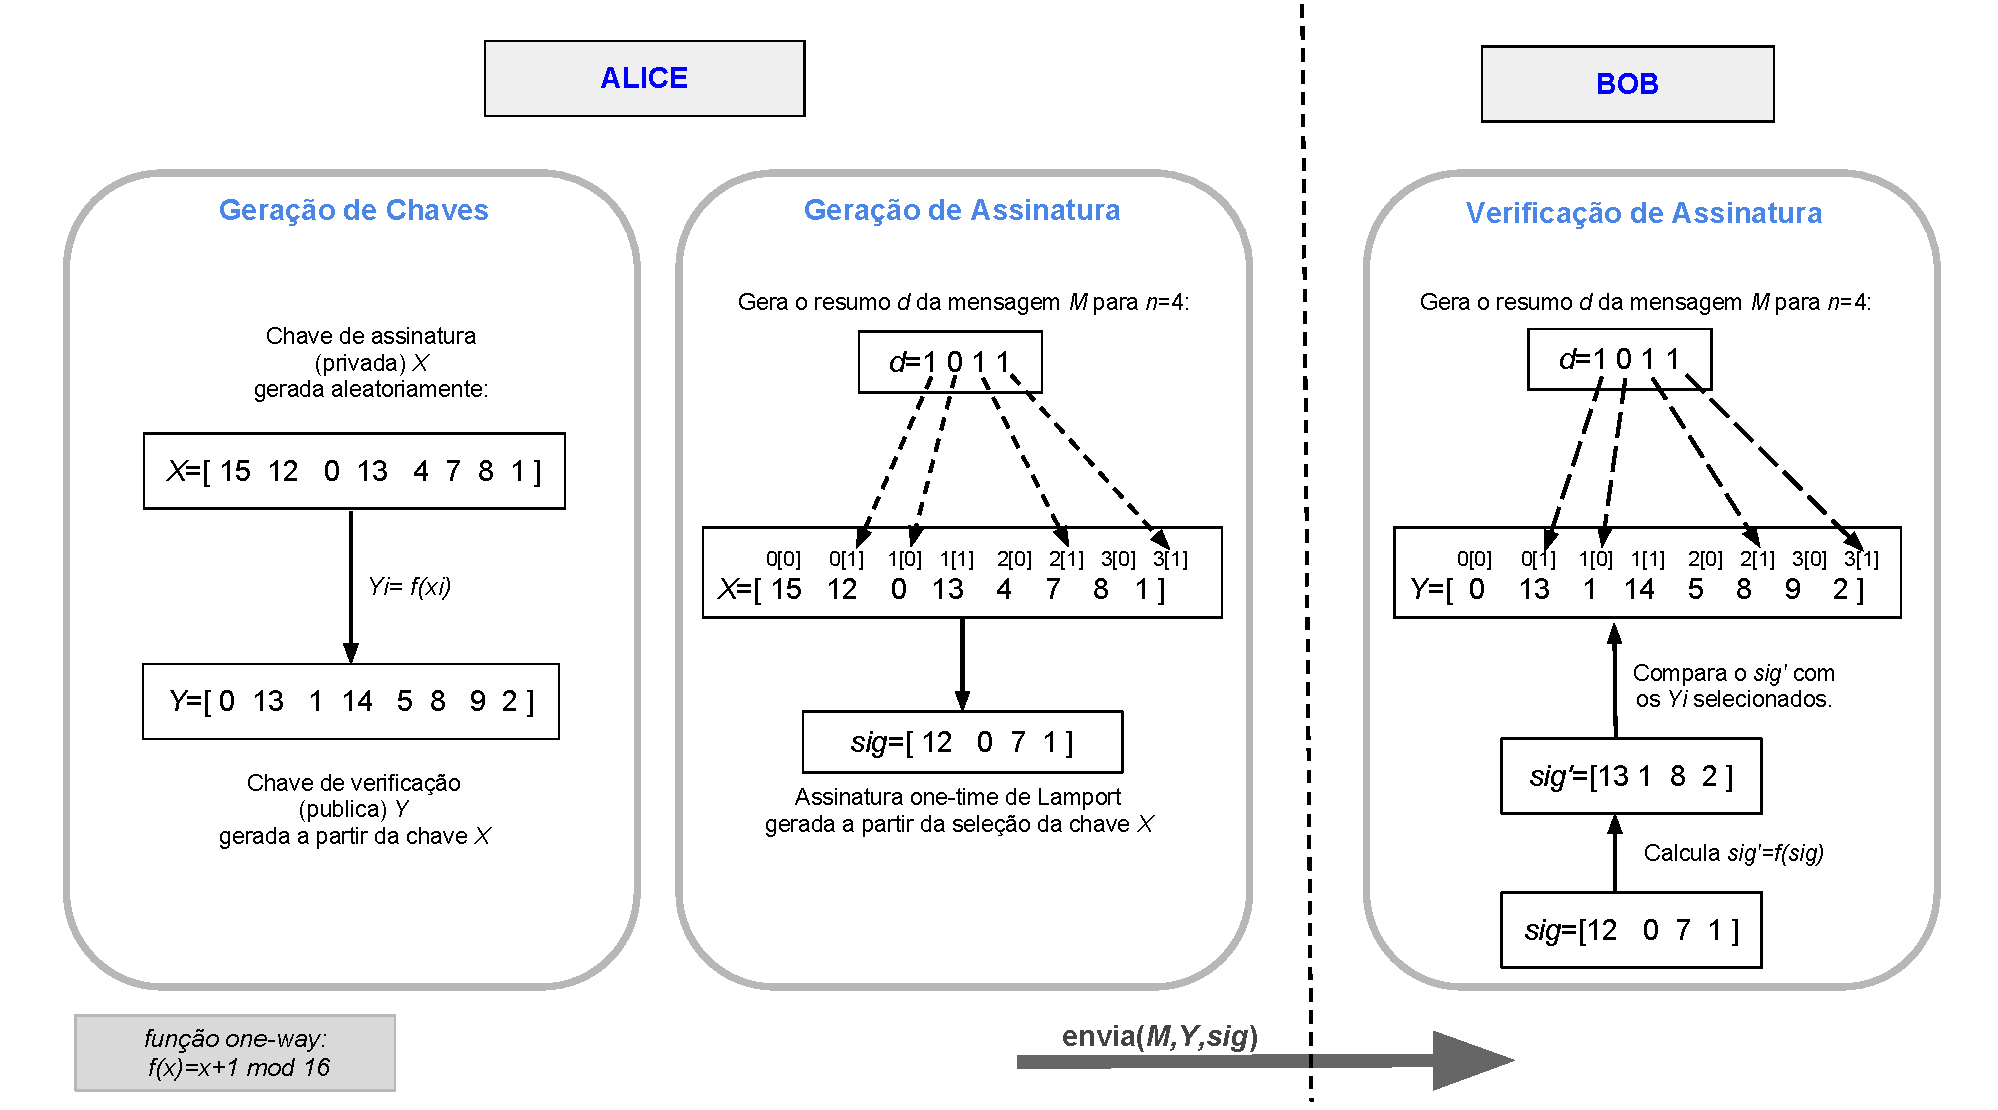
\includegraphics[scale=0.4]{figs/Lamport.pdf}
\caption{Exemplo do esquema de assinatura \textit{one-time} de Lamport }
\label{fig:lamport}
\end{figure}

\subsubsection{Esquema de assinatura \textit{one-time} de Winternitz:}

Winternitz propôs uma melhora no esquema de assinatura \textit{one-time} de Lamport, diminuindo o tamanho da chave pública e privada. 
Este esquema \textit{W-OTS} foi mencionado pela primeira vez em ~\cite{merkle:87}.
O esquema \textit{W-OTS} utiliza uma função \textit{one-way} 
$$f:\{0,1\}^{n}  \to \{0, 1\}^{n} $$
e uma função de hash criptográfica 
$$g:\{0, 1\}^*  \to \{0, 1\}^n,$$ onde $n$ é um inteiro positivo.
O parâmetro $w$ denota o número de bits que são processados simultaneamente.  Quanto maior for o $w$ menor será a chave de assinatura e maior será o tempo de assinatura e verificação. 
Em ~\cite{dods:05} foi feita uma análise comparativa do tempo de execução e tamanho das chaves em relação ao parâmetro $w$.
\newline \newline \textit{Geração do par de chaves {W-OTS}}: Um parâmetro $w \in$ $\mathbb{N}$ é escolhido.  A chave de assinatura privada é 
$$ X=(x_0, ..., x_{t-1}) \in_\mathcal{R} \{0,1\}^{(n,t)}$$
onde os $x_i$ são escolhidos aleatoriamente. 
O tamanho $t$ é obtido calculando $t=t_1+t_2$, onde 
$$ t_1= \Bigg \lceil \frac {n}{w}\Bigg\rceil,   \qquad t_2=\Bigg\lceil \dfrac{\lfloor log_2 t_1 \rfloor +1+w}{w}\Bigg\rceil .$$
A chave pública de verificação 
$$ Y=(y_0,...,y_{t-1})  \in \{0,1\}^{(n,t)}$$
é gerada aplicando a função $f$ a cada elemento da chave de assinatura $2^w-1$ vezes:  
$$ y_i=f^{2^{w}-1} (x_i),  \qquad para \quad i=0,...,t-1. $$

Na Figura ~\ref{fig:genKeyWinternitz} mostramos um exemplo do processo de geração de chaves para o esquema de assinatura de Winternitz, utilizando uma função \textit{one-way}. 
Este esquema produz chaves de assinaturas menores que o de Lamport, porém aumenta o número de aplicação da função \textit{one-way} de $1$ para $2^w-1$ em cada elemento da chave de assinatura.
\begin{figure}[htbp] \centering
    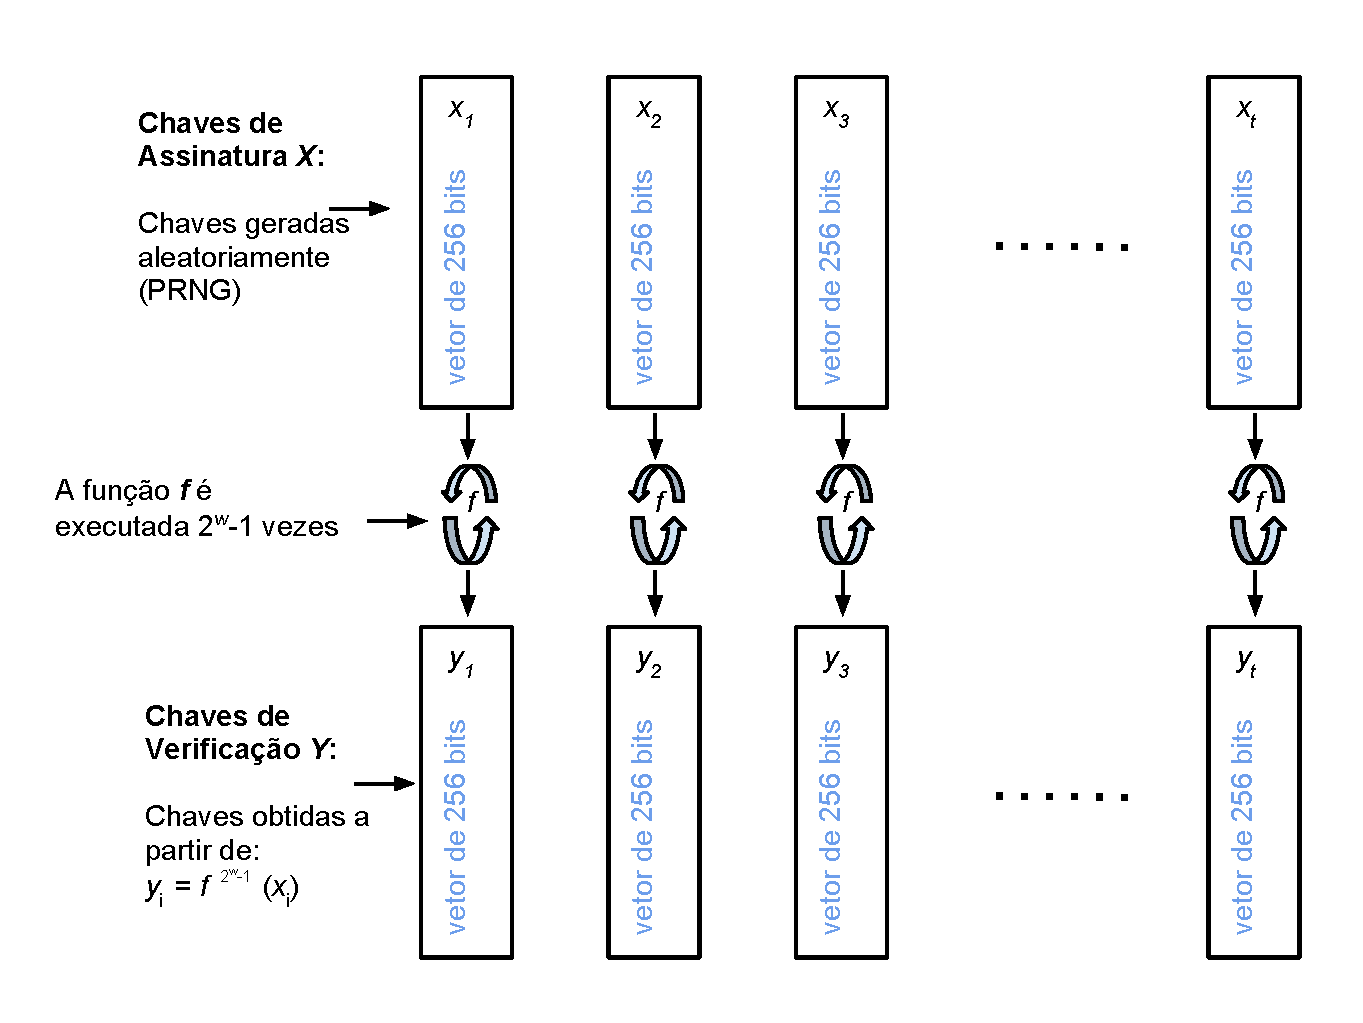
\includegraphics[scale=0.4]{figs/genKeyWintern.pdf}
\caption{Exemplo da geração de chaves no esquema de assinatura \textit{one-time} de Winternitz }
\label{fig:genKeyWinternitz}
\end{figure}
\newline\newline \textit{Geração de assinatura W-OTS}: Para gerar uma assinatura, primeiro calcula-se o hash da mensagem $d=g(M)=(d_0,...,d_{n-1})$. 
Se necessário, adicionamos zeros a esquerda de $d$, tal que $d$ seja divisível por $w$.
Então $d$ é dividido em $t_1$ blocos binários de tamanho $w$, resultando em $d=(m_{0} || ...|| m_{t_1-1})$, onde $||$ representa a concatenação. 
Os blocos $m_i$  são representados como inteiros em $\{0,1,...,2^w-1\}$. Então calcula-se o checksum 
$$ c=\sum_{i=0}^{t_1-1}  (2^w-m_i).$$
Como  $c \leq t_1 2^w$, o comprimento da representação binária de $c$ é menor que $\lfloor \log_2 t_1 2^w\rfloor + 1 = \lfloor \log_2 t_1\rfloor + w + 1$.
Se for necessário, adicionam-se zeros à esquerda do $c$ de tal forma que a cadeia $c$ estendida seja divisível por $w$. 
Então a cadeia estendida $c$ pode ser dividida em $t_2$ blocos $c=(c_0||\ldots||c_{t_2-1})$ de comprimento $w$. 
Concatenamos em $b$ a cadeia estendida $d$ com a cadeia estendida $c$.
Então $b=(b_{0}||b_{1}||\ldots||b_{t-1})=(m_{0} || \ldots || m_{t_1-1}||c_{0}|| \ldots|| c_{t_2-1})$.
Calculamos a assinatura como:
$$ Sig=(sig_0,...,sig_{t-1})=(f^{b_0}(x_0), f^{b_1}(x_1),...,f^{b_{t-1}}(x_{t-1})). $$
\textit{Verificação de assinatura W-OTS}: Para verificar a assinatura $Sig=(sig_{0},...,sig_{t-1})$ da mensagem $M$, primeiro calculamos os parâmetros $b_{0},...,b_{t-1}$ da mesma forma que durante a geração de assinatura. 
Depois, calcula-se:
$$ sig'_i=f^{2^w-1-b_i}(sig_i), \qquad para \quad i=0,...,{t-1}. $$
Então, para checar a assinatura, verifica:
\newline se $Sig’=(sig'_0,\ldots,sig’_{t-1})$ é igual a $Y=(y_0,\ldots,y_{t-1})$ a assinatura é válida, caso contrário é recusada.

\subsection{MSS-Esquema de assinatura digital de Merkle}\label{merkle}

No esquema de assinatura digital de Merkle descrito a seguir, a chave de assinatura e a chave de verificação \textit{one-time} são as folhas da árvore e, a chave pública, é a raiz. 
Uma árvore com altura $H$ e $2^H$ folhas terá $2^H$ pares de chaves \textit{one-time} públicas e privadas.

\subsubsection{Geração de chaves da árvore de Merkle}

Para gerar a chave pública \textit{pub} de Merkle, que corresponde a raiz da árvore de Merkle, primeiro é preciso gerar o par de chaves, pública e privada, \textit{one-time} para cada folha da árvore de Merkle.
\newline \newline \textit{Geração do par de chaves {one-time}}: Um algoritmo de assinatura \textit{one-time} gera as chaves privadas $X[u]$ e públicas $Y[u]$, para as folhas $u=1,...,2^H$.
O Algoritmo ~\ref{genKey} descreve o processo de ge\-ração de um par de chaves \textit{one-time} de Winternitz. 
Um algoritmo de geração de números pseudo-aleatórios \textit{PRNG} é utilizado para gerar os $t$ elementos da chave de assinatura, reduzindo o custo de armazenamento das chaves privadas, pois somente a semente do \textit{PRNG} é armazenada.

\begin{algorithm}
\caption{Geração do par de chaves \textit{one-time} de Winternitz~\cite{merkle:79}}
\begin{algorithmic}
\Require parâmetro Winternitz t.
\Ensure Matrizes X, Y de tamanho[$2^H$][256].
\State Cria as matrizes X e Y.
\State Cria as matrizes temporárias x e y de tamanho[t][256].
\For{($u =1$, $u < t$, u++)}
	\State Gera aleatoriamente a semente para o PRNG: $X[u]=semente$;
	\State x[0]=$PRGN(X[u]);$
	\For{($i =1$, $i < t$, i++)}
	    \State y[i-1] = $f^{2^{w}-1}(x[i-1]);$		
	    \State x[i] = $PRNG(x[i-1]);$
	\EndFor
	\State Y[u]=$g(y[0]|| ...|| y[t-1]);$
	\State \Return X,Y;
\EndFor
\end{algorithmic}
\label{genKey}
\end{algorithm} 

\noindent \textit{Geração da chave pública pub}: O Algoritmo ~\ref{arvoreHash} gera a chave pública \textit{pub} da árvore de Merkle. 
Os valores de entrada são: a folha inicial $folhaIni$ e a altura da árvore $alturaMax$.
Cada nó folha $(no[u])$ da árvore, recebe a chave de verificação $(Y[u])$ daquela folha. 
O valor de cada nó intermediário $(no[pai])$ é o resultado da aplicação da função de hash na concatenação dos valores de seus dois filhos, esquerdo $(no[esq])$ e direito $(no[dir])$. 
Cada vez que uma folha $u$ é calculada e empilhada em $pilhaNo$, o algoritmo verifica se os nós do topo da pilha tem alturas iguais. 
Se as alturas forem iguais, os dois nós serão desempilhados, concatenados em $no[pai]$ e gerado um novo hash, que será empilhado em $pilhaNo$. 
O algoritmo termina quando a raiz da árvore é encontrada.

\begin{algorithm}
\caption{ArvoreDehash~\cite{merkle:79}}
\begin{algorithmic}
\Require Inteiros folhaIni, alturaMax; Matrizes de 256 bits Y;
\Ensure Uma estrutura nó pub: A raiz da árvore. 
\State Cria uma pilha $pilhaNo$.
\For {($u =folhaIni$, $u < 2^{alturaMax}$, u++)}
      \State Guarda Y[u] em nó folha $no[u].hash=(Y[u])$
      \State Empilha $no[u]$ na pilha $pilhaNo$
      \While {Os nós do topo da pilha $pilhaNo$ tiverem altura iguais}
	  \State Desempilha o nó $no[dir]$ de $pilhaNo$
	  \State Desempilha o nó $no[esq]$ de $pilhaNo$
	  \State Calcula $no[pai].hash=g(no[esq].hash||no[dir].hash)$
	  \If {$no[pai].altura$=$alturaMax$ }
	      \State \Return $(no[pai])$		
	  \Else
	      \State Empilha $no[pai]$ na pilha $pilhaNo$
	  \EndIf
      \EndWhile
\EndFor
\end{algorithmic}
\label{arvoreHash}
\end{algorithm}

A Figura ~\ref{fig:treehash} demonstra a ordem em que os nós são empilhados na árvore conforme execução do Algoritmo ~\ref{arvoreHash}.
Os nós em cinza, representam os nós que já foram gerados. O $4^o$ nó da árvore gerado (folha $u=2$), recebeu o valor de $Y[2]$. 
O $3^o$ nó é resultado do hash da concatenação dos nós 1 e 2.

\begin{figure}[htbp] \centering
    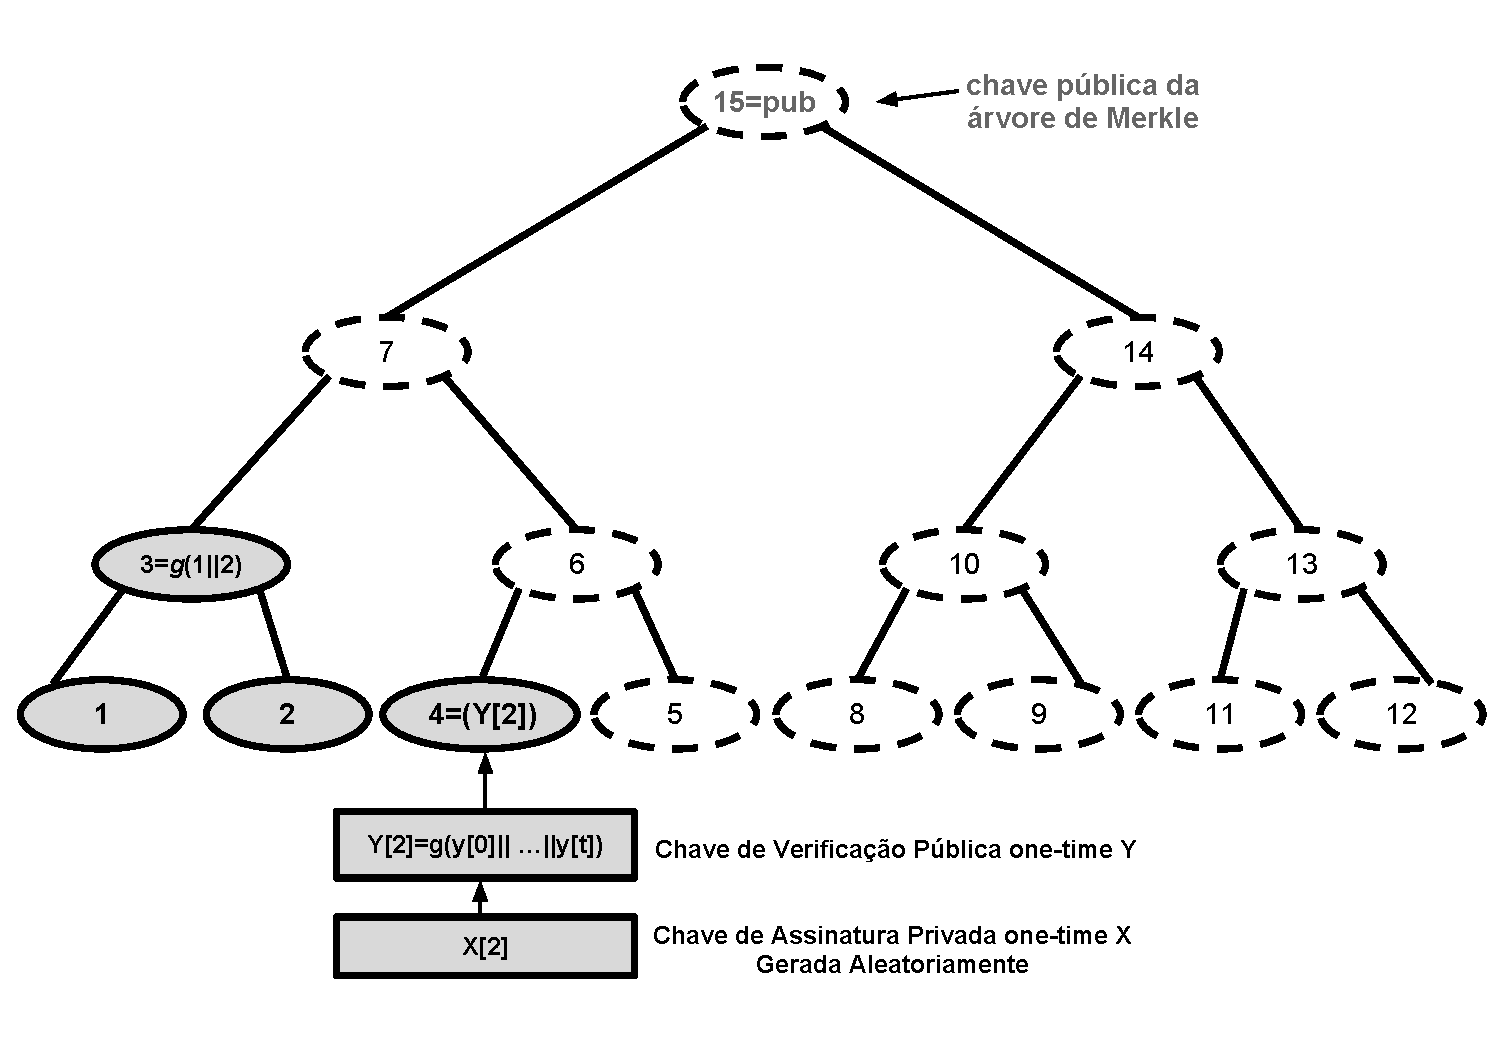
\includegraphics[scale=0.4]{figs/treehash.pdf}
\caption{Geração da chave pública da árvore de Merkle }
\label{fig:treehash}
\end{figure}

\subsubsection{Geração de assinatura} O esquema \textit{MSS} permite a geração de $2^H$ assinaturas, para uma árvore de altura $H$.
Suponha que tenhamos $M[u]$ mensagens, para $u=0,..,2^H$. A mensagem $M[u]$ é assinada com o esquema de assinatura \textit{one-time}, resultando em uma assinatura $Sig$, no qual utiliza a chave $X[u]$ para assinar a mensagem $M[u]$, conforme apresentado em~\cite{bernst:09}. 
Uma árvore de autenticação $Aut$ é utilizada para guardar os nós no ca\-minho necessários para autenticar uma folha $Y[u]$, reduzindo a necessidade de enviar toda a árvore para o receptor. 
A assinatura $SIG$ de Merkle é composta de $Sig$ e da cor\-respondente chave de verificação $Y[u]$. Também é preciso incluir o índice $u$ (índice da folha) e o respectivo caminho de autenticação, $Aut=(Aut[0],..,Aut[H-1])$. 
Assim, a assinatura $SIG=(u, Sig,Y[u],(Aut[0],...,Aut[H-1]))$. 

\noindent \textbf{O algoritmo clássico do caminho de autenticação.} O algoritmo clássico do caminho de autenticação \textit{(Classic Merkle Tree Traversal)} ~\cite{merkle:87} calcula os nós de autenticação $Aut$ para cada folha da árvore, necessários para autenticar a chave pública $pub$ da árvore de Merkle.
Este algoritmo utiliza duas variáveis do tipo pilha: $Aut$ e $Aux$. 
A pilha $Aut$ contém o caminho de autenticação atual e a pilha $Aux$ guarda os próximos nós de autenticação que serão necessários. 
O caminho $Aut$ é composto pelos valores dos nós $Aut[h]$ em cada altura que são os irmãos direitos dos nós no caminho de autenticação que ligam a folha até a raiz da árvore de Merkle. 

Vamos descrever o processo de geração dos caminhos de autenticação.
O primeiro caminho de autenticação é gerado durante a execução do Algoritmo ~\ref{arvoreHash}.
Os próximos caminhos de autenticação são gerados pelo Algoritmo ~\ref{algTraversal} a medida em que as assinatura são realizadas.
Na Figura~\ref{traversal}, os nós em cinza mostram o primeiro caminho de autenticação $Aut$ para a folha $u=0$.


\begin{figure}[htbp] \centering
  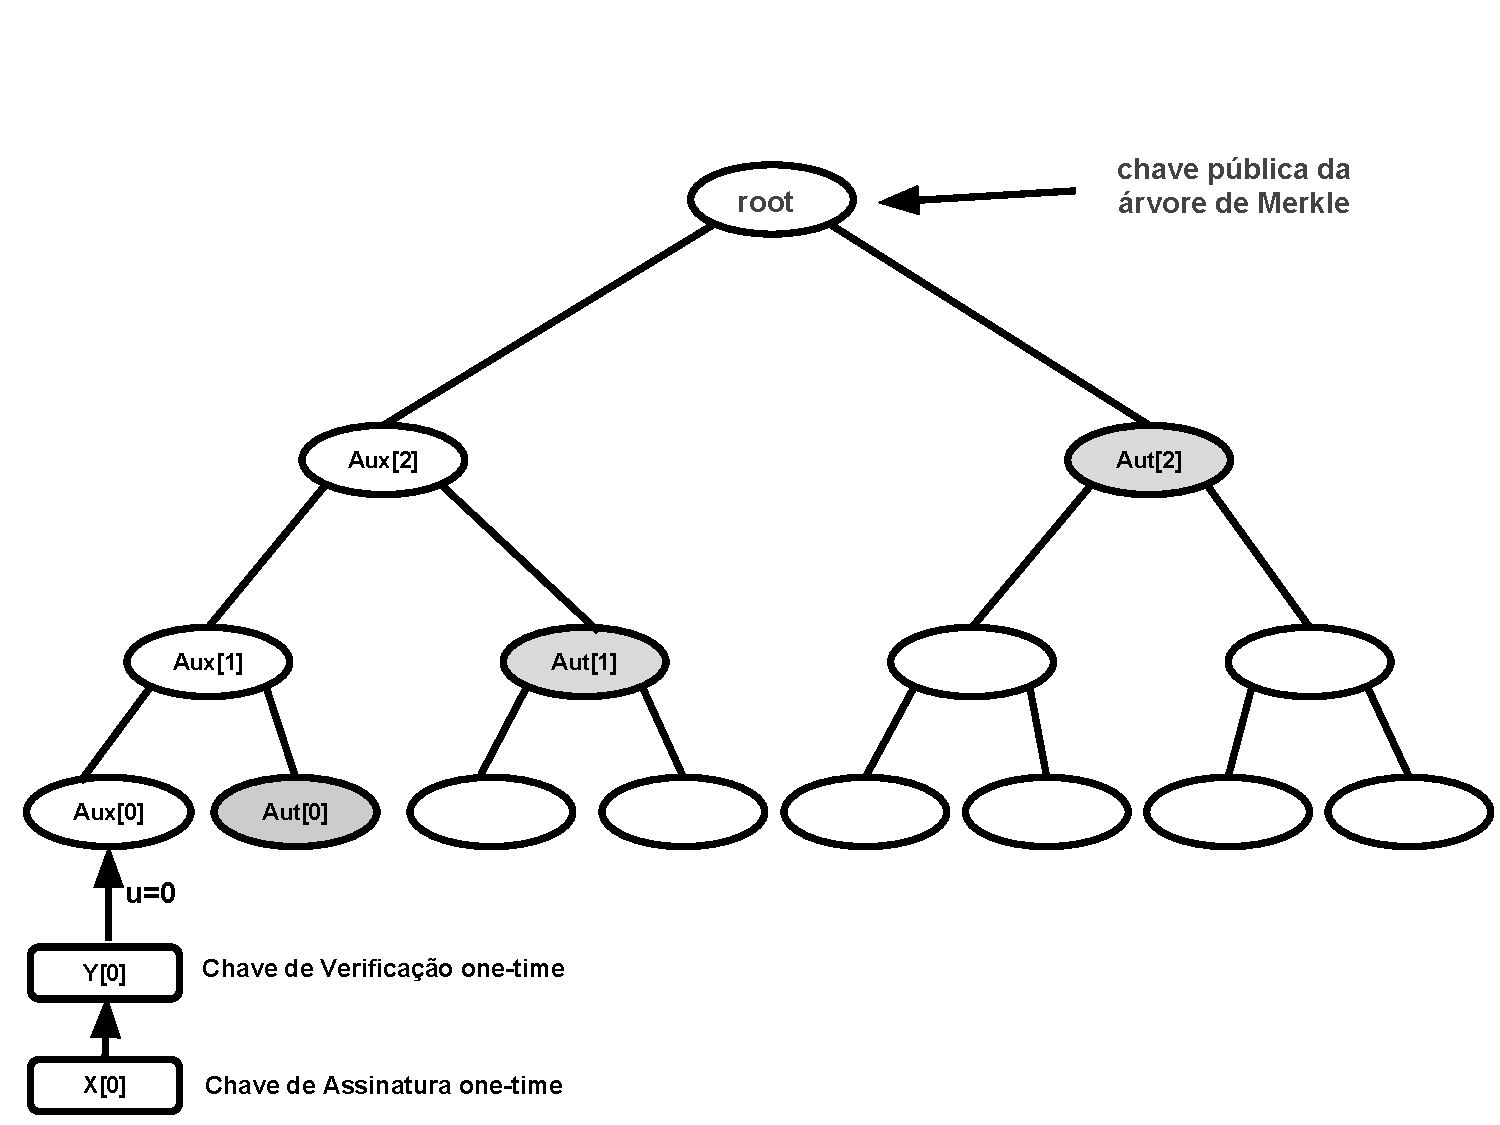
\includegraphics[scale=0.4]{figs/traversal.pdf}
\caption{Execução do Algoritmo ~\ref{arvoreHash} com o primeiro caminho de autenticação}.
\label{traversal}
\end{figure}

\noindent \textbf{Fase de saída e atualização.} O Algoritmo~\ref{algTraversal} mostra os passos para produzir o próximo caminho de autenticação para a folha $u$ seguinte na árvore. 
A primeira assinatura usa a folha $u=0$ e a cada assinatura realizada, a folha é atualizada em uma unidade e o próximo caminho de autenticação é preparado de forma eficiente, pois somente os nós do caminho que mudam serão atualizados. 

\begin{algorithm}
\caption{Algoritmo de percurso na árvore~\cite{merkle:79}}
\begin{algorithmic}
\Require Inteiro altura $H$.
\Ensure Uma assinatura com o caminho de autenticação: $Aut$. 
\For {($u =0$, $u<2^{H}$, $u++$)}
	\For {($ h=0, h< H, h++$)}
	  \Return A pilha $Aut$ da folha $u$
	\EndFor
	\State O assinante assina com a folha $u$
	\For {($ h=0, h< H, h++$)}
	  \If {$(u+1)/(2^h)=0$}
	    \State Atualiza $Aut[h]=Aux[h]$
	    \State $no_{Ini}=(u+1+2^h) \oplus 2^h$.	    
	    \State $Aux[h].atualiza(no_{Ini}, h)$.
	  \EndIf
	\EndFor
\EndFor
\end{algorithmic}
\label{algTraversal}
\end{algorithm}

O Algoritmo~\ref{algTraversal} atualiza os nós de autenticação através da execução da função $Aux[h].atualiza(no_{Ini}, h)$, que executa o Algoritmo ~\ref{arvoreHash} no nó e altura selecionados. 
Depois de $2^h$ rodadas o valor do nó selecionado será completado.

\subsubsection{Verificação de assinatura} De acordo com o método em ~\cite{bernst:09}, o processo de verificação de assinatura consiste de duas etapas: na primeira etapa, a assinatura $Sig$ é verificada utilizando-se a chave de verificação \textit{one-time} $Y[i]$ e o res\-pectivo algoritmo \textit{one-time}; na segunda etapa, é preciso validar a chave pública da árvore de Merkle, então o receptor calcula o respectivo caminho de autenticação, construindo o caminho $(p[0],...,p[H])$ da folha $i$ até a raiz, para toda altura $h$. O índice $i$ é utilizado para decidir em qual ordem o ca\-minho de autenticação será recons\-truído. 
Inicialmente, para a folha de índice $i$, $p[0]=g(Y[i])$. Para $h=1,2,\ldots,H$ executa-se a condição a seguir para calcular o valor hash da sequência dos nós em cada altura:
\[ p[h]  = \left \{  \begin{array}{ll}
 g( Aut[h-1] \| p[h-1] )& \mbox{if $ \lfloor i/(2^{h-1})\rfloor \equiv 1 \ \rm{mod}\ 2 $;} \\

g(p[h-1] \| Aut[h-1])  & \mbox{caso contário.}
\end{array}
\right. \]
Ao final, compara-se o valor de $p[H]$ com a chave pública conhecida $pub$. Se o valor for igual, a autenticação é confirmada.

\subsection{CMSS - Um aperfeiçoamento no esquema de assinatura de Merkle}
O esquema \textit{CMSS}~\cite{buch:06}  é uma variante do esquema \textit{MSS} que permite aumentar a quantidade de assinaturas de $2^{20}$ para $2^{40}$. 
Neste trabalho os autores demons\-traram que \textit{CMSS} é competitivo na prática, apresentando uma aplicação altamente eficiente dentro do \textit{Java Cryptographic Service Provider FlexiProvider} e mostraram que a aplicação pode ser usada para assinar mensagens no Microsoft Outlook.

No esquema \textit{CMSS} são construídas duas árvores, uma subárvore e uma árvore principal, cada uma com $2^h$ folhas, para $h=H/2$. 
Assim, aumenta o número de assinaturas em relação ao \textit{MSS}, pois o \textit{MSS} se torna impraticável para uma altura $H>25$, porque aumenta muito a quantidade de chaves privadas a serem armazenadas e, a geração de par de chaves leva muito tempo. 
Para gerar $2^{20}$ chaves de assinatura, duas árvores com altura $2^{10}$ são geradas no \textit{CMSS}, enquanto que no \textit{MSS} uma única árvore com $2^{20}$ nós é construída. 
Desta forma, o tempo de geração de chaves é reduzido.

Para melhorar o tempo de geração de assinatura, os autores utilizam o algoritmo de Szydlo ~\cite{szydlo:03} que é mais eficiente. 
Este algoritmo foi implementado no artigo ~\cite{buch:08}, no qual a proposta é equilibrar a quantidade de cálculos de folhas em cada caminho de autenticação.

Para reduzir o tamanho da chave privada, utiliza-se um gerador de números \textit{PRNG} ~\cite{DSS:07} no qual somente a semente do \textit{PRNG} é armazenada. 
Utilizando uma função de hash de $n$ bits e o parâmetro de Winternitz $t$, a chave de assinatura teria $(tn)$ bits. Com o uso do gerador \textit{PRNG}, é possível guardar somente a semente de $n$ bits.

O esquema \textit{CMSS} usa duas árvores de autenticação \textit{MSS}, uma árvore principal e uma subárvore,
A chave pública \textit{CMSS} é a raiz da árvore principal. Os dados são assinados com as folhas da subárvore. 
Após as $2^h$ primeiras assinaturas serem geradas, uma nova subárvore é construída e utilizada para gerar as próximas $2^h$ assinaturas. 
\newline \newline \textit{Geração de Chaves CMSS}: Para gerar o par de chaves, o algoritmo de geração de chaves do \textit{MSS} é chamado duas vezes. 
Inicialmente, a primeira subárvore e seu primeiro ca\-minho de autenticação são gerados. 
Então, a árvore principal e seu primeiro ca\-minho de autenticação são computados. 
A chave pública \textit{CMSS} é a raiz da árvore principal. \textit{CMSS} usa o esquema de assinatura \textit{one-time} de Winternitz. 
Observamos o esquema \textit{CMSS} na figura ~\ref{cmss}.
\newline \newline \textit{Geração de Assinatura CMSS}: A geração de uma assinatura \textit{CMSS} é realizada em quatro partes. Primeiro, a assinatura \textit{MSS} do documento $d$ é calculada usando a subárvore. 
Então, a assinatura \textit{MSS} da raiz da subárvore é calculada usando uma folha árvore principal. Então, a próxima subárvore é parcialmente construída. 
Finalmente, a chave privada \textit{CMSS} é atualizada para a próxima assinatura.
Cada vez que uma nova assinatura \textit{CMSS} é computada, a assinatura da raiz da subárvore atual é recalculada. O tempo necessário para recalcular esta assinatura \textit{MSS} é tolerável.
\newline \newline \textit{Verificação de Assinatura CMSS}: A verificação de assinatura \textit{CMSS} é realizada em dois  passos. 
Primeiro, os dois caminhos de autenticação são validados, então a validade das duas assinaturas \textit{one-time} são verificadas. 

\begin{figure}[h]
\centering
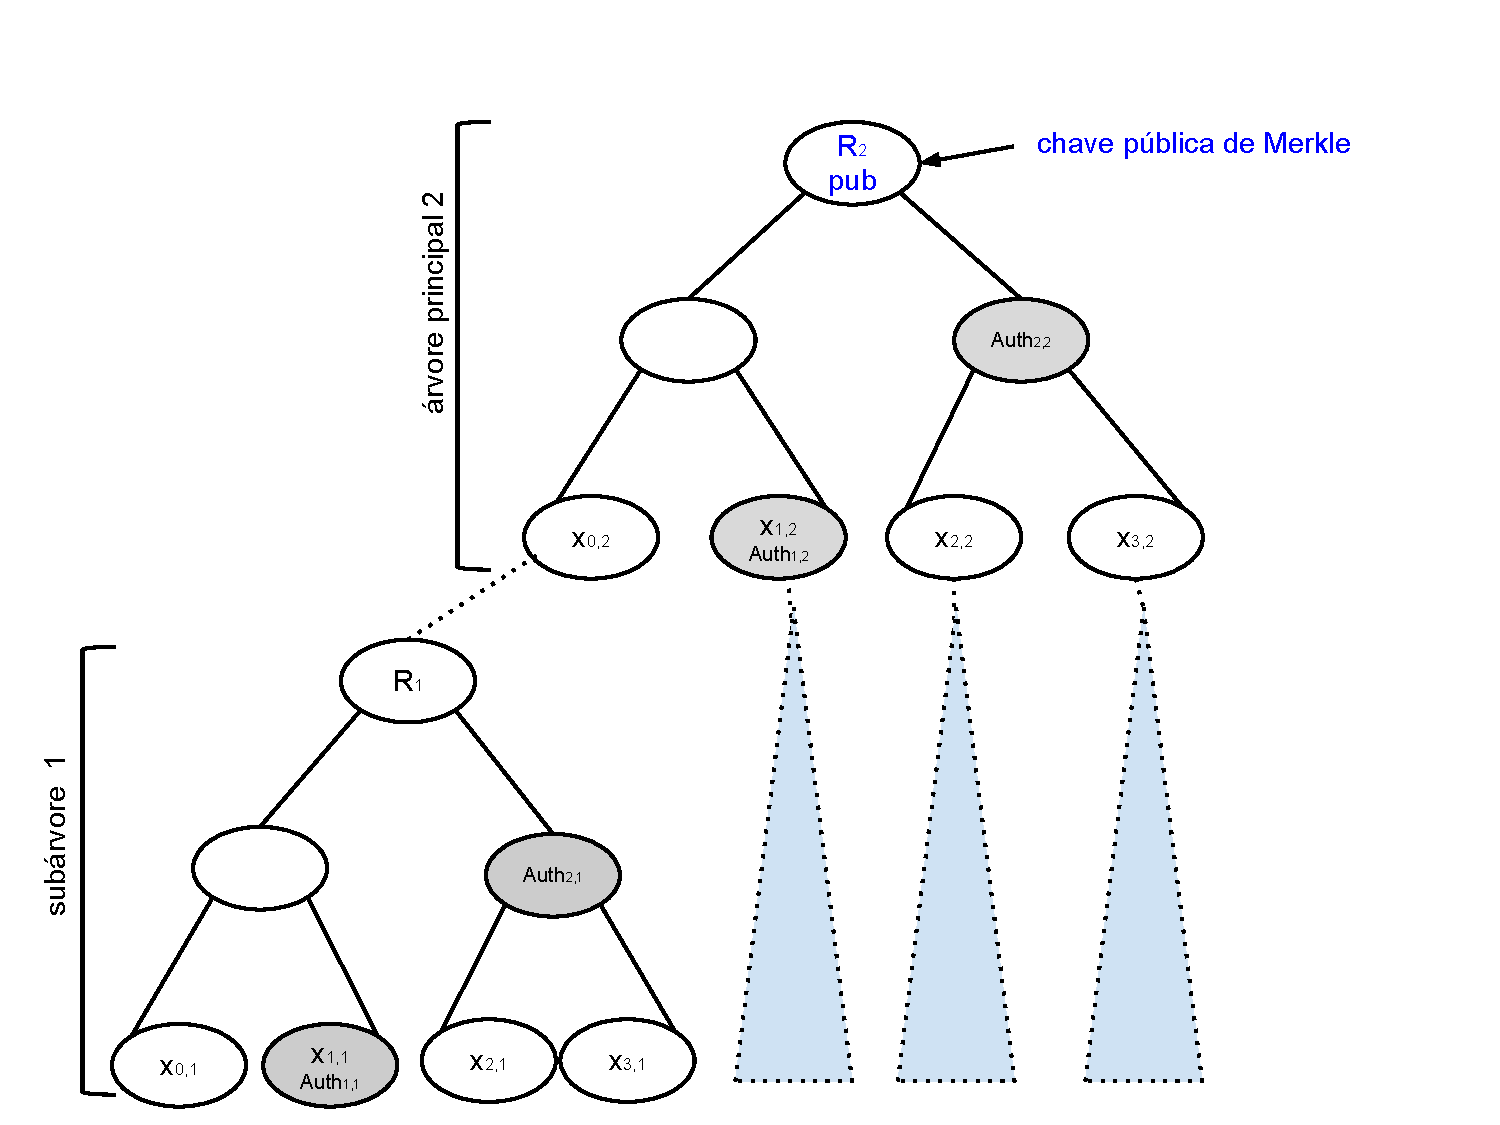
\includegraphics[scale=0.4]{figs/CMSS.pdf}
\caption{\bf Esquema de assinatura CMSS}
\label{cmss}
\end{figure}

\subsection{GMSS - Esquema de Merkle com capacidade virtualmente ilimitada de geração de assinaturas}\label{GMSS}

O esquema \textit{GMSS} foi publicado em 2007 ~\cite{buch:07}, no qual os autores propõem uma alteração no esquema de assinatura Merkle que permite assinar um número ilimitado de mensagens $2^{80}$ usando um único par de chaves. 
O esquema \textit{GMSS} foi utilizado para projetar um protocolo cliente servidor para servidores web usando \textit{SSL/TLS} que minimiza a latência e aumenta a resistência à ataques de negação de serviço.

A construção básica de \textit{GMSS} consiste de uma árvore com $T$ camadas. Subárvores em camadas diferentes podem ter alturas diferentes.
Para reduzir o custo de geração de uma assinatura, o esquema \textit{GMSS} usa a geração de uma assinatura de forma distribuída, distribuindo a geração de assinatura em cada subárvore em várias assinaturas. Este esquema também possibilita escolher parâmetros $w$ de Winternitz diferentes para subárvores em camadas diferentes, produzindo assim, assinaturas menores. 
\newline \newline \textit{Geração de chaves GMSS}: Para cada subárvore, o algoritmo de geração de chaves, \textit{W-OTS}, gera as chaves de assinatura e o Algoritmo ~\ref{arvoreHash} da Árvore de hash calcula as raízes das árvore $Raiz_{\tau ,0}$.
Os primeiros caminhos de autenticação de cada subárvore são salvos durante a geração da $Raiz$. 
Depois as assinaturas $Sig_{\tau}$ das $T$ árvores Merkle que serão usadas para a primeira assinatura são calculadas.
Como os va\-lores mudam com menos frequência para as camadas superiores, a  precomputação pode ser distribuída por várias etapas, resultando em uma melhora significativa da velocidade de assinatura e permitindo escolher grandes parâmetros $w$ de Winternitz, que resulta em assinaturas menores. 
Para garantir tamanhos pequenos de chaves privadas, foi utilizado \textit{PRNG}, onde somente a semente do \textit{PRNG} precisa ser armazenada.
\newline \newline \textit{Geração de assinatura GMSS}: A raiz de uma árvore filha é assinada com a chave de assinatura \textit{one-time} correspondente a uma certa folha de sua árvore mãe. 
$Raiz_{\tau}$ denota a raiz da árvore $\tau$.  $Sig_{\tau}$ denota a assinatura \textit{one-time} de $Raiz_{\tau}$, que é gerado usando a folha $l$ do pai de $\tau$. Os hashes da mensagem $d$ são assinados utilizando as folhas das árvores Merkle sobre a camada $T$ mais profunda. 
O número de mensagens que podem ser assinadas com um par de chaves \textit{GMSS} é $S = 2^{h_1 +...+ h_T}$, onde $h_1,...h_T$ são as alturas das subárvores. 
A assinatura \textit{GMSS} consiste do índice das folhas $s$, das assinaturas \textit{one-time} $Sig_d$ e $Sig_{\tau_{i,j_i}}$ onde $i=2,...,T$  e $j=0,...,2^{h_1+...+h_{i-1}}-1$ e dos caminhos de autenticação $Aut[\tau_{i,j_i},l_i]$ para $i=1,...,T$.

Na geração de assinatura também são calculados as raízes $Raiz_{\tau_{i,1}}$ e caminhos de autenticação $Aut[\tau_{i,1},0]$, das árvores seguintes $\tau_{i,1}$, onde $ i = 2,..., T$. 
A geração de assinatura pode ser dividida em duas partes. A primeira parte, parte \textit{online}, calcula $Sig_d$ e a assinatura. A segunda parte, parte \textit{offline}, precalcula os caminhos de autenticação e assinaturas \textit{one-time} das raízes necessárias para as próximas assinaturas. 
\newline \newline \textit{Verificação de assinatura GMSS}: O processo de verificação de \textit{GMSS} é essencialmente o mesmo que para \textit{MSS} e \textit{CMSS}. Primeiro, verifica-se a assinatura de uma só vez $Sig_d$ do hash $d$ usando o esquema \textit{one-time} de Winternitz. Então, o verificador valida as chaves públicas das raízes das subárvores e da árvore principal.

\subsection{XMSS - \textit{eXtended Merkle Signature Scheme}}
O esquema de assinatura \textit{XMSS} ~\cite{bucm:11} é uma modificação do esquema \textit{MSS}, sendo o primeiro esquema de assinatura prático comprovadamente \textit{foward secure} com exigências mínimas de segurança. %O tamanho de assinatura é reduzido para menos de $25\%$ em comparação com o melhor esquema de assinatura seguro baseado em hash.
Este esquema utiliza uma família de funções $F$ e uma família de funções de hash $G$. O esquema \textit{XMSS} é eficiente, se $G$ e $F$ são eficientes. 
Este esquema, é infalsificável sob ataques adaptativos de mensagem escolhida no modelo padrão se $G$ é resistente à segunda pré-imagem e $F$ é pseudo aleatório.
Os parâmetros de \textit{XMSS} são: o parâmetro de segurança $n \in \mathbb{N}$, o parâmetro de Winternitz $w \in \mathbb{N} (w > 1)$, 
o tamanho da mensagem em bits $m \in \mathbb{N}$, uma família de funções pseudo-aleatórias:
\[
F_n = \{f_K : \{0, 1\}^n \to \{0, 1\}^n |K \in \{0, 1\}^n \},  
\]
a altura da árvore $H \in \mathbb{N}$, uma função de hash $g_K$ escolhida aleatoriamente com distribuição uniforme da família de funções:
\[
G_n = \{g_K : \{0, 1\}^{2n} \to \{0, 1\}^n |K \in \{0, 1\}^n \}
\]
e a chave de assinatura \textit{one-time} $x \in \{0, 1\}^n$ escolhida aleatoriamente com distribuição uniforme. 

A chave de assinatura \textit{one-time} $x$ é utilizada para construir a chave de verificação \textit{one-time} $y$, através da aplicação da família de funções $F_n$. 
Neste trabalho utilizou-se a função $f_K(x)=g(Pad(K)||Pad(x))$, para uma chave $K \in \{0,1\}^n$, $x \in \{0,1\}^n$ e 
$Pad(z)=(z||10^{b-|z|-1})$ para $|z|<b$, sendo $b$ o tamanho do bloco da função de hash.

O esquema \textit{XMSS} utiliza uma versão um pouco modificada do esquema de Winternitz ~\cite{buch:11}. 
Esta modificação permite eliminar a necessidade de uma família de funções de hash resistente à colisão.
Utiliza um caminho através da família de funções em vez de uma avaliação iterada da função de hash. 
Para $K, x \in \{0, 1\}^n$, $ e \in $ $\mathbb{N}$, e $f_K \in F_n$, define-se  a função $f_{K}^{e}(x)$ como: $f_{K}^{0}(x) = K$, e para $e>0$ $f_{K}^{e}(x) = f_{K^{\prime}}(x)$, 
onde $K^{\prime} = f_{K}^{e-1}(x)$.
\newline Para o parâmetro $w$ de Winternitz, calcula-se:
$$l_1 = \Bigg \lceil \frac {m}{log_2(w)} \Bigg\rceil,\qquad  l_2=  \Bigg\lfloor \frac{log_2(l_1(w-1))}{log_2(w)}\Bigg \rfloor+1, \qquad l= l_1 + l_2. $$
A chave pública de verificação é:
$$Y=(y_1,\dots,y_l)=(f_{sk_1}^{w-1}(x),\ldots,f_{sk_l}^{w-1}(x)) .$$

O esquema \textit{W-OTS} assina mensagens binárias de comprimento $m$. Os bits da mensagem são processados na base $w$. 
A mensagem é da forma {M = ($m_1$,\dots,$m_{l_1}$)}, $m_i \in \{0,. . . , w-1\}.$ 
A soma de verificação é $c = \sum_{i=1}^{l_1} (w - 1 - m_i)$ em base de representação $w$ é anexada a $M$. 
A soma de verificação é de comprimento $l_2$. O resultado da concatenação dos blocos de $M$ com $c$ é $b=(b_1, ..., b_l)$. 
O tamanho da assinatura, das chaves de assinatura e verificação é de $l$ cadeias de $n$ bits . A assinatura é:
$$  Sig = (sig_1, ..., sig_l) = (f^{b_1}_{sk_1}(x), ..., f^{b_l}_{sk_l}(x)). $$

A árvore \textit{XMSS} é uma modificação da árvore de hash de Merkle. A árvore de altura $H$, tem $H+1$ níveis.
Utiliza função de hash $g_K$ e vetores de \textit{bitmasks} $(b_{l,j} || b_{r,j}) \in \{0,1\}^{2n}$, escolhidos aleatoriamente, 
sendo $b_{l,j}$ o \textit{bitmask} esquerdo e $b_{r,j}$ o \textit{bitmask} direito.
Os nós no nível $j$, $0 \le j \le H$, são denotados por $NO_{i,j}$, $0 \le i < 2^{H-j}$, e $0 < j \le H$.  
Os nós são calculados como: 
$$ NO_{i,j}=g_K((NO_{2i,j-1} \oplus b_{l,j})||(NO_{2i+1,j-1} \oplus b_{r,j})).$$
Os bitmasks são a principal diferença das outras árvores de Merkle, pois eles permitem substituir a resistência à colisão da família função de hash.
Podemos observar na Figura~\ref{fig:xmss} como os nós $NO_{i,j}$ da árvore do esquema \textit{XMSS} são construídos em cada nível $j$ para gerar a chave pública da árvore.

\begin{figure}[h]
\centering
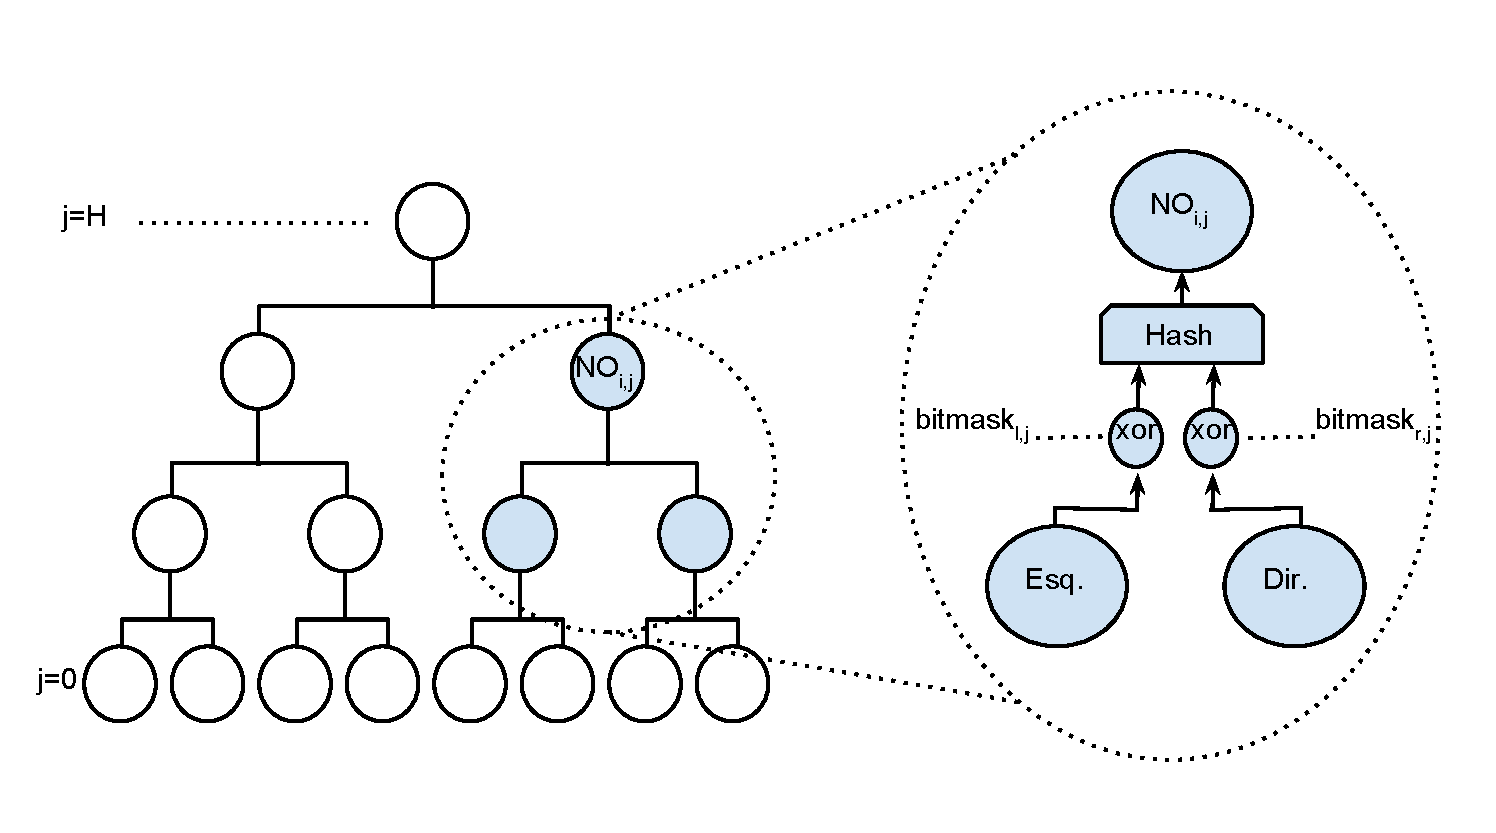
\includegraphics[width=0.6\textwidth]{figs/XMSS.pdf}
\caption{{\bf Esquema de assinatura XMSS}}.
\label{fig:xmss}
\end{figure}

\subsection{Segurança dos esquemas de assinatura baseados em funções de hash}
Nesta seção apresentamos os principais resultados conhecidos sobre a segurança dos esquemas de assinatura baseados em funções de hash.

Definimos agora o conceito de \emph{existencialmente infalsificável sob ataque adaptativo de mensagens escolhidas (existential unforgeability under adaptive chosen message attack)} de um esquema $SIGN$, onde $SIGN = (GEN, SIG, VER)$ é um esquema de assinatura e $(X, Y)$ um par de chaves gerado por $GEN$. 
Este modelo de segurança assume a existência de um poderoso falsificador. 
O falsificador tem acesso à chave pública e a um oráculo $\mathcal{O}(X, .)$ que, por sua vez, tem acesso à chave privada. 
Passa-se ao oráculo uma mensagem, e o oráculo retorna a assinatura desta mensagem. O falsificador escolhe, no máximo, $q$ mensagens  e permite que o oráculo encontre as assinaturas dessas mensagens. 
As consultas ao oráculo são adaptativas pois uma mensagem pode depender das respostas do oráculo às mensagens anteriormente consultadas. 
A saída do falsificador é um par $(M'$, $Sig')$. 
O falsificador ganha se $M$ é diferente de todas as mensagens consultadas junto ao oráculo e se $VER(M',Sig', Y) = 1$.
O esquema de assinatura SIGN é $(t, \epsilon, q)$ existencialmente infalsificável sob ataque adaptativo de mensagem escolhida se para qualquer falsificador que roda em tempo $t$, a probabilidade de sucesso para vencer o jogo acima é no máximo $\epsilon$.
Se $SIGN$ tem esta característica, é também chamado de esquema de assinatura $(t, \epsilon, q)$.
Para assinaturas \textit{one-time}, $q = 1$, pois a chave de assinatura \textit{one-time} pode ser usada apenas uma vez. 
Para o esquema de assinatura de Merkle, nós temos que $q \leqslant 2^H$.

No trabalho~\cite{bernst:09} foi provado que o esquema de assinatura one-time Lamport-Diffie é existencialmente infalsificável sob um ataque adaptativo de mensagem escolhida $(CMA seguro)$ assumindo a função \textit{one-way} é resistente à pre-imagem.
No mesmo trablho~\cite{bernst:09} foi provado que o esquema de assinatura Merkle é existencialmente infalsificável  quando a função de hash é resistente à colisão e o esquema de assinatura \textit{one-time} subjacente é existencialmente infalsificável.

Uma família de funções de hash resistente à colisão $(t_{CR}, \epsilon_{CR})$ e resistente à pré-imagem $(t_{OW}, \epsilon_{OW})$. 
O nível de segurança do \textit{MSS} é calculado conforme abaixo: 
$$\epsilon \rightarrow 2 * max\{\epsilon_{CR},2^H * 4n * \epsilon_{OW}\}$$
$$t = min\{t_{CR},t_{OW}\} - 2^H * t_{SIG} - t_{VER} - t_{GEN}$$
$$t_{GEN} \rightarrow 2^H * 6n, t_{SIG} \rightarrow 4*n(H+1), t_{VER} \rightarrow n+H$$

Nas análises efetuadas em \cite{bernst:09} para computadores clássicos, foram consideradas que as funções de hash com saída de tamanho $n$ somente admitem ataques genéricos contra suas pré imagens e resistência à colisão. 
Esses ataques são o de busca exaustiva e o ataque de aniversário. 
Quando computadores clássicos são usados, um ataque de aniversário testa $2^{n/2}$ valores hash com probabilidade de sucesso de aproximadamente $1/2$. 
Também, uma busca exaustiva de $2^n/2$ cadeias aleatórias gera uma pré-imagem de um dado valor hash com probabilidade $1/2^{n/2}$. 
Assim, nós assumimos que a família de funções de hash $\mathcal{G}$ é $(2^{n/2},1/2)$ resistente à colisão e $(2^{n/2}, 1/2^{n/2})$ resistente à préimagem.
O nível de segurança do esquema de assinatura de Merkle combinado com o esquema de assinatura one-time Lamport-Diffie é pelo menos
$$b = n/2 -1$$
se a altura da árvore Merkle é pelo menos $H\rightarrow n/3$ e o tamanho da saída da função de hash é pelo menos $n\geqslant 87$, para computadores clássicos.

\subsection{Resultados da Implementação em Software}

No trabalho\cite{ana:13} foram apresentado os resultados de uma implementação em software dos esquemas esquemas \textit{MSS}, \textit{CMSS}, \textit{GMSS} e \textit{XMSS},
utilizando uma máquina Intel Core $i7-2670$ QMCPU, $2.20$ GHz com $6$ GB de RAM.

A Tabela~\ref{tabela3} mostra os tamanhos das chaves em bytes e os tempos de execução dos algoritmos implementados com a função de hash \textit{SHA-2}. 
Definiu-se: ($C_{pub}$) tamanho da chave pública, ($C_{priv}$) tamanho da chave privada, ($C_{sig}$) tamanho da chave de assinatura, ($t_{sigOnl}$) tempo de assinatura \textit{Online}, ($t_{sigOffl}$) tempo de assinatura \textit{Offline}.
A assinatura \textit{online}, calcula a assinatura \textit{W-OTS} e a assinatura \textit{offline}, precalcula os ca\-minhos de autenticações para a próxima assinatura. 
Para o esquema \textit{GMSS} com $2$ subárvores, definimos \textit{GMSS} T=2 $(w_2,w_1)$ e para $4$ subárvores definimos \textit{GMSS T=4 $(w_4,w_3,w_2,w_1)$}, sendo
o parâmetro $w_1$ utilizado para a árvore da camada mais acima e $w_2$,$w_3$ e $w_4$ para as subárvores das camadas mais abaixo.

\begin{table}[!ht]
 \center\footnotesize
 \begin{tabular}{|p{2.0cm}|l|l|l|l|l|l|l|l|l|} \hline
   \textbf{Esquema}&\textbf{H} & \textbf{w}   & $C_{pub}$ & $C_{priv}$ & $C_{sig}$  & $t_{chaves}$ & $t_{sigOnl}$&$t_{sigOffl}$ & $t_{ver}$ \\ \hline\hline
   MSS 	    &20& 3&32 & 1316 & 3556 & 243.5 s& 0.13 ms&0.01 ms &0.11 ms\\ \hline
   MSS 	    &20& 4&32 & 1316  & 2820 & 311.5 s& 0.17 ms& 0.01 ms & 0.16 ms\\ \hline\hline
   CMSS	    &20&(3,3)& 32 & 2056 & 6472 & 0.30 s& 0.13 ms&0.25 ms &0.28 ms\\ \hline
   CMSS	    &20&(4,4)& 32 &  2056& 5000  &0.37 s& 0.17 ms& 0.32 ms &0.40 ms\\ \hline
   CMSS  &40&(3,3)& 32 & 3976  & 7112 & 269 s& 0.14 ms& 0.26 ms & 0.30 ms\\ \hline
   CMSS  &40&(4,4)& 32 & 3976  & 5640 & 384 s& 0.17 ms& 0.32 ms & 0.40 ms\\ \hline\hline
   GMSS T=2 &40&(9,3)& 32 & 3976  & 5224 & 48.1 min & 0.16 ms& 0.27 ms & 4.98 ms\\ \hline
   GMSS T=4 & 80& (3,3,3,3)&32 &9232 & 14224  &  570 s& 0.14 ms& 0.29 ms & 0.45 ms\\ \hline
   GMSS T=4 & 80& (7,7,7,3)&32 &9232 & 10864 & 50.3 min& 0.13 ms& 0.25 ms & 2.3 ms\\ \hline\hline
   XMSS	    &20&4& 1696 & 1316 &4932  & 293.6 s& 0.25 ms& 0.01 ms&0.34 ms\\ \hline

 \end{tabular}
 \caption{Tamanhos em bytes, tempos em (ms,s,min) e função SHA-2(256)}
 \label{tabela3}
\end{table}

Observamos, pela Tabela ~\ref{tabela3}, que o tamanho das chaves públicas tem $32$ bytes, exceto para o esquema \textit{XMSS} que guarda \textit{bitmasks}.
A chave privada e a assinatura são menores nos esquemas \textit{MSS} e \textit{XMSS}, pois nos outros esquemas é preciso guardar informações de $2$ ou mais árvores.

Nos gráficos da Figura~\ref{sha2sha3h20} observamos os resultado dos tempos de assinatura e verificação obtidos com $w=4$, $H=20$ utilizando as funções \textit{SHA-2} e \textit{SHA-3}.
O esquema \textit{MSS} teve os melhores tempos de assinatura e verificação, porque somente um caminho de autenticação precisa ser atualizado e checado para cada assinatura. 
Porém, o \textit{MSS} é recomendado somente para aplicações que necessitam até $2^{20}$ chaves de assinatura, tornando-se ineficiente para gerar mais chaves por consumir muitos recursos de memória.
Se forem necessárias mais chaves de assinatura, os algoritmos \textit{CMSS} e \textit{GMSS} são recomendados. 

\begin{figure}[h]
\center
\subfigure[ref1][SHA-2]{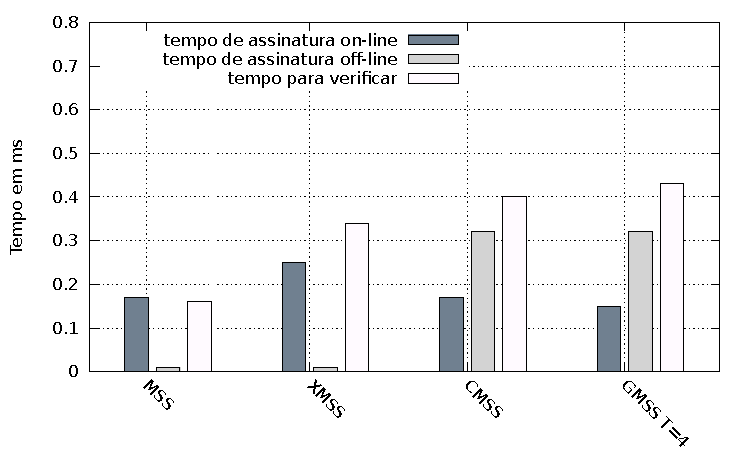
\includegraphics[width=7cm]{figs/Sha2H20w4.pdf}}
\qquad
\subfigure[ref2][SHA-3]{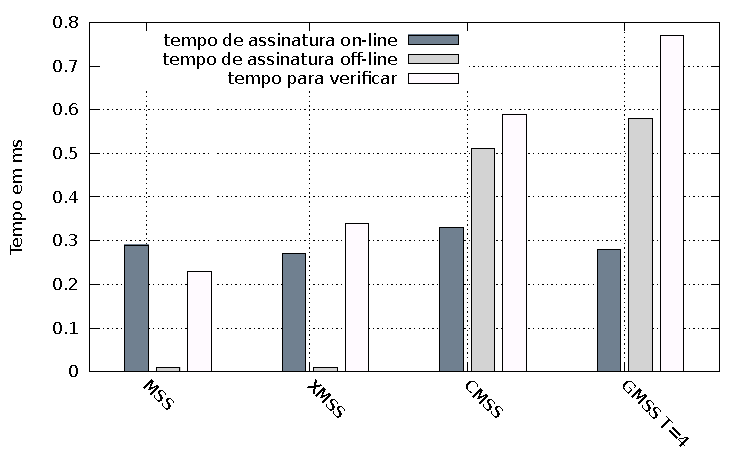
\includegraphics[width=7cm]{figs/Sha3H20w4.pdf}}
\caption{Tempos de assinatura e verificação com w=4 e H=20}
\label{sha2sha3h20}
\end{figure}


%%%%%%%%%%%%%%%%%%%%%%%%%%%%%%%%%%%%%%%%%%%%%%%%%%%%%%%%%%%%%%%%%%%%%%%%%
\section{Criptografia de chave pública baseada em sistemas multivariados}
%%%%%%%%%%%%%%%%%%%%%%%%%%%%%%%%%%%%%%%%%%%%%%%%%%%%%%%%%%%%%%%%%%%%%%%%%

Os criptossistemas multivariados de chave pública (\emph{multivariate public key cryptosystems}, ou MPKC) constituem mais uma das principais famílias de criptossistemas de chave pública considerada potencialmente resistentes até mesmo aos poderosos computadores quânticos do futuro. Esquemas MPKC têm sua segurança baseada, em última análise, na dificuldade de resolver sistemas de equações não-lineares multivariadas sobre corpos finitos. Em particular, na maior parte dos casos, tais esquemas se baseiam em resolver sistemas de equações multivariadas \textbf{quadráticas}. Esse último problema ficou conhecido como o Problema $\MQ$ (multivariate quadratic problem), e foi mostrado ser NP-difícil por Patarin~\cite{Patarin-Goubin}. MPKC tem se desenvolvido mais intensamente nas duas últimas décadas. Descobriram que algumas das construções existentes não eram tão seguras quanto se acreditava inicialmente, enquanto outras ainda permanecem viáveis.

A principal ideia em sistemas MPKC é definir uma função de mão única com alçapão que tenha como imagem um sistema não-linear de equações multivariadas sobre um corpo finito. A chave pública é dada por um conjunto de polinômios:
\[
\mathcal{P} = \{p_1(x_1,~\dots,~x_n), \cdots, p_m (x_1,~\dots,~x_n)\}
\]
onde cada $p_i$ é um polinômio não-linear (comumente quadrático) nas variáveis\\ $\textbf{x} = (x_1,~\cdots,~x_n)$:
\begin{equation} \label{eq:mq-public-polynomial}
p_k(x_1,~\dots,~x_n) := \sum_{1 \leq i \leq j \leq n}{P^{(k)}_{ij} x_i x_j} + \sum_{1 \le i \le n}{L^{(k)}_i x_i + c^{(k)}}, 0 \leq k \leq m
\end{equation}
e todos os coeficientes e variáveis estão em $\F_q$.
Para simplificar a definição anterior, usaremos notação vetorial, que é inclusive mais próxima de uma implementação:
\begin{equation} 
p_{k}(\textbf{x}) := \textbf{x} P^{(k)} \textbf{x}^{\tp} + L^{(k)} \textbf{x}^{\tp} + c^{(k)}
\end{equation}
onde $P^{(k)} \in \F^{n \times n}_{q}$ é uma matriz de tamanho $n \times n$,  formada com os coeficientes da parte quadrática de $p_k(x_1,~\dots,~x_n)$, $L^{(k)} \in \F^{n}_{q}$ é um vetor formado com os coeficientes da parte linear de $p_k(x_1,~\dots,~x_n)$, e $c^{(k)}$ denota um termo constante de $p_k(x_1,~\dots,~x_n)$. $\textbf{x}$ é o vetor linha das variáveis $[x_1,~\dots,~x_n]$.
A Figura \ref{fig:transf-quadratica} ilustra a transformação (ou mapa) puramente quadrático $\textbf{x} P^{(k)} \textbf{x}^{\tp}$ (que fornece um certo elemento no corpo finito, denotado por $h_k \in \F_q$) em termos de matrizes e vetores.

\begin{figure}[htbp] \centering
    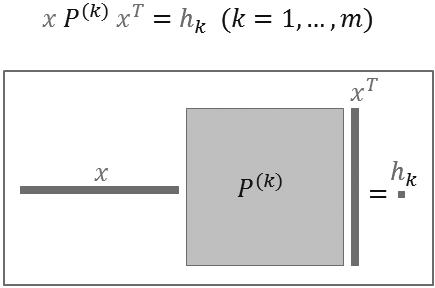
\includegraphics[scale=0.7]{figs/transformacao-quadratica.png}
\caption{Mapa ou Transformação Puramente Quadrática}
\label{fig:transf-quadratica}
\end{figure}

%$P : \mathbb{F}^n \rightarrow \mathbb{F}^m$ difícil de se resolver e introduzindo-se um alçapão secreto que torna o sistema solúvel em tempo hábil. O sistema público pode ser representa por um conjunto de $m$ polinômios em $n$ variáveis conforme mostrado a seguir

A seguir é dada uma definição mais formal para o Problema $\MQ$.

\begin{definition}[\textbf{Problema $\MQ$}] Resolva o sistema $p_1(\textbf{x})=p_2(\textbf{x})=\cdots=p_m(\textbf{x})=0$, onde cada $p_i$ é quadrático em $\textbf{x} = (x_1,~\dots,~x_n)$. Todos os coeficientes e variáveis estão em $K = \F_q$, o corpo de $q$ elementos.
\end{definition}

Em outras palavras, o objetivo do  problema $\MQ$ é encontrar uma solução $x$ para um dado mapa $\mathcal{P}$. Garey e Johnson provaram em 1979 \cite[página 251]{garey-johnson} que a variante decisional do problema $\MQ$ é um problema NP-completo sobre corpos finitos. Mas infelizmente, aplicando-se equivalência polinomial de problemas de busca e decisão para linguagens NP-completas \cite{bellare-goldwasser}, o resultado de Garey e Johnson fornece apenas uma dificuldade de pior caso do problema $\MQ$ decisional. E, de fato, a complexidade do problema $\MQ$ depende fortemente da relação entre $n$ e $m$, além da estrutura dos polinômios.

Curiosamente, foi mostrado que o problema $\MQ$ se torna solúvel em \emph{tempo polinomial} usando a técnica de \emph{linearização} para sistemas subdeterminados em corpos de característica par quando $n \ge m(m+1)$ e, em corpos de característica ímpar quando $n \ge 2^{m/7}(m+1)$  \cite[Sec. 7]{kipnis-patarin-goubin-ext} \cite{courtois-goubin-meier-tacier}, ou para sistemas sobredeterminados com $m \ge n(n+1)/2$, ou ainda melhor, $m \ge n(n-1)/2$ para o caso especial $\F_2$. %fonte: tese do Enrico

Por outro lado, todos os esquemas de assinatura $\MQ$ propostos até o momento não têm sua segurança baseada somente no problema $\MQ$. Para reconstruir a chave privada, ou ainda encontrar uma equivalente, é necessário resolver um problema relacionado, o Problema do Isomorfismo de Polinômios ou $IP$, proposto por Patarin \cite{patarin-ip}. Note que para todos os polinômios de algum grau fixado, todos os argumentos seguintes são polinômios redutíveis a polinômios de grau 2. %Ademais, nos restringimos  a problemas de \emph{busca} e não de \emph{decisão}. Bellare e Goldwasser demonstraram em \cite{bellare-goldwasser} que para linguagens NP-completas, problemas de busca e decisão são polinomialmente equivalentes, mas isso não é necessariamente verdadeiro para todos os problemas em NP. Como exemplo, temos o problema da fatoração inteira, onde é possível decidir em tempo polinomial se um número é composto, mas até hoje não se sabe como se encontrar seus fatores primos em tempo também polinomial.


\begin{definition}[\textbf{Problema do Isomorfismo de Polinômios ($IP$)}] \label{def:IP}
Sejam $m,n \in \N$ fixados e arbitrários. Sejam também $\mathcal{P},\mathcal{Q} : \F_q^n \rightarrow \F_q^m$ dois mapas quadráticos e $\mathcal{T} \in \F_q^{mxm}$, $\mathcal{S} \in \F_q^{nxn}$ transformações lineares bijetoras, tais que $\mathcal{P} = \mathcal{T} \circ \mathcal{Q} \circ \mathcal{S}$. Sabendo-se $\mathcal{P}$ e $\mathcal{Q}$, encontre $\mathcal{T}$ e $\mathcal{S}$.
\end{definition}

Em outras palavras, o objetivo do problema $IP$ é encontrar $\mathcal{T}$ e $\mathcal{S}$ para um dado par $(\mathcal{P},\mathcal{Q})$. Note que, originalmente, $\mathcal{S}$ foi definida como uma transformação afim em vez de linear \cite{patarin-goubin-courtois}. Mas,  Braeken \emph{et al.} \cite[Sec. 3.1]{braeken-wolf-preneel} perceberam que a parte constante não é importante para a segurança de certos esquemas $\MQ$ e, portanto, pode ser omitida.

\subsection{Construção de Chaves $\MQ$}

De forma genérica, a chave privada é composta das transformações lineares $\mathcal{T}$ e $\mathcal{S}$ mais a transformação quadrática $\mathcal{Q}$. Note que a transformação $\mathcal{Q}$ possui certa estrutura especial com alçapão (sendo duas estruturas distintas de $\mathcal{Q}$ descritas na Seção~\ref{sec:assinaturas-uov-rainbow} para as assinaturas UOV e Rainbow), que permitirá ao signatário resolver facilmente o sistema $\MQ$ público para gerar assinaturas válidas. A chave pública será dada pela composição $\mathcal{P} = \mathcal{T} \circ \mathcal{Q} \circ \mathcal{S}$. Em alguns esquemas de assinatura não é necessário utilizar transformação $\mathcal{T}$, pois ela se reduz à identidade~\cite[Capítulo~6]{bernstein-buchmann-dahmen}.

A principal diferença entre esquemas de assinatura $\MQ$ distintos está na estrutura de alçapão de $\mathcal{Q}$. Como a chave pública tem a mesma forma na maioria desses esquemas, o procedimento de verificação de uma assinatura é o mesmo, ou seja, testar se uma dada assinatura $\textbf{x}$ é solução de um sistema quadrático público $p_k(\textbf{x})=h_k(m)$. Para consultar as várias construções distintas do mapa privado $\MQ$ veja \cite{wolf-preneel-taxonomy}.

Vale mencionar aqui uma otimização óbvia nas matrizes públicas $P^{(k)}$, que proporciona aproximadamente um fator dois de redução. Observando-se a definição do somatório da parte quadrática do polinômio $p_k(x_1,~\dots,~x_n)$ (Equação \ref{eq:mq-public-polynomial}), nota-se que o coeficiente do termo $x_i x_j$ é $P^{(k)}_{ij} + P^{(k)}_{ji}$, ou seja, pode-se atualizar o coeficiente $P^{(k)}_{ij}$ da matriz com o valor $P^{(k)}_{ij} + P^{(k)}_{ji}$ e o coeficiente $P^{(k)}_{ji}$ com zero para $i \leq j \leq n$, o que torna cada matriz $P^{(k)}$ triangular superior. Após essa otimização, podemos definir uma única matriz pública que será útil em algumas construções $MQ$. Trata-se da \emph{matriz pública de coeficientes}, denotada $M_{P}$, e é formada linearizando-se os coeficientes de cada uma das $m$ matrizes $P^{(k)}$ já na forma triangular superior. A Figura \ref{fig:matriz-publica-coefs}, ilustra essa construção.

\begin{figure}[htbp] \centering
    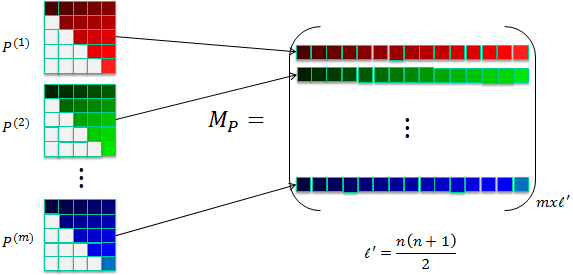
\includegraphics[scale=0.9]{figs/matriz-publica-coefs.png}
\caption{Matriz Pública de Coeficientes}
\label{fig:matriz-publica-coefs}
\end{figure}


\subsection{Assinaturas UOV e Rainbow} \label{sec:assinaturas-uov-rainbow}

Uma das principais famílias de assinaturas $\MQ$ é a construção \emph{Unbalanced Oil and Vinegar}, ou UOV proposto por Patarin~\cite{kipnis-patarin-goubin}. O nome UOV provém do fato de as variáveis estarem particionadas em duas classes, chamadas de \emph{vinagres} e \emph{azeites}, de tal maneira que variáveis da classe azeite não ocorrem juntas em nenhum termo quadrático. Essa estrutura constitui o alçapão, que permite reduzir o sistema quadrático completo a um sistema linear nos azeites, desde que os vinagres sejam conhecidos (ou escolhidos ao acaso), para simplificar os termos onde ocorrem. O alçapão é protegido pela dificuldade conjecturada do problema IP.

Formalmente, o alçapão consiste de um mapa puramente quadrático, denominado mapa central, $Q : \F^n \rightarrow \F^m$ com 
\[
Q = \{f_1(u_1,~\dots,~u_n), \dots, f_m (u_1,~\dots,~u_{n})\}
\]
e
\begin{equation} 
f_{k}(u_1, \dots, u_{n}) := \sum_{1 \leq i \leq j \leq n}{Q^{(k)}_{ij} u_i u_j} \equiv  u Q^{(k)} u^{\tp}
\end{equation}

O mapa central tem uma restrição adicional em seus polinômios $f_{k}(u_1, \dots, u_{n})$. Impõe-se que certa parte de seus coeficientes sejam nulos. O conjunto de variáveis $u$ é dividido em dois subconjuntos, o das variáveis vinagre $u_i$ com $i \in V = \{1, \cdots, v \}$ e o das variáveis azeite $u_i$ com $i \in O = \{v+1, \cdots, n\}$ que contém $m=n - v$ elementos. A restrição é que os polinômios $f^{(k)}$ não contenham nenhum termo cruzando duas variáveis azeite. Isso evita que apareçam termos quadráticos e/ou cruzados nos azeites. Dessa forma, restam apenas termos misturando os seguintes tipos de variáveis $v \times v$ e $o \times v$. Patarin mostrou que, com essa construção, podemos chutar  valores arbitrários para os vinagres, resultando em um sistema linear nas variáveis azeite. Esse sistema tem alta probabilidade de apresentar uma solução, i.e. $1-1/q$, e pode ser resolvido por eliminação gaussiana com complexidade $\bigO{n^3}$. A estrutura dos polinômios privados é a seguinte:

\begin{equation} \label{eq:mq-polynomial-q}
f^{(k)}(u_1,\cdots,u_n) := \sum_{i, j \in V, \; i \le j}^{} Q_{ij}^{(k)} u_i u_j + \sum_{i \in V, \; j \in O}^{} Q_{ij}^{(k)} u_i u_j
\end{equation}

Para gerar uma assinatura $x \in \F_q^n$ de uma dada mensagem, particularmente de seu hash criptográfico $h \in \F_{q}^m$, o signatário deve inverter a transformação $P(x) = Q(S(x)) = h$. Definindo $x' = xS$, resolve-se primeiro o sistema multivariado, $x' Q^{(k)} x'^\tp = h_k$, $1 \le k \le m$, para encontrar $x'$. Por fim, recupera-se a assinatura $x = x' S^{-1}$.

Conforme explicado anteriormente, a estrutura das matrizes $Q^{(k)}$  permite que o sistema $\MQ$ seja resolvido de forma eficiente, escolhendo $v$ variáveis $vinagre$ ao acaso e resolvendo o sistema linear resultante para encontrar as $m$ variáveis $azeite$ em função dos vinagres escolhidos. Caso o sistema linear não tenha solução, repete-se o processo escolhendo-se novas variáveis vinagre.

Uma assinatura $x$ de $h$ é válida, se e somente, se todos os polinômios $p^{(k)}$ da chave pública forem satisfeitos, i.e. $p^{(k)}(x_1,\cdots,x_n) = P^{(k)}(x) = xP^{(k)}x^T = h_k$, $1 \le k \le m$. A consistência da verificação $P(x)\overset{?}{=}h$ é mostrada a seguir
\begin{align*}
 P(x) &= x P x^T \\
                   &= x (Q \circ S) x^\tp \\ 
                   &= x (SQS^T) x^T \\
                   &= (x'S^{-1}) (SQS^\tp) (x'S^{-1})^\tp \\
                   &= x'(S^{-1} S)Q (S^\tp (S^{-1})^T) x'^\tp \\
                   &= x' I Q I x'^\tp \\
                   &= x' Q x'^\tp \\
                   &= h. \\
\end{align*}

Historicamente, o esquema UOV deriva da construção \emph{Oil and Vinegar}, ou \\OV~\cite{Patarin}, onde o número de vinagres e o número de azeites é o mesmo (balanceado), mas que se mostrou inseguro \cite{kipnis-shamir}. Em seguida, notou-se que é possível torna-lo seguro, adotando-se quantidades desbalanceadas de azeites e vinagres $v > m$, o que originou o esquema de assinatura UOV (Unbalanced Oil and Vinegar) \cite{kipnis-patarin-goubin}. A Figura \ref{fig:uov-trapdoor} ilustra a estrutura vetorial de cada polinômio privado UOV

\begin{figure}[htbp] \centering
    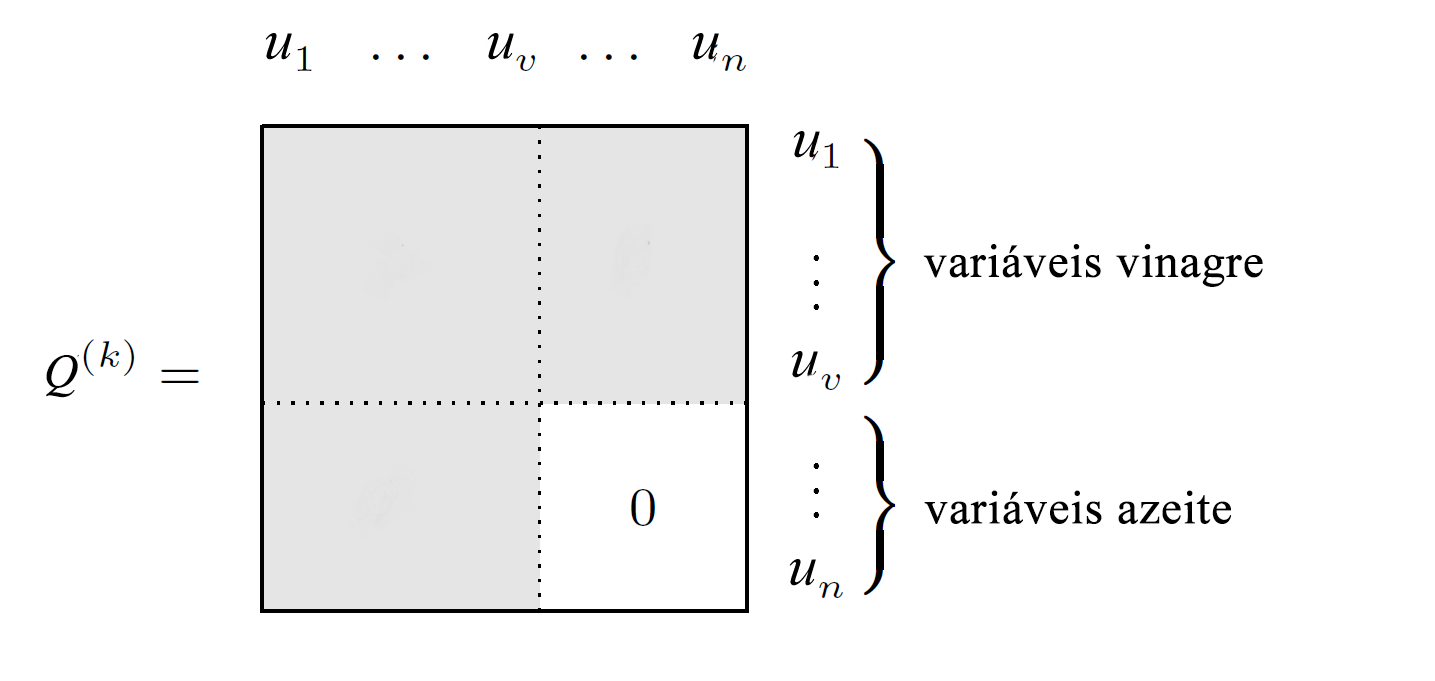
\includegraphics[scale=0.25]{figs/uov-trapdoor.png}
\caption{Mapa Central UOV}
\label{fig:uov-trapdoor}
\end{figure}

Para camuflar a estrutura dos polinômios $f^{(k)}$, é aplicada uma transformação linear inversível $\mathcal{S} \in \F^{nxn}_q$ à direita de $\mathcal{Q}$. O mapa público resultante é $\mathcal{P} = \mathcal{Q}  \circ \mathcal{S}$. A chave privada é dada pelo par $sk := (\mathcal{Q},\mathcal{S})$ e a chave pública é composta pelos polinômios $pk := P(x_1,\cdots,x_n) = \{p^{(1)}(x_1,\cdots,x_n),\cdots,p^{(m)}(x_1,\cdots,x_n)\}$.

Assim, fica claro que a segurança do sistema não é baseada somente no problema $\MQ$ e, de fato, recuperar a chave privada recai na dificuldade de decompor $\mathcal{P}$ em $\mathcal{Q}$ e $\mathcal{S}$, ou seja, resolver o problema $IP$.

Uma variante do UOV é a família de assinaturas Rainbow~\cite{ding-schmidt}  proposta por Ding e Schmidt, e tem como principal vantagem a obtenção de assinaturas mais curtas que as encontradas em UOV simples \cite[Seção~3]{thomae}.

O Rainbow tem como ideia básica a separação das $m$ equações em bandas e o particionamento das variáveis de acordo, ou seja, cada banda tem seus próprios \emph{vinagres} e \emph{azeites}, todas as variáveis de uma banda tornam-se os vinagres da banda seguinte, e os azeites de cada banda são calculados em funçãos dos vinagres da mesma.

Em geral o mapa central é dividido em duas bandas, pois essa configuração se mostrou a mais apropriada, no sentido de evitar certos ataques estruturais e ainda assim manter as assinaturas curtas~\cite{thomae}.

\begin{figure}[htbp]
	\centering
		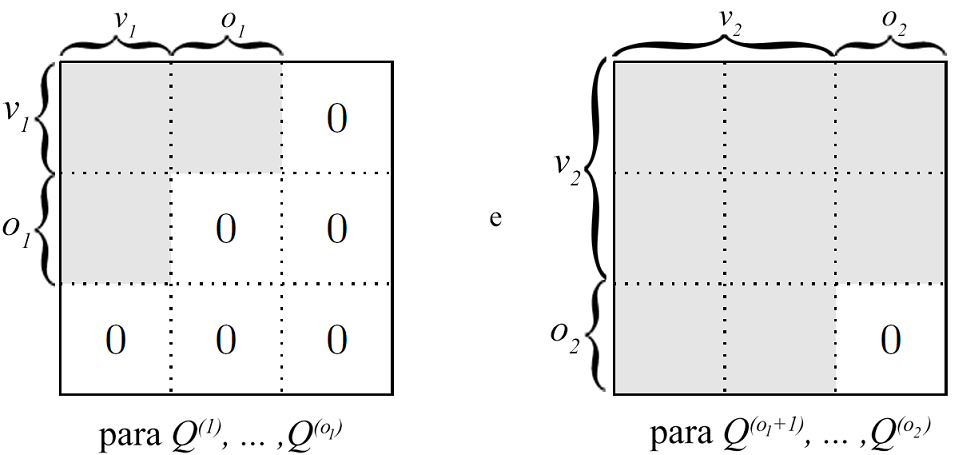
\includegraphics[width=0.7\textwidth]{figs/mapa_central_Rainbow.png}
	\caption{mapa central $Q$ do esquema Rainbow de duas bandas}
	\label{fig:trapdoorRainbow}
\end{figure}

O mapa central $Q$ dessa configuração do Rainbow é dividido em duas camadas caracterizadas pela estrutuda de suas matrizes como na Figura \ref{fig:trapdoorRainbow} onde $v_1$ e $o_1$ são o número de vinagres e azeites da primeira camada e $v_2$ e $o_2$ são o número de vinagres e azeites da segunda camada, lembrando que $v_2$ é igual ao número de vinagres e azeites da camada anterior.


O processo de assinatura é semalhante ao UOV, escolhendo ao acaso os \emph{vinagres} da primeira banda para calcular seus \emph{azeites}, da mesma maneira que é feito no UOV, e em seguida usando todas essas variáveis como \emph{vinagres} da próxima banda.

\subsection{Assinatura Cyclic UOV}
Um passo interessante na direção de redução de chaves UOV/Rainbow foi dado através das construções Cyclic UOV/Rainbow \cite{petzoldt-bulygin-buchmann:cyclicouv,petzoldt-bulygin-buchmann:cyclicrainbow}. Analisando a estrutura das chaves UOV, os autores notaram a existência de uma relação linear entre parte do mapa quadrático público e do mapa quadrático privado. Essa relação pôde ser explorada para gerar pares de chave de forma diferente do usual e reduzir assim o tamanho da chave pública. A ideia foi primeiro calcular a parte quadrática da chave pública com uma estrutura compacta desejada e a partir daí calcular a parte quadrática da chave privada utilizando-se a relação linear encontrada. 

Portanto, é possível obter chaves públicas mais compactas enquanto as chaves privadas permanecem com aparência aleatória e sem estrutura. A estrutura sugerida por Petzoldt \emph{et. al.} foi a de matrizes circulantes, daí o nome Cyclic UOV \cite{petzoldt-bulygin-buchmann:cyclicouv}. Matrizes circulantes são bastante compactas, uma vez que podem ser representadas simplesmente por sua primeira linha. Logo, a chave pública pode ser armazenada de forma mais eficiente, além de possibilitar algumas vantagens em processamento, como técnicas de Karatsuba e Fast Fourier Transform (FFT).

A construção das chaves Cyclic UOV pode ser descrita da seguinte maneira. Primeiramente, gera-se uma transformação linear $S \in F^{n \times n}_q$ inversível, onde $S_{ij} \Samples \F_q, 1 \leq i,j \leq n$ e, a partir de $S$,  calcula-se a relação linear proposta por \emph{Petzoldt et. al.}, denotada por $A_{UOV} := \alpha^{rs}_{ij}$:

\[ \alpha^{rs}_{ij} = \left\{ 
   \begin{array}{l l}
    S_{ri} \cdot S_{si} \textrm{, i=j}\\
    S_{ri} \cdot S_{sj} + S_{rj} \cdot S_{si} \textrm{, caso contrário}
   \end{array} \right.\]

Para ilustrar como as matrizes pública e privada de coeficientes, $M_{P}$ e $M_{F}$, se relacionam, temos inicialmente as Figuras \ref{fig:matriz-publica-coefs-2} e \ref{fig:matriz-privada-coefs-2} que separam as partes de interesse dessas matrizes.

\begin{figure}[htbp] \centering
    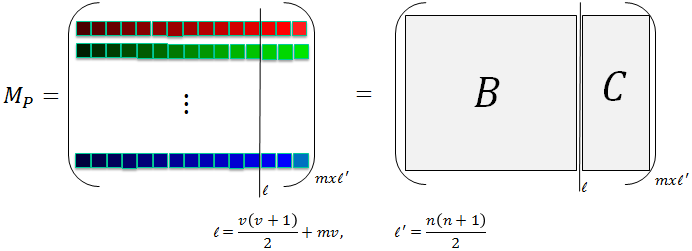
\includegraphics[scale=0.8]{figs/matriz-publica-coefs-2.png}
\caption{Cyclic UOV -- Matriz Pública de Coeficientes}
\label{fig:matriz-publica-coefs-2}
\end{figure}

\begin{figure}[htbp] \centering
    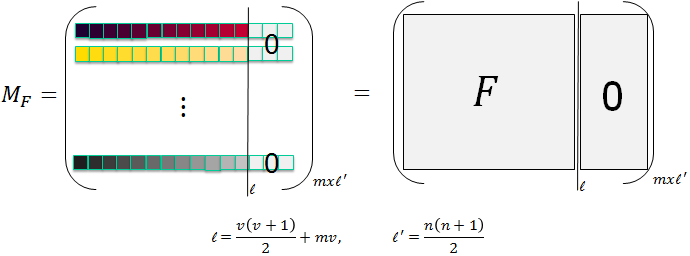
\includegraphics[scale=0.8]{figs/matriz-privada-coefs-2.png}
\caption{Cyclic UOV -- Matriz Privada de Coeficientes}
\label{fig:matriz-privada-coefs-2}
\end{figure}

Os blocos $B$ de $M_{P}$ e $F$ de $M_{F}$ se relacionam através da seguinte expressão $B := F \cdot A_{UOV}(S)$. Dessa forma, na geração de chaves, pode-se primeiro gerar a matriz $M_{P}$ com $B$ sendo uma matriz circulante e calculando-se, posteriormente, $F := B \cdot A^{-1}_{UOV}(S)$. Essa construção foi capaz de reduzir a chave pública UOV em cerca de 6 vezes para o nível de segurança de 80 bits.

Como mencionado anteriormente, assinaturas $\MQ$ têm se desenvolvido mais intensamente nas duas últimas décadas, reunindo várias propostas em direção à redução do tamanho das chaves que é sua principal desvantagem. A Tabela \ref{tab:comparacao-mq-circulante} ilustra algumas propostas.

\begin{table}\centering
\caption{Evolução das assinaturas $\MQ$}\label{tab:comparacao-mq-circulante}
\footnotesize
\begin{tabular}{lcccccc}\hline
proposta                              & $|sk|$        & $|pk|$      & $|hash|$  & $|sig|$ & ref.\\
\hline
Rainbow($\F_{2^4}$, 30, 29, 29)      & \,75.8 KiB & 113.4 KiB & 232    & 352 & \tiny \cite{petzoldt-bulygin-buchmann:params}\\ 
Rainbow($\F_{31}$, 25, 24, 24)        & \,59.0 KiB & 77.7 KiB & 232       & 392 & \tiny \cite{petzoldt-bulygin-buchmann:params}\\ 
CyclicUOV($\F_{2^8}$, 26, 52)         & \,14.5 KiB & 76.1 KiB & 208       & 624 &\tiny \cite{petzoldt-bulygin-buchmann:cyclicrainbow}\\
NC-Rainbow($\F_{2^8}$, 17, 13, 13)    & \,25.5 KiB & 66.7 KiB & 384  & 672 & \tiny \cite{yasuda-sakurai-takagi}\\
Rainbow($\F_{2^8}$, 29, 20, 20)       & \,42.0 KiB & 58.2 KiB & 272    & 456  & \tiny \cite{petzoldt-bulygin-buchmann:params}\\ 
CyclicLRS($\F_{2^8}$, 26, 52)         & \,71.3 KiB & 13.6 KiB & 208       & 624  & \tiny \cite{petzoldt-bulygin-buchmann:LRS}\\
UOVLRS($\F_{2^8}$, 26, 52, 26)        & \,71.3 KiB & 11.0 KiB & 208   & 624   & \tiny \cite{petzoldt-bulygin-buchmann:LRS}\\
CyclicRainbow($\F_{2^8}$, 17, 13, 13) & \,19.1 KiB & 10.2 KiB & 208 & 344  & \tiny \cite{petzoldt-bulygin-buchmann:cyclicrainbow}\\
\hline
\end{tabular}
\end{table}


%%%%%%%%%%%%%%%%%%%%%%%%%%%%%%%%%%%%%%%%%%%%%%%%%%%%%%%%%%%%%%%%%
\section{Criptografia baseada em códigos corretores de erros}\label{sec:errorcodes}
%%%%%%%%%%%%%%%%%%%%%%%%%%%%%%%%%%%%%%%%%%%%%%%%%%%%%%%%%%%%%%%%%

Nesse capítulo falaremos sobre a teoria e a prática de sistemas criptográficos baseados em códigos corretores de erros.

A teoria da codificação tem como objetivo assegurar que, ao transmitir uma \\coleção de dados através de um canal sujeito a ruídos (ou seja, a perturbações nos dados enviados), o destinatário dessa transação possa recuperar a mensagem original. Para isso, devem-se encontrar maneiras eficientes de adicionar informação redundante à mensagem original de tal forma que, caso a mensagem chegue ao destinatário contendo erros (existindo inversão em certos bits, para o caso de mensagens binárias), o recebedor possa corrigi-la. A Figura\ref{fig:canalcomunicacao}, baseada em~\cite{huffman-pless}, ilustra bem esta situacão:

\begin{figure}[htbp]
    \centering
		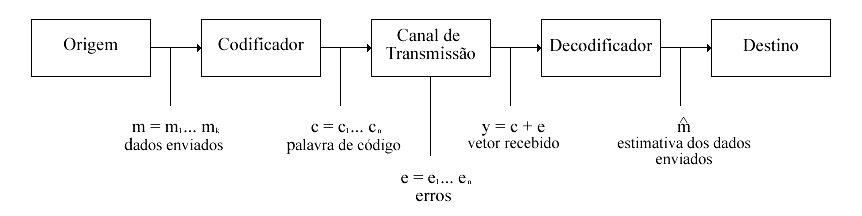
\includegraphics[width=1.0\textwidth]{figs/canalcomunicacao.png}
	\caption{Canal de Comunicação}
	\label{fig:canalcomunicacao}
\end{figure}

No contexto criptográfico, a primitiva consiste em adicionar erros em uma palavra de um código corretor de erros e calcular uma síndrome relativa a matriz de verificação de paridade desse código.

O primeiro desses sistemas foi um esquema de encriptação de chave pública proposto por Robert J. McEliece em 1978~\cite{McEliece}. A chave privada é um código de Goppa (que será revisado na seção~\ref{subsubsec:goppa}) aleatório, binário e irredutível, e a chave pública é uma matriz geradora aleatória com uma versão permutada desse código. O texto encriptado é uma palavra de código no qual alguns erros foram introduzidos, e somente o dono da chave privada pode remover esses erros (e, consequentemente, decriptar a mensagem). Alguns anos mais tarde alguns ajustes de parâmetros foram necessários para manter o nível de segurança, mas não é conhecido, até hoje, nenhum ataque que possa quebrar esse criptossistema.


\subsection{Códigos lineares}\label{subsec:linearcodes}

Para um melhor entendimento técnico desse capítulo, primeiramente vamos explicar algumas noções fundamentais utilizadas no âmbito da criptografia baseada em códigos.

No contexto que segue, todos os índices de matrizes e vetores são numerados a partir de zero, a menos que explicitamente indicado de outra forma. Seja $p$ um primo, e seja $q = p^m$ para algum inteiro $m > 0$. $\F_q$ denota o corpo finito com $q$ elementos. O grau de um polinômio $g \in \F_q[x]$ denota-se $\deg(g)$. Define-se também a noção de \emph{peso de Hamming} e \emph{distância de Hamming}:

\begin{definition}\label{def:hamming}
O \emph{peso de Hamming} de um vetor $u \in \mathcal{C} \subseteq \F_q^n$ é o número de coordenadas não nulas de $u$, i.e. $\wt(u) = \#\{i, \; 0 \leqslant i < n \mid u_i \neq 0\}$. A \emph{distância de Hamming} entre dois vetores $u, v \in \mathcal{C} \subseteq \F_q^n$ é o número $\dist(u, v)$ de coordenadas em que esses vetores diferem, i.e. $\dist(u, v) := \wt(u - v)$.
\end{definition}


Agora vamos introduzir alguns conceitos úteis à tarefa de codificar mensagens. O
primeiro deles se refere a \emph{código linear}, que pode ser definido como:

\begin{definition}\label{def:code}
Um código linear $[n,k]$ (de comprimento $n$ e dimensão $k$) sobre o corpo $\F_q$ é um subespaço vetorial $\mathcal{C}$ de dimensão $k$ do espaço $\F_q^n$.
\end{definition}
Um vetor qualquer $u \in \mathcal{C}$ é também chamado palavra de código (ou, abreviadamente, uma palavra) de $\mathcal{C}$.

Sendo um espaço vetorial, $\mathcal{C}$ é representado por uma base, que pode ser escrita na forma de uma \emph{matriz geradora}:

\begin{itemize}
    \item Uma matriz geradora $G$ de $\mathcal{C}$ é uma matriz sobre $\F_q$ tal que $\mathcal{C} = \left\langle G \right\rangle$, onde $\left\langle G \right\rangle$  indica o espaço vectorial gerado pelas linhas de $G$. Normalmente as linhas de $G$ são independentes e a matriz possui dimensão $k \times n$. De outra forma: $\exists G \in \F_q^{k \times n} : \mathcal{C} = \{ u G \in \F_q^n \mid u \in \F_q^k \}$.
    \item Dizemos que uma matriz geradora $G$ está na forma sistemática se suas primeiras $k$ colunas formam a matriz identidade.
    \item O chamado \emph{código dual} $\mathcal{C}^\bot$ é o código ortogonal de $\mathcal{C}$ para o produto escalar sobre $\F_q$ e é um código linear de dimensão $n \times (n - k)$ sobre $\F_q$.
\end{itemize}

Alternativamente, $\mathcal{C}$ é inteiramente caracterizado como o núcleo de uma transformação linear especificada por uma \emph{matriz de verificação de paridade} (ou abreviadamente \emph{matriz de paridade}): 

\begin{itemize}
    \item Uma matriz de paridade $H$ sobre $\mathcal{C}$ é uma matriz geradora de $\mathcal{C}^\bot$. De outra forma: $\exists H \in \F_q^{r \times n} : \mathcal{C} = \{ v \in \F_q^n \mid H v^{\tp} = 0^r \in \F_q^r \}$, onde $r = n - k$ é a codimensão de $\mathcal{C}$ (ou seja, a dimensão do espaço ortogonal $\mathcal{C}^\bot$).
\end{itemize}

Torna-se fácil ver que $G$ e $H$, embora não sejam unicamente definidas (pois não há uma única base para $\mathcal{C}$ nem para $\mathcal{C}^\bot$), relacionam-se por $H G^{\tp} = O \in \F_q^{r \times k}$.

A transformação linear definida por uma matriz de paridade é chamada \emph{função síndrome} do código. O valor dessa transformação sobre um vetor qualquer $u \in \F_q^n$ denomina-se \emph{síndrome} desse vetor. Claramente, a síndrome de qualquer palavra de código é sempre nula.


\begin{definition}\label{def:codedist}
A \emph{distância} (ou \emph{distância mínima}) de um código $\mathcal{C} \subseteq \F_q^n$ é a distância de Hamming mínima entre palavras de $\mathcal{C}$, i.e. $\dist(\mathcal{C}) = \min\{\wt(u) \mid u \in \mathcal{C}\}$.
\end{definition}
Escreve-se $[n,k,d]$ para um código $[n,k]$ cuja distância mínima é (pelo menos) $d$. Se $d \geqslant 2t + 1$, diz-se que o código é capaz de corrigir pelo menos $t$ erros, no sentido de existir não mais que uma única palavra de código a uma distância de Hamming não superior a $t$ de qualquer vetor de $\F_q^n$.

Vários problemas computacionais envolvendo códigos são intratáveis, começando com a própria determinação da distância mínima. Os seguintes problemas têm importância para criptografia baseada em códigos:

\begin{definition}[Decodificação geral]\label{def:gdp}
Seja $\F_q$ um corpo finito, e seja $(G, w, c)$ uma tripla consistindo de uma matriz $G \in \F_q^{k \times n}$, um inteiro $w < n$, e um vetor $c \in \F_q^{n}$. O \emph{problema da decodificação geral (GDP)} consiste em determinar se existe um vetor $m \in \F_q^{k}$ tal que $e = c - mG$ tenha peso de Hamming $\wt(e) \leqslant w$.
\end{definition}
O problema de busca associado ao GDP consiste em calcular o vetor $m$ dada a palavra com erros $c$.

\begin{definition}[Decodificação de síndromes]\label{def:sdp}
Seja $\F_q$ um corpo finito, e seja $(H, w, s)$ uma tripla consistindo de uma matriz $H \in \F_q^{r \times n}$, um inteiro $w < n$, e um vetor $s \in \F_q^{r}$. O \emph{problema da decodificação de síndrome (SDP)} consiste em determinar se existe um vetor $e \in \F_q^{n}$ com peso de Hamming $\wt(e) \leqslant w$ tal que $H e^{\tp} = s^{\tp}$.
\end{definition}
O problema de busca associado ao SDP consiste em calcular o padrão de erro $e$ dada sua síndrome $s_e := e H^{\tp}$.

Tanto o problema da decodificação geral quanto o problema da decodificação de síndromes para códigos lineares são $NP$-completos~\cite{berlekamp-mceliece-vantilborg}.

Em contraste com os resultados gerais, o conhecimento da estrutura de certos códigos torna o GDP e o SDP solúveis em tempo polinomial.
Uma estratégia básica para definir criptossistemas baseados em códigos é, portanto, manter secreta a informação sobre a estrutura do código, e publicar um código relacionado sem estrutura aparente (portanto, por hipótese difícil de decodificar).

\subsubsection{Códigos de Goppa}\label{subsubsec:goppa}

Uma das famílias mais importantes de códigos lineares corretores de erros para fins criptográficos é a dos códigos de Goppa:
\begin{definition}\label{def:goppa}
Dado um primo $p$, $q = p^m$ para algum $m > 0$, uma sequência \\$L = (L_0, \dots, L_{n-1}) \in \F_q^n$ de elementos distintos, e um polinômio mônico $g(x) \in \F_q[x]$ de grau $t$ (chamado polinômio gerador) tal que $g(L_i) \neq 0$ para $0 \leqslant i < n$, o \emph{código de Goppa} $\Gamma(L, g)$ é o código $\F_p$-alternante correspondente a $\GRS_t(L, D)$ sobre $\F_q$, onde \\$D = (g(L_0)^{-1}, \dots, g(L_{n-1})^{-1})$.
\end{definition}

A distância de um código \emph{binário} irredutível de Goppa é pelo menos $2t + 1$~\cite{goppa}, e portanto um código de Goppa pode corrigir até $t$ erros (usando, por exemplo, o algoritmo de Patterson~\cite{patterson}, às vezes um pouco mais~\cite{bernstein}. Algoritmos de decodificação adequados ainda podem corrigir $t$ erros quando o gerador $g(x)$ não for irredutível mas livre de quadrados. Por exemplo, pode-se equivalentemente ver um código binário de Goppa como o código alternante definido pelo polinômio gerador $g^2(x)$, em cujo caso qualquer decodificador alternante conseguirá decodificar $t$ erros. Os códigos ditos \emph{selvagens} (\emph{wild codes}) estendem esse resultado sob certas circunstâncias~\cite{bernstein-lange-peters:wild}. Para todos os demais casos, não se conhece método de decodificação capaz de corrigir mais que $t/2$ erros.

Definimos, equivalentemente, códigos de Goppa em termos de sua função síndrome:
\begin{definition}\label{def:goppa-syndrome}
Seja $L = (L_0, \dots, L_{n-1}) \in \F_q^n$ uma sequência (chamada \emph{suporte}) de $n \leqslant q$ elementos distintos, e seja $g \in \F_q[x]$ um polinômio irredutível mônico de grau de $t$ tal que $g(L_i) \neq 0$ para todo $i$. Para qualquer palavra $e \in \F_p^n$ define-se a \emph{síndrome de Goppa} em forma polinomial $s_e \in \F_q[x]$ como
\begin{equation}\label{eq:goppasyndrome}
s_e(x) = \sum_{i=0}^{n-1}{\dfrac{e_i}{x - L_i} \mod{g(x)}}.
\end{equation}
\end{definition}
A síndrome é uma função linear de $e$. Segue daí a seguinte definição alternativa de um código de Goppa:
\begin{definition}
O \emph{código de Goppa} $[n, n - mt]$ sobre $\F_p$ com suporte $L$ e polinômio gerador $g$ é o núcleo da função síndrome (Equação~\ref{eq:goppasyndrome}), i.e. o conjunto de $\Gamma (L, g) := \{e \in \F_p^n \mid s_e \equiv 0 \mod{g}\}$.
\end{definition}

Escrevendo $s_e(x) := \sum_i{s_i x^i}$ para algum $s \in \F_q^n$, pode-se mostrar que $s^{\tp} = H e^{\tp}$ com
\begin{equation}\label{eq:parity-check}
\begin{array}{rcl}
H &=& \toep(g_1, \dots, g_t)\\
  &\cdot& \vdm_t(L_0, \dots L_{n-1})\\
  &\cdot& \diag(g(L_0)^{-1}, \dots, g(L_{n-1})^{-1})
\end {array}
\end{equation}
Assim, $H = TVD$ onde $T$ é uma matriz de Toeplitz $t \times t$, $V$ é uma matriz de Vandermonde $t \times n$, e $D$ é uma matriz diagonal $n \times n$, de acordo com as seguintes definições:

\begin{definition}
Dada uma sequência $(g_1, \dots, g_t) \in \F_q^t$ para algum $t > 0$, a \emph{matriz de Toeplitz} $\toep(g_1, \dots, g_t)$ é a matriz $t \times t$ com componentes $T_{ij} := g_{t - i + j}$ para $j \leqslant i$ e $T_{ij} := 0$ nos demais casos, ou seja:
\[
\toep(g_1, \dots, g_t) = \left[
\begin{array}{cccc}
g_t     & 0      & \dots  & 0\\
g_{t-1} & g_t    & \dots  & 0\\
\vdots  & \vdots & \ddots & \vdots\\
g_1     & g_2    & \dots  & g_t
\end{array}
\right].
\]
\end{definition}

\begin{definition}
Dados $t > 0$ e uma sequência $L = (L_0, \dots, L_{n-1}) \in \F_q^n$ para algum $n > 0$, a \emph{matriz de Vandermonde} $\vdm(t, L)$ é a matriz $t \times n$ com componentes $V_{ij} = L_j^i$, ou seja:
\[
\vdm(t, L) = \left[
\begin{array}{ccc}
1         & \dots  & 1\\
L_0       & \dots  & L_{n-1}\\
L_0^2     & \dots  & L_{n-1}^2\\
\vdots    & \ddots & \vdots\\
L_0^{t-1} & \dots  & L_{n-1}^{t-1}
\end{array}
\right].
\]
\end{definition}

\begin{definition}
Dada uma sequência $(d_0, \dots, d_{n-1}) \in \F_q^n$ para algum $n > 0$, denota-se por $\diag(d_0, \dots, d_{n-1})$ a \emph{matriz diagonal} com componentes $D_{jj} := d_j$, $0 \leqslant j < n$, e $D_{ij} := 0$ nos demais casos, ou seja:
\[
\diag(d_0, \dots, d_{n-1}) = \left[
\begin{array}{cccc}
d_0    & 0      & \dots  & 0\\
0      & d_1    & \dots  & 0\\
\vdots & \vdots & \ddots & \vdots\\
0      & 0      & \dots  & d_{n-1}
\end{array}
\right].
\]
\end{definition}

\subsection{Decodificabilidade}\label{subsec:decodability}

Todos os códigos $[n, k]$ com distância $d$ satisfazem o \emph{limite de Singleton}, que estabelece que $d \leqslant n - k + 1$. A existência de um código linear binário $[n, k]$ com distância $d$ é garantida desde que:
\[
\sum_{j = 0}^{d-2}{\binom{n-1}{j}} < 2^{n - k}.
\]
Este é o chamado \emph{limite Gilbert-Varshamov (GV)}. Códigos binários aleatórios atingem o limite GV, no sentido de que a desigualdade acima aproxima-se muito da igualdade~\cite{macwilliams-sloane}. Não se conhece nenhuma família de códigos binários, contudo, que possa ser decodificada em tempo subexponencial até o limite GV, nem se conhece algoritmo subexponencial para decodificar códigos gerais até o limite GV.

Considere-se um código $\F_p$-alternante de comprimento $n$ e capaz de corrigir $t$ erros, derivado de um código $\GRS$ sobre $\F_{p^m}$. O espaço de síndromes tem tamanho $p^{mt}$. Contudo, as síndromes decodificáveis são apenas aquelas que correspondem a vetores de erro de peso não superior a $t$. Em outras palavras, apenas $\sum_{w=1}^t{\binom{n}{w}(p - 1)^w}$ síndromes não nulas são univocamente decodificáveis, e assim a sua densidade é 
\[
\delta = \dfrac{1}{p^{mt}}\sum_{w=1}^t{\binom{n}{w}(p - 1)^w}.
\]
Se o comprimento do código é uma fração $1/p^c$ do comprimento máximo para algum $c \geqslant 0$, i.e. $n = p^{m - c}$, a densidade pode ser aproximada por
\[
\delta \approx \dfrac{1}{p^{mt}} \left(\dfrac{n^t}{t!}\right) (p - 1)^t = \dfrac{(p^{m - c})^t (p - 1)^t}{p^{mt} t!} =
\left(\dfrac{p - 1}{p^c}\right)^t \dfrac{1}{t!} .
\]
Um caso particularmente bom é, portanto, $\delta \geqslant 1/t!$, que ocorre quando $p^c/(p - 1) \leqslant 1$, i.e. $c \leqslant \log_p(p - 1)$, ou $n \geqslant p^m/(p-1)$. Infelizmente isso também significa que, para códigos binários, as densidades mais elevadas são atingidas somente por códigos de comprimento máximo ou quase máximo, caso contrário a densidade se reduz de um fator $2^{ct}$. Para códigos de comprimento máximo ($n = p^m$ e portanto $c = 0$) a densidade simplifica-se para $\delta \approx (p-1)^t/t!$, que atinge o mínimo relativo $\delta \approx 1/t!$ para códigos binários.

Estaremos interessados também no caso particular de padrões de erro em que uma magnitude particular predomina sobre as demais, e mais especialmente quando todas as magnitudes de erro são iguais. Nesse caso, a densidade de síndromes decodificáveis é $\delta \approx (p-1)/t!$ que novamente atinge o mínimo $\delta \approx 1/t!$ para códigos binários.

\subsection{Criptossistemas baseados em códigos}\label{subsec:coding-crypto}

Os esquemas originais de encriptação de McEliece~\cite{McEliece} e de Niederreiter~\cite{Niederreiter}, a despeito do nome histórico, mas impreciso e indevido, de \emph{criptossistemas}, são mais bem descritos como \emph{funções de mão única com alçapão} (\emph{trapdoor one-way functions}) do que como métodos completos de encriptação propriamente ditos. Funções dessa natureza podem ser transformadas de diversas maneiras em criptossistemas, por exemplo, através da transformada Fujisaki-Okamoto.

É interessante notar que McEliece e Niederreiter comumente apresentam uma vantagem substancial de velocidade de processamento sobre esquemas mais tradicionais. Por exemplo, sobre um código de comprimento $n$ ambos apresentam complexidade de tempo $O(n^2)$, enquanto os sistemas Diffie-Hellman/DSA, assim como as operações do sistema RSA com expoente privado, têm complexidade de tempo $O(n^3)$ com chaves de $n$ bits.

Por simplicidade, as descrições dos esquemas de McEliece e de Niederreiter a seguir assumem que os padrões de erros corrigíveis são vetores binários de peso $t$, mas variantes com padrões mais gerais de erro são possíveis, conforme a capacidade de correção do código subjacente.
Critérios simples e efetivos para a escolha de parâmetros são oferecidos na seção~\ref{subsubsec:generic-crypto}.
Cada esquema de encriptação consiste em três algoritmos: \textsf{GerarChaves}, \textsf{Encriptar} e \textsf{Decriptar}.

\subsubsection{McEliece}\label{subsubsec:mceliece}

\begin{itemize}
\item \textsf{GerarChaves}. Dado o nível desejado de segurança $\lambda$, escolhem-se um primo $p$ (comumente $p = 2$), um corpo finito $\F_{q}$ com $q = p^m$ para algum $m > 0$, e um código de Goppa $\Gamma(L, g)$ com suporte $L = (L_0, \dots, L_{n-1}) \in (\F_{q})^n$ (de elementos distintos) e polinômio gerador $g \in \F_{q}[x]$ de grau $t$ e livre de quadrados, satisfazendo $g(L_j) \neq 0$, $0 \leqslant j < n$. Seja $k = n - mt$. Norteia-se a escolha de modo que o custo de decodificar um código $[n, k, 2t + 1]$ seja pelo menos $2^\lambda$ passos.
Calcula-se uma matriz geradora sistemática $G \in \F_p^{k \times n}$ para $\Gamma(L, g)$, i.e. $G = [I_k \mid -M^T]$ para alguma matriz $M \in \F_p^{mt \times k}$ e sendo $I_{k}$ a matriz identidade de ordem $k$. A chave privada é $sk := (L, g)$, e a chave pública é $pk := (M, t)$.

\item \textsf{Encriptar}. Para encriptar um texto legível $d \in \F_p^k$, escolhe-se um vetor $e \samples \{0, 1\}^n \subseteq \F_p^n$ com peso $\wt(e) \leqslant t$, e calcula-se o texto encriptado $c \gets dG + e \in \F_p^n$.

\item \textsf{Decriptar}. Para decriptar um texto encriptado $c \in \F_p^n$ com o conhecimento de $L$ e $g$, calcula-se a síndrome decodificável de $c$, aplica-se a ela um decodificador para determinar o vetor de erros $e$, e recupera-se o texto legível $d$ a partir das primeiras $k$ colunas de $c - e$.
\end{itemize}

\subsubsection{Niederreiter}\label{subsubsec:niederreiter}

\begin{itemize}
\item \textsf{GerarChaves}. Dado o nível desejado de segurança $\lambda$, escolhem-se um primo $p$ (comumente $p = 2$), um corpo finito $\F_{q}$ com $q = p^m$ para algum $m > 0$, e um código de Goppa $\Gamma(L, g)$ com suporte $L = (L_0, \dots, L_{n-1}) \in (\F_{q})^n$ (de elementos distintos) e polinômio gerador $g \in \F_{q}[x]$ de grau $t$ e livre de quadrados, satisfazendo $g(L_j) \neq 0$, $0 \leqslant j < n$. Seja $k = n - mt$. Norteia-se a escolha de modo que o custo de decodificar um código $[n, k, 2t + 1]$ seja pelo menos $2^\lambda$ passos.
Calcula-se uma matriz de paridade sistemática $H \in \F_p^{mt \times n}$ para $\Gamma(L, g)$, i.e. $H = [M \mid I_{mt}]$ para alguma matriz $M \in \F_p^{mt \times k}$ e sendo $I_{mt}$ a matriz identidade de ordem $mt$. Finalmente, escolhe-se como parâmetro público uma função de posto de permutação $\phi: \mathcal{B}(n, t) \rightarrow \Z/\binom{n}{t}\Z$. A chave privada é $sk := (L, g)$, e a chave pública é $pk := (M, t, \phi)$.

\item \textsf{Encriptar}. Para encriptar um texto legível $d \in \Z/\binom{n}{t}\Z$, representa-se $d$ como um padrão de erros $e \gets \phi^{-1}(d) \in \{0, 1\}^n \subseteq \F_p^n$ de peso $\wt(e) = t$, e calcula-se como texto encriptado a sua síndrome $s \gets e H^{\tp} \in \F_p^{mt}$.

\item \textsf{Decriptar}. Para decriptar um texto encriptado $s \in \F_p^{mt}$ com o conhecimento de $L$ e $g$, transforma-se essa síndrome numa outra decodificável, aplica-se ao resultado um decodificador para determinar o vetor de erros $e$, e recupera-se a partir deste o texto legível $d \gets \phi(e)$.
\end{itemize}

\subsubsection{Parâmetros para criptossistemas baseados em códigos}\label{subsubsec:generic-crypto}

Os esquemas clássicos de McEliece e Niederreiter, implementados sobre a classe dos códigos de Goppa, permanecem seguros até a data presente, em contraste com implementações sobre muitas outras famílias propostas de códigos~\cite{gibson1996,otmani-tillich-dallot}. De fato, códigos de Goppa têm resistido muito bem a intensas tentativas de criptoanálise, e a despeito do progresso considerável na área~\cite{bernstein-lange-peters:bcd} (ver também~\cite{bernstein-buchmann-dahmen} para uma resenha), eles permanecem essencialmente intactos para fins criptográficos desde que foram sugeridos no trabalho pioneiro de McEliece~\cite{McEliece}.

A Tabela~\ref{tab:generic-params} sugere parâmetros para códigos subjacentes a criptossistemas do tipo McEliece ou Niederreiter e o tamanho $|pk|$ em bits da chave pública resultante. Apenas códigos de Goppa \emph{genéricos} irredutíveis são considerados.

\begin{table}\centering
\caption{Parâmetros para McEliece/Niederreiter usando códigos de Goppa binários genéricos}\label{tab:generic-params}
\begin{tabular}{|cccccc|}
\hline
$m$ & $n$  & $k$  & $t$ & $\lg$ WF & $|pk|$ \\
\hline
11  & 1893 & 1431 &  42 &  80.025 &  661122 \\
12  & 2887 & 2191 &  58 & 112.002 & 1524936 \\
12  & 3307 & 2515 &  66 & 128.007 & 1991880 \\
13  & 5397 & 4136 &  97 & 192.003 & 5215496 \\
13  & 7150 & 5447 & 131 & 256.002 & 9276241 \\
\hline
\end{tabular}
\end{table}

Nota-se que, nesse cenário de códigos genéricos de Goppa, esses esquemas são adversamente afetados por chaves muito grandes em comparação às contrapartidas convencionais. Segue daí a importância de buscar meios de reduzir os tamanhos de chaves, mantendo contudo intacto o nível de segurança associado.

Os primeiros passos rumo ao objetivo de reduzir o tamanho das chaves sem reduzir o nível de segurança em criptossistemas pós-quânticos foram dados por Monico \emph{et al.} através de códigos com (matriz de) verificação de paridade de baixa densidade (\emph{low density parity-check}, ou LDPC)~\cite{monico-rosenthal-shokrollahi}, depois por Gaborit através de códigos quase-cíclicos~\cite{gaborit}, e por Baldi e Chiaraluce através de uma combinação de ambos~\cite{baldi-chiaraluce}.


\subsection{Códigos LDPC e QC-LDPC}\label{subsec:qcldpc}

Códigos LDPC foram inventados por Robert Gallager~\cite{gallager} e são códigos lineares obtidos de grafos esparsos bipartidos. Suponha que $\mathscr{G}$ é um grafo com $n$ nós do lado esquerdo (chamados de nós de mensagem) e $r$ nós do lado direito (chamados de nós de verificação), como podemos observar na figura~\ref{fig:bipartite-graph} abaixo. O grafo da origem a um código linear de bloco de tamanho $n$ e dimensão de ao menos $n - r$ da seguinte forma: as $n$ coordenadas das palavras de códigos são associadas com os $n$ nós de mensagens. As palavras de códigos são os vetores $(c_1, \dots, c_n)$ de tal modo que, para todos os nós de verificação, a soma das posições vizinhas entre os nós de mensagem seja zero.

\begin{figure}[htbp]
    \centering
    	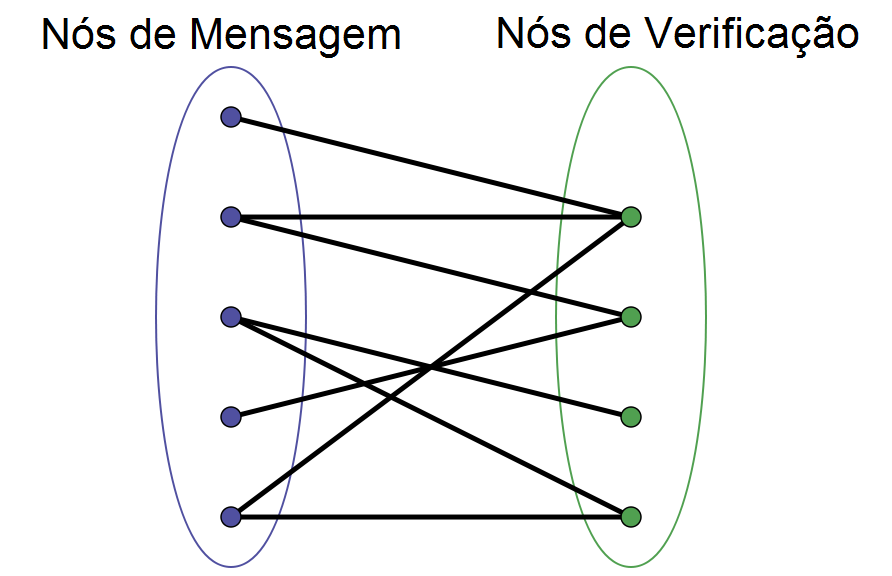
\includegraphics[width=0.4\textwidth]{figs/bipartite-graph.png}
	\caption{Grafo bipartido}
	\label{fig:bipartite-graph}
\end{figure}

A representação por grafos é análoga a representação matricial olhando para a matriz de adjacência do grafo: seja $H$ uma matriz binária $r \times n$ cuja entrada $(i, j)$ é 1 se e somente se o $i$-ésimo nó de verificação está conectado ao $j$-ésimo nó de mensagem no grafo. Então, o código LDPC definido pela grafo é o conjunto de vetores $c = (c_1, \dots, c_n)$ tal que $H \cdot c^{\tp} = 0$. A matriz $H$ é chamada de \emph{matriz de paridade} para o código. Reciprocamente, qualquer matriz binária $r \times n$ da origem a um grafo bipartido entre $n$ nós de mensagens e $r$ nós de verificação, e o código definido como espaço nulo de $H$ é precisamente o código associado a esse grafo. Portanto, qualquer código linear possui uma representação tal como um código associado a um grafo bipartido (note que esse grafo não é definido unicamente pelo código). Entretanto, nem todo código linear binário possui uma representação como um grafo bipartido \emph{esparso}. Se existir, então o código é chamado de código de verificação de paridade de baixa densidade (\emph{low-density parity-check}, ou LDPC).

Uma importante subclasse dos códigos LDPC que apresentam vantagens sobre outros códigos da mesma classe é o dos códigos de verificação de paridade de baixa densidade quase-cíclicos (QC-LDPC)~\cite{tanner}. Em geral, um código QC-LDPC $[n, k]$ satisfaz $n = n_0 b$ e $k = k_0 b$ (e assim também $r = r_0 b$) para algum $b$, $n_0$, $k_0$ (e $r_0$), e admite uma matriz de paridade que consiste de $n_0 \times r_0$ blocos de submatrizes circulantes esparsas $b \times b$. Um caso particular importante é quando $b = r$ (e também $r_0 = 1$ e $k_0 = n_0 - 1$), uma vez que uma matriz de paridade sistemática para esse código é totalmente definido pela primeira linha de cada bloco $r \times r$. Diz-se que a matriz de paridade está na \emph{forma circulante}.


Contudo, mostrou-se que todas essas propostas contêm vulnerabilidades que as tornam inadequadas para fins criptográficos~\cite{otmani-tillich-dallot}. Com efeito, o alçapão nesses métodos era protegido essencialmente por nenhum outro mecanismo além de uma permutação privada do código subjacente. A estratégia de ataque nesse panorama consiste em obter um sistema solúvel de equações lineares que os componentes da matriz de permutação precisa satisfazer, e foi montada com sucesso devido à natureza excessivamente restritiva da permutação secreta (uma vez que ela precisa preservar a estrutura quase-cíclica do resultado) e ao fato de que o código secreto é um subcódigo muito particular de um código público.

Uma tentativa de consertar a proposta de Baldi e Chiaraluce chegou a ser proposta~\cite{baldi-chiaraluce-bodrato}. Mais recentemente, Berger \emph{et al}.~\cite{berger-cayrel-gaborit-otmani} mostraram como evitar os problemas do esquema original de Gaborit e remover as vulnerabilidades até então conhecidas por meio de duas técnicas: 
\begin{enumerate}
	\item Extrair códigos públicos encurtados por blocos de códigos privados muito longos, explorando um teorema devido a Wieschebrink sobre a $NP$-completeza de distinguir códigos encurtados~\cite{wieschebrink};
	\item Trabalhar com subcódigos de subcorpo sobre um corpo intermediário entre o corpo e o corpo de extensão do código GRS original adotado pela construção.
\end{enumerate}
Essas técnicas foram aplicadas com algum sucesso a códigos quase-cíclicos. Contudo, a quase totalidade dessa família de códigos foi posteriormente quebrada devido a falhas estruturais de segurança, mais precisamente uma relação entre a estrutura secreta e certos sistemas de equações multivariadas quadráticas~\cite{faugere-otmani-perret-tillich}.

A sabedoria histórica e experimental sugere, portanto, restringir a busca de \\parâmetros mais eficientes para criptossistemas baseados em códigos à classe dos códigos de Goppa.

\subsection{Códigos MDPC e QC-MDPC}\label{subsec:qcmdpc}

Uma subclasse interessante em termos de criptografia da família QC-LDPC é dos códigos de verificação de paridade de densidade moderada (MDPC) e sua variante quase-cíclica (QC-MDPC)~\cite{misoczki-sendrier-tillich-barreto}.

Esses códigos, apresentados por Misoczki \emph{et al.}, possuem densidades próximas o bastante de códigos LDPC que possibilitam a decodificação pelos métodos simples (e indiscutivelmente mais eficientes) de propagação de crença e \emph{bit flipping} de Gallager, ainda denso o bastante para prevenir ataques baseados na presença de palavras muito esparsas no código dual como visto no ataque Stern~\cite{stern} e algumas variantes, sem perder muita capacidade de correção de erros, bem como manter ataques de decodificação baseados em conjuntos de informações~\cite{bernstein-lange-peters,bernstein-lange-peters:bcd} também inviáveis. 

Além disso, para prevenir ataques estruturais como proposto por Faug\`{e}re \\\emph{et al.}~\cite{faugere-otmani-perret-tillich} e por Leander e Gauthier~\cite{gauthier-leander}, códigos orientados a criptografia devem se manter o máximo possível sem estrutura, exceto para o alçapão secreto que permite a decodificação privada e, no caso de códigos quase-cíclicos, simetrias externas que permitam uma implementação eficiente. Finalmente, a simetria circulante pode introduzir fraquezas de segurança como apontada por Sendrier~\cite{sendrier-doom}, mas isso induz somente um ganho polinomial (especificamente, linear) em eficiência de ataques, e um pequeno ajuste nos parâmetros elimina totalmente esse problema. Densidades típicas nesse caso estão no intervalo de 0.4\% a 0.9\% do tamanho do código, uma ordem de magnitude acima de códigos LDPC, mas bem abaixo dos publicados em MDPC mencionados acima, e certamente dentro da margem estipulada para códigos de Gallager. A construção é também tão aleatória quanto possível, apenas mantendo a densidade desejada e a geometria circulante, além do tamanho do código ser muito maior que valores típicos para MDPC.

\subsection{Método de Decodificação de decisão abrupta de Gallager (\emph{Bit Flipping})}\label{subsec:hdd-recap}

Nessa seção descrevemos o algoritmo de Gallager (\emph{Gallager's hard decision decoding algorithm}, ou mais simplesmente \emph{bit flipping}, seguindo a concisa e clara descrição de Huffman e Pless~\cite{huffman-pless}. Algoritmo esse necessário para recuperar a mensagem original a partir da palavra de código encriptada com erros.

Assumindo que a palavra de código é encriptada com um código binário LDPC $\mathscr{C}$ para transmissão, e o vetor $c$ é recebido. Para o cálculo da síndrome $s = c H^{\tp}$, cada bit recebido de $c$ afeta no máximo $d_v$ componentes dessa síndrome. Se somente o $j$-ésimo bit de $c$ contiver um erro, então o correspondente $d_v$ de componente $s_i$ de $s$ será igual a 1, indicando as equações de verificação de paridade que não estão satisfeitas. Mesmo se tiver alguns outros bits com erro entre aqueles que contribuíram para o cálculo de $s_i$, espera-se que vários dos $d_v$ componentes de $s$ serão iguais a 1. Essa é a base do algoritmo de decodificação de Gallager, tanto \textit{hard decision decoding}, quanto \textit{bit-flipping}.

\begin{enumerate}
	\item Computar $c H^{\tp}$ e determinar as posições de paridade que estão insatisfeitas (pode-se dizer que essas posições são os componentes de $c H^{\tp}$ iguais a 1). \label{step:syndrome}
	\item Para cada um dos $n$ bits, computar o número de posições de paridade insatisfeitas que envolvem aquele bit. \label{step:count-unsat}
	\item Inverta o valor dos bits de $c$ que estão envolvidos no maior número de posições insatisfeitas. \label{step:threshold}
	\item Repetir passos \ref{step:syndrome}, \ref{step:count-unsat}, e \ref{step:threshold} até que se tenha $c H^{\tp} = 0$, no caso que $c$ foi decodificado com sucesso, ou até que um certo limite de número de iterações seja alcançado, para o caso que a decodificação do vetor recebido falhou.
\end{enumerate}

O algoritmo de \emph{bit-flipping} não é o melhor método de decodificação para códigos LDPC; de fato, a técnica de propagação de crença~\cite{gallager,huffman-pless}, é conhecida por exceder sua capacidade de correção de erros. Entretanto, decodificadores de propagação de crença envolvem uma computação com uma \emph{probabilidade} cada vez mais refinada para cada bit da palavra recebida $c$ que contiver um erro, incorrendo em aritmética de ponto flutuante ou aproximações de alta precisão que se adequem ao processo e algoritmos computacionalmente caros. Em um cenário em que o número de erros é fixo e conhecido antecipadamente, como é o caso de aplicações criptográficas, parâmetros podem ser ajustados de tal forma que métodos de decodificação complexos e caros, como a propagação de crença, não são mais necessários.

\subsection{Assinaturas digitais com códigos corretores de erros}\label{subsec:sighcode}

Após algumas tentativas falhas de se criar um esquema de assinatura digital \\baseada em códigos corretores de erros~\cite{alabbadi-wicker,stern-sign}, em 2001, Courtois, Finiasz e Sendrier propuseram um esquema promissor~\cite{courtois-finiasz-sendrier}.

\subsubsection{CFS}\label{subsubsec:cfs}

O \emph{CFS} foi proposto como um Sistema de Assinaturas Digitais baseado no Sistema Criptográfico McEliece. Por definição, um sistema de assinatura digital deve prover uma maneira de assinar qualquer documento de tal forma que identifique unicamente seu autor e que disponha de um algoritmo público eficiente de verificação de asssinatura. Para essas tarefas, deve ser escolhido um código linear, ilustrado na explicação como $\mathcal{C}$. Então, o CFS usa uma função de hash pública para resumir o documento \emph{m} a ser assinado no vetor $h(m)$. Decodificando esse hash com o algoritmo de correção de erros do código escolhido, obtemos um vetor \emph{c'}, correspondendo a assinatura da mensagem $m$. Para a verificação da assinatura, basta encriptar $c'$, recebido junto da mensagem $m$, e verificar se corresponde ao cálculo do hash da mensagem $m$. Como podemos verificar abaixo:

\begin{itemize}
    \item Geração de Chaves
    \begin{enumerate}
        \item Escolher um Código de Goppa $G(L,g(X))$
        \item Obter sua matriz $(n - k) \times n$ de verificação de paridade $H$
        \item Calcular $V = SHP$, onde $S$ é uma matriz binária inversível $(nk) \times (nk)$ aleatória e $P$ uma matriz de permutação aleatória $n \times n$.
    \end{enumerate}
    Assim, as chaves seriam: Chave Privada = $G$, Chave Pública = $(V,t)$.
    
    \item Assinatura
    \begin{enumerate}
        \item Encontrar o menor $i \in \mathbb{N}$ tal que, para $c = h(m,i)$ e $c' = S^{-1}c$, $c'$ seja uma síndrome decodificável de $G$.
        \item Usando o algoritmo de decodificação de $G$, obter o vetor de erros $e'$, cuja síndrome seja $c'$, ou seja $c' = H(e')^t$.
        \item Obter $e^t = P^{-1}(e')^t$.
    \end{enumerate}
    Assim, a assinatura é o par: $(e,i)$.
    
    \item Verificação de Assinatura
    \begin{enumerate}
        \item Obter $c = Ve^t$.
        \item Aceite somente se $c = h(m,i)$
    \end{enumerate}
\end{itemize}

Apesar do CFS ser um esquema de assinatura ainda seguro após passar por várias criptoanálises, não é adequado para aplicações padrão comumente utilizadas hoje, já que além do tamanho das chaves públicas o custo para assinar são muito grandes para um conjunto de parâmetros seguros.


%%%%%%%%%%%%%%%%%%%%%%%%%%%%%%%%%%%%%%%%%%%%%%%%%
\section{Criptografia baseada em reticulados}
%%%%%%%%%%%%%%%%%%%%%%%%%%%%%%%%%%%%%%%%%%%%%%%%%

O uso de reticulados em criptografia surgiu com o trabalho de Ajtai~\cite{ajtai}, onde o problema de encontrar vetores pequenos em uma classe aleatória de reticulados é utilizado como base da demonstração da existência de funções de mão única. A criptografia baseada em reticulados, além de estar amparada por demonstrações de segurança construídas sobre a dificuldade do pior caso de determinados problemas, possui implementações eficientes e descrições relativamente simples de serem compreendidas.

%NOVO: 17/09 23:05
A criptografia baseada em reticulados pode ser dividida em duas categorias: (i) com demonstração de segurança, como por exemplo o esquema de Ajtai ou aqueles com base no problema LWE, cujos algoritmos envolvem operações com uma matriz $A$, que, como veremos adiante, está associada a chave pública, fazendo com que a encriptação e decriptação tenham complexidade quadrática ou mesmo cúbica, deixando a desejar em relação a criptografia convencional; ou (ii) sem demonstração de segurança, porém com implementação eficiente, como o NTRU. Um desafio recentemente resolvido foi o de prover demonstração de segurança, com base no pior caso de problemas em reticulados ideais, para esquemas com performance semelhante ao NTRU~\cite{Stehle2011}. Embora problemas intratáveis em reticulados possam não ser intratáveis em reticulados ideais, não é conhecido nenhum algoritmo polinomial para resolvê-los, mesmo com fator de aproximação polinomial ou com o uso de computadores quânticos.

\subsection{Fundamentos}

\begin{definition}
Formalmente, reticulados são definidos como a combinação linear de $n$ elementos $b_1, ...,b_n \in \mathbb{R}^m$, linearmente independentes, denominados \textit{base do reticulado}.  

$$\mathcal{L}(b_1,...,b_n) = \left\{\sum_{i=1}^{n} x_ib_i : x_i \in \mathbb{Z}\right\}. $$
\end{definition}

Em outras palavras, um reticulado é um espaço vetorial discretizado, ou seja, existe uma analogia que nos permite utilizar conceitos como norma, dimensão, ortogonalidade, transformação linear, entre outros. Uma maneira alternativa de abordar o assunto é por meio de notação matricial, onde a base pode ser representada por uma matriz $B = [b_1, ..., b_n]$, pertencente a $\mathbb{R}^{m \times n}$. 
O reticulado gerado pela matriz $B$ é definido por $\mathcal{L} = \left\{ Bx \mid x \in \mathbb{Z}^n \right\}$, de forma que o determinante $\det{(B)}$ é independente da escolha da base e corresponde geometricamente ao inverso da densidade de pontos do reticulado em $\mathbb{Z}^m$.  

\begin{definition}
Dado um reticulado $\mathcal{L}(B)$, os vetores que constituem a base do reticulado podem ser encarados como arestas de um paralelepípedo de dimensão $n$. Assim, podemos definir $\mathcal{P}(B) = \{Bx \mid x \in [0,1)^n\}$, denominado \textit{paralelepípedo fundamental} de $B$. 
Podemos redefinir o paralelepípedo de forma a obter uma região simétrica. Para isso, seja $\mathcal{P}_{1/2}(B) = \{Bx \mid x \in [-1/2,1/2)^n\}$, denominado \textit{paralelepípedo fundamental centralizado} de $B$. As figuras \ref{fundamental} e \ref{fundamentalc} ilustram exemplos de paralelepípedos fundamentais (centralizado ou não) em dimensão 2.  
\end{definition}


\begin{figure}[ht]
\begin{center}
\begin{multicols}{2}
\begin{tikzpicture}
\draw[->] (-0.4,0) -- (4.2,0) node[right] {};
    \draw[->] (0,-0.4) -- (0,4.2) node[above] {};

    \fill (0, 0) circle[radius=0.5pt];
	\fill (0.125, 1.125) circle[radius=1pt];
	\fill (0.250, 2.250) circle[radius=1pt];
	\fill (0.375, 3.375) circle[radius=1pt];
	
	\fill (1.125, 0.125) circle[radius=1pt];
	\fill (1.250, 1.250) circle[radius=1pt];
	\fill (1.375, 2.375) circle[radius=1pt];
	\fill (1.500, 3.500) circle[radius=1pt];

	\fill (2.250, 0.250) circle[radius=1pt];
	\fill (2.375, 1.375) circle[radius=1pt];
	\fill (2.500, 2.500) circle[radius=1pt];
	\fill (2.625, 3.625) circle[radius=1pt];

	\fill (3.375, 0.375) circle[radius=1pt];
	\fill (3.500, 1.500) circle[radius=1pt];
	\fill (3.625, 2.625) circle[radius=1pt];
	\fill (3.750, 3.750) circle[radius=1pt];

    \draw[gray, fill=gray] (0,0) -- (1.125, 0.125) -- (1.250, 1.250) -- (0.125,1.125);
    \draw[->] (0,0) -- (1.125, 0.125) node[right] {$v_1$};
    \draw[->] (0,0) -- (0.125,1.125) node[above] {$v_2$};
    \node at (0.625,0.625) {};
\end{tikzpicture}
\caption{$\mathcal{P}(B)$}
\label{fundamental}
\begin{tikzpicture}
\draw[->] (-1.4,0) -- (3.2,0) node[right] {};
    \draw[->] (0,-1.4) -- (0,3.2) node[above] {};

	\fill (0, 0) circle[radius=0.5pt];
	\fill (0.125, 1.125) circle[radius=1pt];
	\fill (0.250, 2.250) circle[radius=1pt];
	\fill (0.375, 3.375) circle[radius=1pt];
	
	\fill (1.125, 0.125) circle[radius=1pt];
	\fill (1.250, 1.250) circle[radius=1pt];
	\fill (1.375, 2.375) circle[radius=1pt];
	\fill (1.500, 3.500) circle[radius=1pt];

	\fill (2.250, 0.250) circle[radius=1pt];
	\fill (2.375, 1.375) circle[radius=1pt];
	\fill (2.500, 2.500) circle[radius=1pt];
	\fill (2.625, 3.625) circle[radius=1pt];

	\fill (-1.125, -0.125) circle[radius=1pt];
	\fill (-1.000, 1.000) circle[radius=1pt];
	\fill (-0.875, 2.125) circle[radius=1pt];
	\fill (-0.750, 3.250) circle[radius=1pt];

    \draw[gray, fill=gray] (-0.625,-0.625) -- (-0.500, 0.500) -- (0.625, 0.625) -- (0.500,-0.500) -- (-0.625,-0.625);
    \draw[->] (0,0) -- (1.125, 0.125) node[right] {$v_1$};
    \draw[->] (0,0) -- (0.125,1.125) node[above] {$v_2$};
    \draw[-] (-0.625,-0.625) -- (-0.500, 0.500) node[] {};
    \draw[-] (-0.625,-0.625) -- (0.500,-0.500) node[] {};
    \node at (0.625,0.625) {};
\end{tikzpicture}
\caption{$\mathcal{P}_{1/2}(B)$}
\label{fundamentalc}
\end{multicols}
\end{center}
\end{figure}

\begin{theorem}
\label{redLat}
Seja $\mathcal{L} \in \mathbb{R}^m$ um reticulado de dimensão $n$ e seja $\mathcal{F}$ o paralelepípedo fundamental de $\mathcal{L}$, então dado um elemento $w \in \mathbb{R}^m$, podemos escrever $w$ na forma $w = v + t$, para $v \in \mathcal{L}$ e $t \in \mathcal{F}$ únicos. Esta equação pode ser encarada como uma redução modular, onde o vetor $t$ é interpretado como $w \pmod{\mathcal{F}}$. 
\end{theorem}


\begin{figure}[ht]
\begin{center}
\begin{tikzpicture}
\draw[->] (-0.4,0) -- (4.2,0) node[right] {};
    \draw[->] (0,-0.4) -- (0,4.2) node[above] {};

	\fill (0, 0) circle[radius=0.5pt];
	\fill (0.125, 1.125) circle[radius=1pt];
	\fill (0.250, 2.250) circle[radius=1pt];
	\fill (0.375, 3.375) circle[radius=1pt];
	
	\fill (1.125, 0.125) circle[radius=1pt];
	\fill (1.250, 1.250) circle[radius=1pt];
	\fill (1.375, 2.375) circle[radius=1pt];
	\fill (1.500, 3.500) circle[radius=1pt];

	\fill (2.250, 0.250) circle[radius=1pt];
	\fill (2.375, 1.375) circle[radius=1pt];
	\fill (2.500, 2.500) circle[radius=1pt];
	\fill (2.625, 3.625) circle[radius=1pt];

	\fill (3.375, 0.375) circle[radius=1pt];
	\fill (3.500, 1.500) circle[radius=1pt];
	\fill (3.625, 2.625) circle[radius=1pt];
	\fill (3.750, 3.750) circle[radius=1pt];

    \draw[gray, fill=gray] (0,0) -- (1.125, 0.125) -- (1.250, 1.250) -- (0.125,1.125);

    \fill (3.150, 0.900) circle[radius=1pt];
    \draw[->] (0,0) -- (2.250,0.250) node[below] {$v$};
    \draw[->] (0,0) -- (3.150,0.900) node[above] {$w$};
    \draw[->] (2.250,0.250) -- (3.150,0.900) node[above] {};
    \draw[->] (0,0) -- (0.900,0.650) node[left] {$t$}; 
    \draw[->] (0.900,0.650) -- (3.150,0.900) node[above] {};
    \node at (0.625,0.625) {};
\end{tikzpicture}
\caption{Redução módulo $\mathcal{P}(B)$}
\label{fig2}
\end{center}
\end{figure}


O volume do paralelepípedo fundamental é dado por $\Vol(\mathcal{F}) = |\Det(B)|$. Dadas duas bases $B = \{b_1, ..., b_n\}$ e $B' = \{b'_1, ..., b'_n\}$ de um mesmo reticulado $\mathcal{L}$, temos que $\Det(B) = \pm\Det(B')$. 

O problema de encontrar o vetor de norma mínima (\emph{shortest vector problem} - SVP) é uma das questões fundamentais em reticulados. Rigorosamente, dado o reticulado $\mathcal{L}(B)$, deseja-se encontrar o vetor não nulo com norma mínima. Na prática, é utilizado um fator de aproximação $\gamma(n)$ para o problema SVP, isto é, deseja-se encontrar um vetor cuja norma seja inferior ao vetor de norma mínima, multiplicada por $\gamma(n)$. 

%%Ajtai demonstrou que o SVP é NP-difícil para uma classe aleatória de reticulados~\cite{ajtai}. Em 1998, Micciancio \cite{Micciancio98onthe} provou que o problema SVP é NP-difícil para um fator de aproximação inferior a $\sqrt{2}$, utilizando norma euclidiana. Posteriormente, o fator de aproximação foi aprimorado, obtendo $\gamma(n) = n^{O(1/\log \log n)}$ \cite{Khot00inapproximabilityresults}. Por outro lado, para fatores de aproximação superiores a $\sqrt{n/\log n}$, existem indícios fortes de que o problema SVP não é NP-difícil \cite{Aharonov}.

Outros problemas em reticulados, importantes do ponto de vista da criptografia, são:

\begin{itemize}
\item o \textit{problema do vetor de distância mínima} (\emph{closest vector problem} - CVP). Dados um reticulado $\mathcal{L}(B)$ e um vetor $t \in \mathbb{R}^m$, o objetivo é encontrar o vetor $v \in \mathcal{L}(B)$ que seja mais próximo de $t$;

\item e o \textit{problema dos vetores independentes mínimos} (\emph{shortest independent vector problem} - SIVP). Dada uma base $B \in \mathbb{Z}^{m \times n}$, o problema consiste em encontrar $n$ vetores linearmente independentes $(v_1, ..., v_n)$, pertencentes ao reticulado, tais que a norma máxima entre os vetores $v_i$ seja mínima.
\end{itemize}

\begin{definition}
Dado um reticulado $\mathcal{L}$ e uma base $B = (v_1, ...v_n)$, a \textit{razão de Hadamard}, denotada por $\mathcal{H}(B)$, é definida da seguinte maneira:

$$\mathcal{H}(B) = \left( \frac{\Det \mathcal{L}}{\prod_{1 \leq i \leq n} ||v_i|| } \right)^{1/n}.$$
\end{definition}

É fácil mostrar que, para qualquer base $B$, temos que $0 \leq \mathcal{H}(B) \leq 1$. Além disso, 
quanto mais próximo de 1 mais ortonormal é a base.

Uma classe particularmente importante de reticulados é aquela formada pelos \textit{reticulados q-ários}, denotados por $\Lambda_q$. Dado um inteiro $q$, os vetores do reticulado são restritos, coordenada a coordenada, a elementos de $\mathbb{Z}_q$. Dada uma matriz $A \in \mathbb{Z}_q^{n \times m}$, o reticulado q-ário é determinado pelas linhas de $A$, ao invés das colunas. Ou seja, é formado pelos vetores $y = A^Ts \pmod q$, para $s \in \mathbb{Z}^n$. O reticulado q-ário ortogonal, $\Lambda_q^\perp$, em relação a matriz $A$, é dado pelos vetores $y$ tais que $Ay=0 \pmod q$. Dado um reticulado $\mathcal{L}$, o \textit{reticulado dual}, $\mathcal{L}^*$, é formado pelos vetores $y$, tais que $\langle x,y \rangle \in \mathbb{Z}$, para $x \in \mathcal{L}$. Em especial, o reticulado q-ário ortogonal, $\Lambda_q^\perp(A)$, é igual a $q\Lambda_q(A)^*$.

\subsubsection{Algoritmo LLL}

Nesta seção será descrito o algoritmo LLL, que calcula uma nova base para um determinado reticulado, com razão de Hadamard mais próxima a 1. Isto é, o algoritmo LLL realiza o que chamamos de redução de base, porque os vetores da nova base tem maior ortonormalidade que a base original. Portanto, este algoritmo pode ser utilizado para resolver o problema SVP, como veremos adiante. 

Em um espaço vetorial com base $(v_1, \cdots, v_n)$, a obtenção de uma base ortonormal é realizada pelo algoritmo Gram-Schmidt. A ideia da redução de Gauss é a mesma que está por trás do algoritmo Gram-Schmidt, onde temos que $\mu_{ij} = v_iv_j^*/||v_j^*||^2$, mas os valores de $\mu_{ij}$ não são necessariamente inteiros, de modo que a redução de Gauss considera o uso do inteiro mais próximo $\lfloor \mu_{ij} \rceil$. O algoritmo termina quando este inteiro mais próximo é zero, condição que apenas em dimensão 2 garante que o menor vetor foi encontrado. 

\begin{algorithm}
\caption{Redução de Gauss}
\label{gauss}
\begin{algorithmic}
\Require Uma base $(v_1,v_2)$.
\Ensure Retorna uma base com o menor vetor do reticulado ($v^*_1$) e com um vetor $v^*_2$ que não pode ser reduzido pela subtração de $v_1$.
\State $v_1^* = v_1$ e $v_2^* = v_2$.
\While {verdade}
\If {$||v^*_2|| < ||v^*_1||$}
\State troque $v_1^*$ com $v_2^*$
\EndIf
\State Calcule $m = \lfloor v_1^*.v_2^*/||v^*_1||^2 \rceil$.
\If {$m=0$}
\Return $(v^*_1,v_2^*)$.
\EndIf
\State Troque $v_2^*$ por $v_2^* - mv^*_1$.
\EndWhile

\end{algorithmic}
\end{algorithm}

\begin{definition}
Seja $B = (v_1, ..., v_n)$ a base de um reticulado $\mathcal{L}$ e seja $B^* = (v_1^*, ..., v_n^*)$ a base retornada pelo algoritmo Gram-schmidt. A base $B$ é denominada \textit{LLL reduzida} se forem satisfeitas as seguintes condições:

\textbf{Condição de norma:} $|\mu_{i,j}| = \frac{v_i.v_j^*}{||v^*_{j}||^2} \leq \frac{1}{2}$ para todo $1 \leq j < i \leq n$.

\textbf{Condição de Lovász:} $||v_i^*||^2 \geq (\frac{3}{4} - \mu_{i,i-1}^2) ||v_{i-1}^*||^2$ para todo $1 < i \leq n$.
\end{definition}

\begin{theorem}
Seja $B$ uma base LLL reduzida de um reticulado $\mathcal{L}$, então $B$ resolve o problema SVP com fator de aproximação $2^{(n-1)/2}$. 
\end{theorem}

Um ponto importante que merece destaque é a escolha do valor $3/4$. Se este valor fosse substituído por $1$,  obteríamos a redução de Gauss. Porém, não se sabe se o algoritmo iria terminar em tempo polinomial. Na verdade, qualquer valor estritamente menor que $1$ faz com que o algoritmo termine em tempo polinomial. Com isso, criptossistemas baseados em problemas como SVP e CVP devem ter seus parâmetros ajustados para evitar ataques que utilizam o algoritmo LLL.

\begin{algorithm}
\caption{LLL}
\begin{algorithmic}
\Require Uma base $(v_1, ..., v_n)$.
\Ensure Retorna uma base com o menor vetor do reticulado ($v^*_1$) e com um vetor $v^*_2$ que não pode ser reduzido pela subtração de $v_1$.
\State $k=2$.
\State $v_1^* = v_1$.
\While {$k \leq n$}
\For {$j=1$ até $j=k-1$}
\State $v_k = v_k - \lfloor\mu_{k,j}\rceil v^*_j$.
\EndFor
\If {$||v_k^*||^2 \geq (\frac{3}{4} - \mu^2_{k,k-1}) ||v^*_{k-1}||$}
\State $k = k+1$.
\Else
\State Troque $v_{k-1}$ com $v_k$.
\EndIf
\EndWhile

\Return $(v_1, ..., v_n)$.
\end{algorithmic}
\end{algorithm}

Em linhas gerais, dada uma base $(v_1, ..., v_n)$, é possível obter uma nova base satisfazendo a condição de tamanho, simplesmente subtraindo de $v_k$ múltiplos de $v_1, ..., v_{k-1}$ de modo a reduzir o valor absoluto de $v_k$. Se a condição de norma for satisfeita, verifica-se se a condição de Lovász também é satisfeita, caso não seja, os vetores são reordenados e novamente realiza-se a redução de norma. 

\subsection{Hash baseado em reticulados}

O primeiro criptossistema baseado em reticulados foi proposto por Ajtai~\cite{ajtai}. Este trabalho tem grande importância porque a demonstração de segurança foi realizada com base no pior caso de problemas em reticulados. Isto é, inverter a função de hash em média tem a mesma dificuldade que o pior caso do problema SVP em reticulados q-ários duais. 

Especificamente, dados os inteiros $n,m,d,q$, é construída uma família de hash criptográficos, $f_A : \{0,...,d-1\}^m \rightarrow \mathbb{Z}_q^n$, indexada pela matriz $A \in \mathbb{Z}_q^{n \times m}$. Dado um vetor $y$, temos que $f_A(y) = Ay \pmod q$. O algoritmo \ref{ajtai} detalha essas operações. Uma escolha possível para os parâmetros é $d=2, q=n^2, m \approx 2n \log q / \log d$, de modo a obter um fator de compressão de 2. 

A segurança do esquema está no fato de que encontrar uma colisão $f_A(y) = f_A(y')$, implica na existência de um vetor pequeno, $y-y'$, no reticulado $\mathcal{L}_q^*(A)$.

\begin{algorithm}
\begin{algorithmic}
\Require Inteiros $n, m, q, d \geq 1$. Uma matriz $A$ escolhida uniformemente em $\mathbb{Z}_q^{n \times m}$. Um vetor $y \in \{0, ..., d-1\}^m$.
\Ensure Um vetor $f(y) \in \mathbb{Z}^n_q$. 

\Return $f(y) = A.y \pmod q$.
\end{algorithmic}
\caption{Hash de Ajtai}
\label{ajtai}
\end{algorithm}

Esta proposta é bastante simples e pode ser implementada eficientemente, porém, na prática, as funções de hash são projetadas de forma \emph{ad-hoc}, sem as garantias fornecidas por uma demonstração de segurança, sendo assim mais eficientes que a construção de Ajtai. Além disso, com uma quantidade suficientemente grande de valores da função, um adversário consegue reconstruir o paralelepípedo fundamental do reticulado $\mathcal{L}_q^*(A)$, permitindo encontrar colisões facilmente. 
%NOVO: 18/09 00:43
Em 2011, Stehlé e Steinfeld~\cite{Stehle2011} propuseram uma família mais eficiente de funções de hash resistentes a colisão, cuja construção será importante para esquemas de assinatura digital, como veremos adiante. 

\subsection{Encriptação baseada em reticulados}

\subsubsection{GGH}

O criptossistema GGH~\cite{Goldreich-Goldwasser-Halevi} permite compreender facilmente o uso de reticulados no contexto de criptografia de chave pública. Este criptossistema utiliza o conceito de ortonormalidade da base na definição do par de chaves. A chave privada é definida como uma base $B_\mathrm{priv}$ do reticulado, formada por vetores quase ortogonais e com norma pequena. 


De modo geral, o criptossistema GGH funciona da seguinte maneira:

\begin{itemize}
 
\item o algoritmo de encriptação acrescenta o ruído $r \in \mathbb{R}^n$ ao texto claro $m \in \mathcal{L}$, gerando o texto encriptado $c = m + r$;

\item o algoritmo de decriptação precisa ser capaz de retirar o ruído inserido. Alternativamente, é preciso resolver uma instância do problema CVP.

\end{itemize}

A figura \ref{figbaseboa} mostra um reticulado em dimensão 2, com base dada pelos vetores $v_1$ e $v_2$, praticamente ortogonais. Já a figura \ref{figbaseruim} mostra uma base para o mesmo reticulado, composta por vetores pouco ortogonais.


\begin{figure}[h]
\begin{center}
\begin{multicols}{2}
\begin{tikzpicture}[scale=2]
\draw[->] (-0.4,0) -- (2.2,0) node[right] {};
    \draw[->] (0,-0.4) -- (0,2.2) node[above] {};

\foreach \x in {0,0.5, 1.0, 1.5, 2.0} {
    \foreach \y in {-0.5, 0, 0.5, 1.0, 1.5, 2.0} {
        \fill (\x,\y) circle[radius=0.5pt];
	\fill (\x-0.5/4, \y+0.5/4) circle[radius=0.5pt];
	\fill (\x-1/4, \y+1/4) circle[radius=0.5pt];
	\fill (\x-1.5/4, \y+1.5/4) circle[radius=0.5pt];
    }
}

    \draw[->] (0,0) -- (0.250, 0.250) node[above] {$v_1$};
    \draw[->] (0,0) -- (0.125,-0.125) node[above] {$v_2$};
\end{tikzpicture}
\caption{Base boa}
\label{figbaseboa}
\begin{tikzpicture}[scale=2]
\draw[->] (-0.4,0) -- (2.2,0) node[right] {};
    \draw[->] (0,-0.4) -- (0,2.2) node[above] {};

\foreach \x in {0,0.5, 1.0, 1.5, 2.0} {
    \foreach \y in {-0.5, 0, 0.5, 1.0, 1.5, 2.0} {
        \fill (\x,\y) circle[radius=0.5pt];
	\fill (\x-0.5/4, \y+0.5/4) circle[radius=0.5pt];
	\fill (\x-1/4, \y+1/4) circle[radius=0.5pt];
	\fill (\x-1.5/4, \y+1.5/4) circle[radius=0.5pt];
    }
}

    \draw[->] (0,0) -- (1.375, 0.125) node[above] {$v_1$};
    \draw[->] (0,0) -- (0.500, 0.0) node[below] {$v_2$};
\end{tikzpicture}
\caption{Base ruim}
\label{figbaseruim}
\end{multicols}
\end{center}
\end{figure}


Conforme menor a ortonormalidade da base conhecida e maior a dimensão do reticulado, mais difícil é o problema CVP. 
Desta forma, a chave pública pode ser definida por uma base $B_\mathrm{pub}$ do reticulado, tal que
$\mathcal{H}(B_\mathrm{pub})$ seja aproximadamente zero. Por outro lado, com o conhecimento da chave privada $B_\mathrm{priv}$, 
o algoritmo de Babai \cite{Babai86onlovasz}, definido a seguir, pode ser utilizado para recuperar o texto claro.

\begin{algorithm}[b]
\caption{Algoritmo de Babai}
\begin{algorithmic}
\Require o reticulado $\mathcal{L}$ de dimensão $n$; o vetor $c_{B_\mathrm{pub}} = (c_1, ..., c_n)$, onde $c_i \in \mathbb{R}$; 
e uma base $B_\mathrm{priv} = (s_1, ..., s_n)$, suficientemente ortonormal.
\Ensure o vetor $m \in \mathcal{L}$ que resolve o problema CVP com relação a $c$ e $\mathcal{L}$.
\State Resolva um sistema de $n$ equações, $c = t_1s_1 + ... + t_ns_n$, nas variavéis $t_i$, onde $1 \leq i \leq n$.
\For {$i = 0$ até $i = n$}
\State $a_i \leftarrow \lfloor t_i \rceil$
\EndFor 

\Return $m \leftarrow a_1s_1 + ... a_ns_n$
\end{algorithmic}
\end{algorithm}

A ideia geral do algoritmo de Babai é representar o vetor $c$ na base privada $B_\mathrm{priv}$, resolvendo um sistema de $n$ equações lineares. Como $c \in \mathbb{R}^{n \times n}$, para obter um elemento do reticulado $\mathcal{L}$, cada coeficiente $t_i \in \mathbb{R}^n$ é aproximado 
para o inteiro mais próximo $a_i$, onde esta operação de arredondamento é denotada por $a_i  \leftarrow \lfloor t_i \rceil$. Este procedimento simples funciona bem desde que a base $B_\mathrm{priv}$ seja suficientemente ortonormal, reduzindo os erros do arredondamento.  

\begin{figure}[h]
\begin{center}
\begin{tikzpicture}
\draw[->] (-0.4,0) -- (4.2,0) node[right] {};
    \draw[->] (0,-0.4) -- (0,4.2) node[above] {};

\foreach \x in {0,0.5, 1.0, 1.5, 2.0, 2.5, 3.0, 3.5, 4} {
    \foreach \y in {-0.5, 0, 0.5, 1.0, 1.5, 2.0, 2.5, 3.0, 3.5} {
        \fill (\x,\y) circle[radius=0.5pt];
	\fill (\x-0.5/4, \y+0.5/4) circle[radius=0.5pt];
	\fill (\x-1/4, \y+1/4) circle[radius=0.5pt];
	\fill (\x-1.5/4, \y+1.5/4) circle[radius=0.5pt];
    }
}

    \draw[->] (0,0) -- (3.0, 1) node[below] {$v_1$};
    \draw[->] (0,0) -- (3.0, 1.5) node[above] {$v_2$};
    \draw[->] (3.0, 1) -- (6.0, 2.5) node[above] {};
    \draw[->] (3.0, 1.5) -- (6.0, 2.5) node[above] {};
    \fill (3.1,1.17) circle[radius=1.3pt];
\end{tikzpicture}
\caption{CVP com base ruim}
\label{figbase}
\end{center}
\end{figure}

Uma forma de atacar o criptossistema GGH é tentar melhorar a base $B_\mathrm{pub}$, ou seja, tornar seus vetores menores e mais ortogonais. Em dimensão 2 o problema pode ser facilmente resolvido usando o algoritmo de Gauss (algoritmo \ref{gauss}). Para dimensões grandes o problema é considerado difícil, mas em 1982 houve grande avanço, com a publicação do algoritmo LLL~\cite{LLL}. Sendo assim, os parâmetros do criptossistema devem ser projetados para que o algoritmo LLL não possa ser usado para resolver o problema CVP.


\subsubsection{NTRU}

O criptossistema NTRU~\cite{NTRU} é construído sobre aneis polinomiais, mas também pode ser definido com base em reticulados, isto porque o problema subjacente pode ser interpretado como sendo o SVP e o CVP. Desta maneira, a solução de algum desses problemas representaria um ataque ao criptossistema, de modo que os parâmetros devem ser ajustados para que o algoritmo LLL não possa se usado para este fim.

O criptossistema utiliza os seguintes aneis polinomiais: $R = \mathbb{Z}[x]/(x^N-1)$, $R_p = (\mathbb{Z}/p\mathbb{Z})[x]/(x^N-1)$ e $R_q = (\mathbb{Z}/q\mathbb{Z})[x]/(x^N-1)$, onde $N, p, q$ são inteiros positivos. 
 
\begin{definition}
Dados os inteiros positivos $d_1$ e $d_2$, define-se $\mathcal{T}(d_1, d_2)$ como sendo a classe de polinômios tais que existam $d_1$ coeficientes iguais a $1$, $d_2$ coeficientes iguais a $-1$ e o restante dos coeficientes iguais a zero. Estes polinômios são denominados \emph{polinômios ternários}.
\end{definition}

Os parâmetros públicos são dados por $(N, p, q, d)$, onde $N$ e $p$ são primos, $(p, q) = (N, q) = 1$ e $q > (6d+1)p$. A chave privada corresponde aos polinômios $f(x) \in \mathcal{T}(d+1,d)$ e $g(x) \in \mathcal{T}(d,d)$. A chave pública é o polinômio $h(x) \equiv F_q(x).g(x)$, onde $F_q(x)$ é o inverso multiplicativo de $f(x)$ em $R_q$.

Dada uma mensagem $m(x) \in R$, cujos coeficientes estejam no intervalo entre $-p/2$ e $p/2$, escolhe-se aleatoriamente $r(x)$ e calcula-se o texto encriptado $e(x) \equiv p h(x).r(x) + m(x) \pmod q$. 

Para decriptar, primeiramente calcula-se a função $a(x) \equiv f(x).e(x) \pmod q$, de tal modo que os coeficientes estejam entre $-q/2$ e $q/2$, para então obter novamente a mensagem $m(x)$, tal que $m(x) \equiv F_p(x).a(x) \pmod p$.

\begin{itemize}
\item \textsf{GerarChaves.}  Escolhe-se $f \in \mathcal{T}(d+1, d)$ tal que $f$ possua inversa em $R_q$  $R_p$. Escolhe-se também $g \in \mathcal{T}(d,d)$. Calcule$F_q$ como sendo o elemento inverso de $f$ em $R_q$ e, analogamente, $F_p$ o elemento inverso de $f$ em $R_p$. A chave pública é 
dada por $h = F_q.g$.  

\item \textsf{Encriptar.} Dado o texto claro $m \in R_p$, escolhe-se aleatoriamente $r \in \mathcal{T}(d,d)$ e calcule $e \equiv pr.h + m \pmod{q}$, onde $h$ é a chave pública do destinatário. 

\item \textsf{Decriptar.} Calcule $a = \lfloor f.e \equiv pg.r + f.m \rceil_q$. Finalmente, a mensagem pode ser obtida pelo cálculo $m \equiv F_p.a \pmod{p}$. 
\end{itemize}

\subsubsection{Encriptação baseada no problema LWE (Learning with Errors)}
\label{LWE}

Assim como o GGH, o NTRU não possui demonstração de segurança. Nesta seção será apresentado o criptossistema baseado no problema LWE, que é uma proposta eficiente e que possui demonstração de segurança com base no pior caso de problemas em reticulados~\cite{surveyRegev10}. Esta demonstração é uma redução quântica, isto é, mostra que uma vulnerabilidade do criptossistema implica em um algoritmo quântico para resolver problemas em reticulados. Em 2009, Peikert mostrou uma redução clássica na demonstração de segurança do problema LWE~\cite{peikert}.

\begin{definition}
O \textit{problema LWE} consiste em encontrar o vetor $s \in \mathbb{Z}_q^n$, dadas as equações $\langle s, a_i \rangle + e_i = b_i \pmod q$, para $1 \leq i \leq n$. Os valores $e_i$ são pequenos erros que são inseridos, de acordo com uma distribuição $\mathcal{D}$, geralmente tomada como sendo a distribuição normal. 
\end{definition}

Em 2010, Lyubaskevsky, Peikert e Regev usaram aneis polinomiais para definir o esquema RLWE~\cite{RingLWE}. Seja $f(x) = x^d + 1$, onde $d$ é uma potência de 2. Dado um inteiro $q$ e um elemento $s \in R_q = \mathbb{Z}_q[x]/f(x)$, o \textit{problema LWE em anel} sobre $R_q$, com relação a uma distribuição $\mathcal{D}$, é definido equivalentemente, ou seja, é preciso encontrar $s$ que satisfazendo as equações $s.a_i + e_i = b_i \pmod{R_q}$, para $1 \leq i \leq n$, onde $a_i$ e $b_i$ são elementos de $R_q$ e a redução modular em $R_q$ é o mesmo que reduzir o polinômio resultante módulo $f(x)$ e seus coeficientes módulo $q$. Assim, o criptossistema baseado no problema LWE pode ser construído da seguinte maneira:

\begin{itemize}
\item \textsf{GerarChaves.} Escolhe-se aleatoriamente $a \in R_q$ e utiliza-se a distribuição $\mathcal{D}$ para gerar $s$ e $e$ em $R$. 
A chave priva é dada por $s$, enquanto a chave pública é dada por $(a, b= a.s + e)$. 
\item \textsf{Encriptar.} Para encriptar $d$ bits, é possível interpretar esses bits como coeficientes de um polinômio em $R$. O algoritmo de encriptação então escolhe $r,e_1,e_2 \in R$, usando a mesma distribuição $\mathcal{D}$ e calcula $(u,v)$ da seguinte maneira:

\begin{align*}
u &= a.r + e_1 \pmod q \textrm{,}\\
v &= b.r + e_2 + \lfloor q/2 \rfloor .z \pmod q.
\end{align*}

\item \textsf{Decriptar.} Por sua vez, o algoritmo de decriptação calcula

\[
v - u.s = (r.e - s.e_1 + e_2) + \lfloor q/2 \rfloor .z \pmod q.
\]

\end{itemize}

De acordo com a escolha de parâmetros, temos que $(r.e - s.e_1 + e_2)$ tem tamanho no máximo $q/4$, de modo que os bits do texto claro podem ser calculados verificando cada coeficiente do resultado obtido. Se o coeficiente for mais próximo de $0$ que de $q/2$, então o bit correspondente é $0$, caso contrário é $1$. 

%NOVO: 18/09 ~1:00
Alguns conceitos desta seção, como por exemplo o uso do polinômio ciclotômico $f(x)$ e a distribuição gaussiana $\mathcal{D}$, foram recentemente incorporados ao esquema NTRU, permitindo com isso obter um esquema semanticamente seguro e eficiente para encriptação baseada em reticulados~\cite{Stehle2011}, cujas chaves pública e privada e algoritmos de encriptação e decriptação têm complexidade $\tilde{O}(\lambda)$, onde $\lambda$ é o parâmetro de segurança.

\subsubsection{Encriptação homomórfica}

Recentemente, Gentry propôs a construção de um esquema de encriptação completamente homomórfica~\cite{gentry}, resolvendo assim um problema que estava em aberto desde 1978, quando Rivest, Adleman e Dertouzos conjecturaram a existência de homomorfismos secretos~\cite{minicursoFHE}, onde a função de encriptação também é um homomorfismo algébrico. Em outras palavras, é possível somar e multiplicar textos encriptados, de modo que, ao decriptá-los, obtêm-se o resultados das mesmas operações, realizadas com o texto claro correspondente. 

Se o espaço de texto claro for dado por $\Set{0,1}$, então a soma de bits é equivalente a uma disjunção exclusiva lógica, enquanto a multiplicação é equivalente a uma conjunção lógica. Portanto, é possível computar qualquer circuito booleano sobre dados encriptados, o que permite a construção de máquinas de Turing, sendo assim possível executar homomorficamente qualquer algoritmo com argumentos encriptados, gerando uma saída encriptada. 

Utilizando a encriptação homomórfica é possível delegar a computação de algoritmos a um servidor, mantendo o sigilo dos dados de entrada. Isto é interessante para a computação em nuvem, permitindo a construção de aplicações como por exemplo banco de dados encriptado, encriptação de disco, mecanismos de busca sobre consultas encriptadas, etc. 

%A construção inicial de Gentry~\cite{gentry} foi realizada sobre reticulados ideais (a nomenclatura é devido ao uso de ideais polinomiais para gerar estes reticulados). O algoritmo de encritação acrescenta um ruído ao polinômio pertencente ao ideal, de modo que a decriptação funciona desde que tal ruído não ultrapasse um determinado limiar, de maneira que a mensagem pode ser novamente obtida resolvendo o problema CVP. Logo, a chave privada é uma base suficientemente ortonormal, permitindo resolver o problema CVP eficientemente pelo algoritmo de Babai. Assim, o esquema de Gentry assemelha-se ao criptossistema GGH, sendo além disso um homomorfismo algébrico. Porém, somas e multiplicações aumentam o ruído proporcionalmente, havendo com isso um limite máximo para a quantidade de operações que o esquema é capaz de realizar. 

%Gentry propôs o conceito de autoinicialização (\textit{bootstrapping}) para permitir a redução do ruído utilizando apenas parâmetros públicos. Para isso, alterou a construção para que o algoritmo de decriptação pudesse ser expresso por um circuito com profundidade baixa, especialmente em relação às multiplicações. Com isso, quando o ruído aproxima-se do limiar, um algoritmo de reencriptação é utilizado para reduzir homomorficamente o ruído. Infelizmente, o parâmetro público que permite tal ideia torna a chave pública muito grande, inviabilizando a construção na prática. 

Brakerski propôs o uso do problema LWE para construção de encriptação completamente homomórfica~\cite{brakerski}, reduzindo a complexidade dos algoritmos, realizando cada operação homomórfica em tempo polilogarítmico. Brakerski utilizou uma nova maneira para gerenciar o crescimento do ruído, tornando possível a realização de uma quantidade maior de multiplicações. Em especial, ele propôs um algoritmo para redução de módulo, implicitamente reduzindo a taxa de crecimento do ruído. Outro algoritmo proposto, a redução de dimensão, permitiu substituir o algoritmo de autoinicialização por um novo método, com parâmetros públicos menores. Todavia, mesmo considerando as otimizações propostas recentemente, a encriptação completamente homomórfica ainda não é prática o suficiente. 

\subsection{Assinatura digital}
\label{signsec}

Os criptossistemas GGH e NTRU podem ser transformados para construir esquemas de assinatura digital~\cite{bernstein-buchmann-dahmen}. Todavia, tais propostas não possuem demonstração de segurança e, de fato, existem ataques que permitem recuperar a chave privada dada uma quantidade suficientemente grande de pares de mensagem e assinatura~\cite{signattack2}. 

Em 2007, Gentry, Peikert e Vaikuntanathan~\cite{signtrap} criaram um novo tipo de função alçapão, $f$, com uma propriedade extra: um algoritmo eficiente que, com auxílio do alçapão, retorna elementos da pré-imagem de $f$ (\textit{preimage sampling}). Para isso, é usada uma composição de distribuições normais para obter um ponto próximo a um elemento do reticulado. Esta distruição normal tem desvio padrão maior que o vetor de norma máxima da base do reticulado, fazendo com que a redução pelo paralelepípedo fundamental tenha distribuição indistinguível da uniforme. Além disso, esta construção não revela a geometria da base do reticulado, já que a distribuição normal é esférica. Dada uma mensagem $m$ e uma função de hash $H$ que mapeia textos claros em um elemento pertencente a imagem de $f$, calcula-se o ponto $y = H(m)$. A assinatura é dada por $\delta = f^{-1}(y)$. Para verificar se a assinatura é válida, basta calcular $f(\delta) = H(m)$. Este tipo de construção foi proposta por Bellare e Hogaway~\cite{br93}, usando funções permutação com alçapão (\textit{trapdoor permutations}) e modelando $H$ como um orácula aleatório. Assim, é obtido um esquema para assinatura digital com inforjabilidade existencial sobre ataques adaptativos de texto claro escolhido. Para contruir $f$, a distribuição normal é usada para gerar um ruído $e$, de maneira que $f(e)=y$, onde $y=v+e$, para um ponto $v$ escolhido uniformemente no reticulado. Assim, a construção é amparada por uma redução de segurança com base no pior caso de problemas em reticulados.

Em linhas gerais, a criptografia baseada em reticulados é construída usando duas funções: $f_A(x) = Ax \pmod q$ - esquema de Ajtai - e $g_A(s, e) = A^Ts + e$ - problema LWE - onde a primeira é uma função sobrejetiva e a segunda é uma função injetiva. Em 2012, Micciancio e Peikert~\cite{strongtrap} mostraram uma forma mais simples, segura e eficiente de inverter $g_A$ e amostrar na pré-imagem de $f_A$, permitindo a construção de um esquema de assinatura digital mais eficiente. Nesta proposta, o processo de composição das distribuições normais passou a permitir paralelismo (no trabalho de Gentry, Peikert e Vaikuntanathan~\cite{signtrap}, 
%NOVO: 18/09 1:23 %%%%%%%%%%%%%%%%%%%%%%%%%%%%%%%%%%%
e trabalhos subsequentes~\cite{Stehle2011}, 
%NOVO: 18/09 1:23 %%%%%%%%%%%%%%%%%%%%%%%%%%%%%%%%%%%
esta era uma operação inerentemente sequencial), levando a um ganho concreto considerável. As melhorias descritas neste trabalho podem ser aproveitadas em todas as aplicações que têm como base a inversão da função $g_A$ ou a amostragem na pré-imagem de $f_A$, portanto, não apenas é importante para assinaturas digitais, como também para construção de encriptação segura no modelo de ataque adaptativo de texto encriptado escolhido (\textit{CCA-secure}).

\subsection{Outras aplicações}

A criptografia baseada em reticulados não apenas é interessante porque resiste a ataques quânticos, mas também porque tem se mostrado uma alternativa flexível para a construção de criptossistemas. Em especial, o problema LWE sobre aneis polinomiais tem se tornado cada vez mais importante, tendo em vista a construção de funções alçapão mais fortes, permitindo uma escolha de parâmetros melhor tanto para segurança quanto para a performance~\cite{strongtrap}. 

Gentry~\cite{criptomania} faz uma análise sobre quão flexível a criptografia pode ser, levando em consideração não somente a construção de encriptação completamente homomórfica, que permite a computação sobre dados encriptados, como também a questão do controle de acesso. Assim, a criptografia baseada em reticulados parece ser, de acordo com Gentry, uma alternativa viável para explorar os limites da criptomania. Dentre outras aplicações, é possível destacar o seguinte:

\begin{itemize}
\item \textbf{mapas multilineares}. Emparelhamentos bilineares podem ser utilizados em diferentes contextos, como por exemplo em criptografia baseada em identidades. A generalização do conceito, chamada de mapas multilineares, é bastante útil e, apesar de não haver nenhum esquema proposto por um período, diversas aplicações foram vislumbradas. Utilizando a ideia de ruído, também usada na encriptação homomórfica, Garg, Gentry e Halevi concretizaram a construção de mapas multilineares~\cite{multilin};

\item \textbf{criptografia baseada em identidades}. Por algum tempo, a única forma de construir criptografia baseada em identidades era com o uso de emparelhamentos bilineares. 
%Em 2001, Cocks propôs uma construção com base no problema do resíduo quadrático~\cite{ibe4}. 
Utilizando reticulados, diversas propostas foram feitas~\cite{ibe2,signtrap}, usando para isso um esquema dual, $\mathcal{E} = \{ \DualKeyGen, \DualEnc, \DualDec \}$, em relação ao esquema descrito na seção \ref{LWE}. Especificamente, $\DualKeyGen$ calcula a chave privada como sendo o erro $e$, escolhido pela distribuição normal, enquanto a chave pública é dada por $u = f_A(e)$. Para encriptar um bit $b$, o algoritmo $\DualEnc$ escolhe aleatoriamente $s$, escolhe $x$ e $e'$ de acordo com a distribuição normal e calcula $c_1 = g_A(s,e)$ e $c_2 = u^Ts + e' + b.\lfloor q/2\rfloor$. O texto encriptado é $\langle c_1, c_2 \rangle$. Por fim, $\DualDec$ calcula $b = c_2 - e^Tc_1$. Com isso, dada uma função de hash $H$, modelada como um oráculo aleatório, mapeando identidades em chaves públicas do criptossistema dual, o esquema de encriptação baseada em identidades é construído da seguinte maneira:

\begin{itemize}
\item \textsf{Configurar.} Escolhe-se a chave pública do sistema $A \in \mathbb{Z}^{n \times m}_q$ e a chave mestra como sendo o alçapão $s$, de acordo com a descrição da seção \ref{signsec};

\item \textsf{Extrair.} Dada uma identidade $\mathrm{id}$, calcula-se $u = H(\mathrm{id})$ e a chave de decriptação $e = f^{-1}(u)$, usando o algoritmo de amostragem de pré-imagem com o alçapão $s$;

\item \textsf{Encriptar.} Dado um bit $b$, retorne $\langle c_1, c_2 \rangle = \DualEnc(u,b)$;

\item \textsf{Decriptar.} Retorne $\DualDec(e, \langle c_1, c_2 \rangle)$. 
\end{itemize}


\item \textbf{encriptação funcional}. A encriptação funcional é uma nova forma de encarar a criptografia, abrindo caminho para novas funcionalidades~\cite{fe10}. Neste sistema, uma função pública $f(x,y)$ determina o que um usuário com o conhecimento da chave $y$ pode inferir sobre um texto encriptado, denotado por $c_x$, de acordo com o parâmetro $x$. Neste modelo, quem encripta uma mensagem $m$ pode, previamente, escolher que tipo de informação é obtida após a decriptação. Além disso, uma entidade de confiança é responsável por gerar uma chave $s_y$, que pode ser utilizada para decriptar $c_x$, obtendo como retorno $f(x,y)$, sem necessariamente revelar informação a respeito de $m$. Com esta abordagem, é possível definir a criptografia baseada em identidades como um caso especial da encriptação funcional, onde $x = (m, \mathrm{id})$ e $f(x,y) = m$ se e e somente se $y = \mathrm{id}$. Em um trabalho recente~\cite{funcenc}, foi proposto um esquema de encriptação funcional com base em reticulados, capaz de lidar com qualquer circuito booleano de tamanho polinomial;

\item \textbf{encriptação baseada em atributos}. Este é um caso especial da encriptação funcional, onde $x = (m, \phi)$ e $f(x,y) = m$ se e somente se $\phi(y) = 1$. Isto é, a decriptação funciona desde que $y$, os atributos de quem decripta a mensagem, satisfaça o predicado $\phi$, de modo que aquele que a encripta pode determinar uma política de acesso (predicado $\phi$) para o criptossistema. Existem propostas para realizar este tipo de operação com base no problema LWE~\cite{abeLWE} e a construção de mapas multilineares, citada acima, foi utilizada por Sahai e Waters~\cite{abe} para propor um esquema de encriptação baseada em atributos para qualquer circuito booleano, mostrando mais uma vez a versatilidade da criptografia baseada em reticulados;

%NOVO: 19/09 14:32 texto melhorado
\item \textbf{ofuscação}. Existem resultados negativos que mostram que a ofuscação de código é impossível em um determinado modelo de segurança. Porém, pode-se realizar a ofuscação da melhor maneira possível, levando ao conceito de \emph{indistinguibilidade de ofuscação} (\textit{indistinguishability obfuscation}). O problema LWE foi utilizado para construir este tipo de primitiva~\cite{funcenc}, que é uma parte da construção de encriptação funcional. Tais construções, portanto, apesar de versáteis, são resultados com uma importância maior pela contribuição teórica do que pela praticidade das aplicações.
\end{itemize}


%%%%%%%%%%%%%%%%%%%%%%%%%%%%%%%%%%%%%
%\section{Considerações finais}
%%%%%%%%%%%%%%%%%%%%%%%%%%%%%%%%%%%%%

%TODO

\bibliographystyle{plain}
\bibliography{minicurso-PQ}
\end{otherlanguage}
\end{document}

